\documentclass{cumcmthesis}
\usepackage{url}
\usepackage{float}
\usepackage{longtable}
\usepackage{multirow}
\usepackage{booktabs}
\usepackage{array}
\usepackage{listings}
\usepackage{xcolor}
\usepackage{amsmath,amssymb,amsfonts}
\newtheorem{proposition}{\heiti 命题}
\newenvironment{pf}{\par\noindent\textbf{证明}\quad}{\hfill$\blacksquare$\par}
\usepackage{graphicx}
\usepackage{subcaption}
\usepackage{algorithm}
\usepackage{algpseudocode}
\usepackage{tikz}
\usetikzlibrary{arrows.meta,positioning,shapes.geometric,fit,backgrounds,calc}
\usepackage{pgfplots}
\pgfplotsset{compat=1.18}

\setlength{\emergencystretch}{2.5em}
\setlength{\textfloatsep}{7pt plus 2pt minus 2pt}
\setlength{\floatsep}{7pt plus 2pt minus 2pt}
\setlength{\intextsep}{7pt plus 2pt minus 2pt}
\setlength{\abovedisplayskip}{5pt plus 2pt minus 2pt}
\setlength{\belowdisplayskip}{5pt plus 2pt minus 2pt}
\usepackage{etoolbox}
\AtBeginEnvironment{algorithmic}{\scriptsize}
\renewcommand*{\baselinestretch}{1.12}
\AtBeginEnvironment{thebibliography}{\scriptsize}
\apptocmd{\thebibliography}{\setlength{\itemsep}{0.5pt}\setlength{\parskip}{0pt}}{}{}

\lstset{
  basicstyle=\ttfamily\scriptsize,
  breaklines=true,
  frame=single,
  framexleftmargin=2pt,
  numbers=left,
  numberstyle=\tiny\color{gray},
  keywordstyle=\color{blue!70!black},
  commentstyle=\color{green!45!black},
  stringstyle=\color{red!60!black},
  showstringspaces=false,
  columns=flexible,
  extendedchars=true,
  tabsize=2,
  captionpos=b
}
\renewcommand{\lstlistingname}{代码}

\title{无线电干扰源的快速自动定位与清除}
\date{}

\begin{document}

\maketitle

\begin{abstract}
本文为搭载便携式测向机的机器狗建立“几何定位—站位优化—在线搜索规划—可证终止”的完整模型体系，并按附件 1、附件 2 复现了本地模拟环境，完成大规模演练与三次正式测试。

\textbf{问题一}：把带 $\pm1^{\circ}$ 误差的示向度解释为以检测点为顶点的角楔，定位区域即各角楔之交。证明其为凸多边形、给出 $O(n^2)$ 顶点枚举算法与基于回收锥的有界性判据，用旋转卡壳法求直径并与一阶解析式 $D\!\approx\!\sqrt{w_1^2\!+\!w_2^2\!+\!2w_1w_2\cos\gamma}/\sin\gamma$ 互证（细长区域偏差 $<0.1\%$）。对以直径为直径的圆能否覆盖的回答是\textbf{一般不能}：本文证明任何直径为 $D$ 的覆盖圆必与直径圆重合（提法良定义），给出 Thales 充要判据，并在 6 万组随机算例中测得不能覆盖的比例为 $1.13\%$（2 站）$\sim3.70\%$（5 站），最大超出半径仅 $0.18\%$，同时给出最小包围圆作为正确替代。

\textbf{问题二}：注意到误差地点固定、重复检测无效，将选点建模为\textbf{极大极小优化}：在可行源扇形上最小化最坏情形定位区域直径，并加保证第二次能收到信号的约束。解得 $b^{*}=1004.1$ m、$\varphi^{*}=36.8^{\circ}$（相对示向度偏转）、$J^{*}=134.0$ m，且与检测点位置无关。候选区域为以 $S_1$ 为心、半径约 1000 m、张角 $\pm40^{\circ}$ 的圆弧带。相对朴素垂直策略，平均定位区域直径由 96.6 m 降到 55.1 m；沿示向度前进则 25.7\% 的算例定位区域无界；4000 次 Monte-Carlo 无一次越界。

\textbf{问题三}：提出普查—机会式交会—射线归航—可证终止策略。由\textbf{七点覆盖定理}（中心加正六边形顶点，$\rho=1280$ m）保证发现全部全向源，由“无信号点集 $R_{\min}$-覆盖目标域”给出可证明的终止判据；位置估计取问题一定位区域的最小包围圆，清除采用步长几何收缩、过冲减半的射线归航与末段六边形清除图案。60 组演练完成率 \textbf{100\%}，平均定位清除时间 \textbf{307.7} s（中位 296.8 s，标准差 49.3 s）；三次正式测试清除 14/14、12/12、10/10，平均时间 280.5 s、337.0 s、369.1 s。

\textbf{问题四}：定向源造成“\textbf{半平面黑洞}”，单点无信号无法排除干扰源。本文给出\textbf{认证判据}（候选位置落在其 $R_{\min}$ 邻域内无信号点凸包内部时任何定向方向都无法隐藏）与\textbf{射线逼近引理}（沿曾收到信号的射线逼近，全程不丢信号），并把站位加密为间距 950 m 的三角格点（仿真证明间距不超过 958 m 时格点可自认证），再沿 $r=1750$ m 补一圈 12 个贴边站位以发现朝外辐射的贴边定向源。\textbf{末段定位}采用垂向截断测量（补一次垂直于视线的观测，使最小包围圆半径由 77 m 降到 1 m）与沿射线自适应站位（保证贴边定向源仍在受光侧）。60 组混合演练完成率 \textbf{100\%}，平均定位清除时间 \textbf{586.1} s（中位 584.4 s）；三次正式测试清除 12/12、11/11、12/12，平均时间 612.9 s、692.5 s、622.5 s（均值 642.6 s）；扩池复核（全向/定向/混合共 120 例）最差完成率 $0.9978$。

论文另给出多方法互证、残差与不确定度一致性检验、参数灵敏度分析与外部文献对照（最优交会角 $90^{\circ}$、覆盖密度 $2\pi/3\sqrt3$ 等），并讨论模型优缺点与推广。

\keywords{\textbf{交会定位} \quad \textbf{极大极小站位优化} \quad \textbf{圆覆盖} \quad \textbf{在线路径规划} \quad \textbf{可证终止判据}}
\end{abstract}

\thispagestyle{empty}

\section{问题重述}

\subsection{问题背景}

无线电干扰源的定位与清除是无线电频谱管理的核心任务。《中华人民共和国无线电管理条例》（国令第 672 号）第五十七条明确规定无线电监测站承担“对无线电信号实施监测，查找无线电干扰源和未经许可设置、使用的无线电台（站）”的职责\cite{reg672}。工程上干扰源定位分为初步监测、区域性排查与精准定位三阶段，前两阶段可由固定站、监测车或无人机完成，而受遮挡与低功率源制约，最终精确定位仍需技术人员携便携测向机徒步排查，效率低、风险高。

本题要求为某公司拟研发的“搭载于机器狗的干扰源自动定位清除系统”建立数学模型。系统工作环境为：半径 1800 m 的圆形目标区域，圆心为坐标原点，$x$ 轴指向正东、$y$ 轴指向正北，单位为米；区域内干扰源个数未知。设备与规则见附录 1 与附录 2，要点如下：

\begin{itemize}
  \item 每个干扰源的频道互不相同，取自 20 个频道 $\{1,\dots,20\}$，不随时间变化；不同干扰源信号互不影响。
  \item 干扰源分为\textbf{全向}（覆盖 $360^{\circ}$）与\textbf{定向}（覆盖以定向方向为中心的 $180^{\circ}$ 扇形，含边界）两类；在覆盖角内信号均匀辐射，场强仅随距离衰减。
  \item 测向机在某点测得的\textbf{示向度}为接收场强最大方向的方位角，范围 $[0^{\circ},360^{\circ})$；由于本地电磁环境影响，示向度与真实方位角存在误差，误差在 $[-1^{\circ},1^{\circ}]$ 内；\textbf{同一地点电磁环境固定，重复检测不改变误差}，只有不同地点才呈现统计规律。
  \item 每个干扰源存在最大可被有效接收距离（有效接收半径），取值在 $1000\sim1500$ m 之间且各不相同。
  \item 交会定位法：两个检测点的两条示向度方向线及其两侧各偏 $1^{\circ}$ 的虚线围成的四边形称为\textbf{定位区域}。
  \item \textbf{时间与清除}：频道切换 1 s；一次检测（停下、切换、调天线、读稳定示向度）5 s；机器狗沿直线以 5 m/s 移动。光学探测仪仅在距干扰源 $\le20$ m 时可精确定位并启动激光枪清除（定位 3 s、清除 2 s）；20 m 内无该频道源时只耗 3 s（返回“未发现”）。检测点距源 $\le5$ m 且在其覆盖角内时信号过强而无法给出示向度（返回“near”），可直接清除。
\end{itemize}

\subsection{需要解决的问题}

\begin{enumerate}
  \item \textbf{问题一}：已知若干检测点坐标及某干扰源关于这些检测点的示向度，给出采用交会定位法计算\textbf{多边形定位区域直径}（区域内任意两点距离的最大值）的算法；并回答以定位区域直径为直径的圆能否覆盖此定位区域。
  \item \textbf{问题二}：已知某全向干扰源在一个检测点处测得的示向度，给出\textbf{第二个检测点的选择策略}以获得较好的定位效果，并给出第二检测点的\textbf{候选区域}。
  \item \textbf{问题三}：目标区域内全为全向干扰源，总数在 $10\sim16$ 之间但具体个数未知。机器狗从原点出发、测向机初始频道为 1，需在保证全部清除的前提下使完成任务时间尽量短：制定自动搜索定位及清除策略并设计算法，通过模拟器演练测试检验，统计\textbf{被清除干扰源个数的比例}与\textbf{平均定位清除时间}（定位清除总时间含移动、频道切换、检测、光学精确定位与清除耗时），随后进行三次正式测试并按表 \ref{tab:formal} 格式给出结果，导出日志文件。
  \item \textbf{问题四}：区域内既有全向又有定向干扰源，总数仍为 $10\sim16$，定向源的个数与定向方向均未知，其余条件同问题三，给出检测与清除的策略与算法并演练测试、三次正式测试。
\end{enumerate}

\begin{table}[H]
\centering
\caption{问题 3/4 正式测试结果表格式（题目表 1）}\label{tab:formal}
\begin{tabular}{cccc}
\toprule
测试案例编码 & 清除干扰源个数 & 平均定位清除时间 & 程序运行时间\\
\midrule
测试 1 &&& \\
测试 2 &&& \\
测试 3 &&& \\
\bottomrule
\end{tabular}
\end{table}

\section{问题分析}

\subsection{总体分析框架}

四个问题在逻辑上层层递进，构成一条完整的技术链（图 \ref{fig:frame}）：

\begin{center}
\resizebox{\textwidth}{!}{%
\begin{tikzpicture}[
  font=\small,
  box/.style={draw, rounded corners=3pt, align=center, inner sep=6pt,
              minimum height=1.50cm, minimum width=2.58cm, fill=blue!6,
              line width=0.7pt},
  core/.style={draw, rounded corners=3pt, align=center, inner sep=6pt,
               fill=orange!14, line width=0.7pt},
  lbl/.style={font=\scriptsize, text=black!70, inner sep=1.5pt},
  ar/.style={-{Stealth[length=2.2mm]}, line width=0.8pt},
  dar/.style={-{Stealth[length=2.2mm]}, line width=0.8pt, dashed}
]
% --- four problem boxes -------------------------------------------------
\node[box] (q1) {\textbf{问题一}\\[1pt] 定位区域 $\mathcal{R}$\\[1pt] 直径 $D$、圆覆盖判据};
\node[box, right=1.50cm of q1] (q2) {\textbf{问题二}\\[1pt] 第二检测点\\[1pt] minimax 站位优化};
\node[box, right=1.50cm of q2] (q3) {\textbf{问题三}\\[1pt] 全向源在线\\[1pt] 搜索—定位—清除};
\node[box, right=1.50cm of q3] (q4) {\textbf{问题四}\\[1pt] 含定向源\\[1pt] 检测与认证策略};

% --- chain arrows with labels placed ABOVE the arrows -------------------
\draw[ar] (q1) -- node[lbl, above=2pt] {不确定度度量} (q2);
\draw[ar] (q2) -- node[lbl, above=2pt] {站位规则} (q3);
\draw[ar] (q3) -- node[lbl, above=2pt] {覆盖与认证} (q4);

% --- shared kernel ------------------------------------------------------
\node[core, minimum width=14.82cm] (core)
     at ($(q1.south)!0.5!(q4.south) + (0,-1.15cm)$)
     {\textbf{统一内核}：角度楔交会 $\Rightarrow$ 定位区域（凸多边形）$\Rightarrow$ 最小包围圆半径作不确定度 $\sigma$};

% --- kernel feeds every problem ----------------------------------------
\foreach \q in {q1, q2, q3, q4}{%
  \draw[dar] (core.north -| \q.south) -- (\q.south);
}

\end{tikzpicture}}
\captionof{figure}{四个问题的逻辑关系：问题一给出几何内核与不确定度度量，问题二给出站位规则，
问题三、四是在线决策问题；统一内核（下方橙色框）为四个问题共用}
\label{fig:frame}
\end{center}

问题一、二是\textbf{几何与最优设计问题}：给定带界误差的方位测量，刻画所有与测量相容的干扰源位置集合（定位区域），并以此为核心指标优化观测几何。问题三、四则是\textbf{在线决策与规划问题}：干扰源的位置、频道、个数均需在行进中逐步发现，机器人必须在继续搜索与前往清除已知目标之间分配时间，并且必须在有限时间内\textbf{自行判断任务是否完成}。三个层次的关键联系在于：问题一给出的定位区域及其最小包围圆，恰好是问题三、四中位置估计的\textbf{不确定度}；问题二的站位规则给出了获取第二个方位的最优几何；而问题三、四的终止判据则依赖于“探测圆覆盖”这一纯几何结论。

\subsection{问题一分析}

关键在于把“示向度 $\pm1^{\circ}$”正确地翻译成几何约束。设检测点 $S_i$ 处测得的示向度为 $\hat\theta_i$，则干扰源真实方位角 $\theta_i$ 满足 $|\theta_i-\hat\theta_i|\le 1^{\circ}$，等价于干扰源位于以 $S_i$ 为顶点、角平分线方向为 $\hat\theta_i$、半张角 $1^{\circ}$ 的\textbf{角楔} $W_i$ 内。于是“与全部测量相容的位置集合”即
\[
\mathcal{R}=\bigcap_{i=1}^{n} W_i,
\]
这正是附录 2 图 2 中红色四边形的推广（$n=2$ 时退化为四边形）。由此可得三条性质：$\mathcal{R}$ 是凸的（凸集之交）；每个 $W_i$ 是无界凸锥，故 $\mathcal{R}$ 可能\textbf{有界、无界或为空}；$\mathcal{R}$ 的边界必由若干条示向度边界直线支撑，因此其顶点必为两条边界直线的交点。这三条性质直接给出 $O(n^2)$ 的顶点枚举算法与基于回收锥的有界性判据。

第二个问题“以定位区域直径为直径的圆能否覆盖该区域”容易被直觉误导。由 Thales 定理，点 $P$ 落在以 $AB$ 为直径的闭圆盘内当且仅当 $\angle APB\ge90^{\circ}$，即 $(P-A)\cdot(P-B)\le0$；由于 $\mathcal{R}$ 是凸多边形，只需对顶点逐一检验即可判定。进一步，若存在某个直径为 $D$ 的圆覆盖 $\mathcal{R}$，则该圆必同时包含直径端点 $A,B$，而同时包含 $A,B$ 且半径为 $D/2$ 的圆唯一，即以 $AB$ 为直径的圆；因此以直径为直径的圆能否覆盖与“是否存在直径为 $D$ 的覆盖圆”是同一问题，提法良定义。对一般凸集答案是\textbf{否}（等边三角形、细长四边形都是反例），对本文的定位区域需要定量回答，故第三、四节用解析论证与 6 万次随机算例给出结论及其量级。

\subsection{问题二分析}

题面只给“一个检测点处测得的示向度”，若把第二检测点选在任意位置，定位区域可能很大甚至无界。选择策略必须只依赖于 $\hat\theta_1$、可行源集合与约束条件。逐层分析：

\textbf{(1) 信息来源的全部刻画}。信号在 $S_1$ 被收到 $\Rightarrow$ 距离不超过有效接收半径 $\le1500$ m；收到的是 direction 而非 near $\Rightarrow$ 距离 $>5$ m；再加 $G$ 在目标域内与方位角 $\pm1^{\circ}$ 约束，可行源集合 $\mathcal{G}$ 是一段长 1500 m、宽 $\pm1^{\circ}$ 的扇形（图 \ref{fig:q2geo}）。

\textbf{(2) 评价指标}。以第二检测点 $S_2$ 观测后所得定位区域的直径 $D$ 作为定位精度的度量（直径是区域尺寸的极大极小刻画，且与问题一直接衔接）。

\textbf{(3) 设计准则}。由于 $G$ 在 $\mathcal{G}$ 中未知，取\textbf{极大极小（minimax）准则}：
\begin{equation}
S_2^{*}=\arg\min_{S_2}\ \max_{G\in\mathcal{G}}\ \max_{|\delta_2|\le1^{\circ}}\ D\bigl(S_1,S_2,G,\delta_2\bigr).
\label{eq:q2minimax}
\end{equation}
同时必须保证第二次检测确实能收到信号，否则策略失效，故施加约束：对一切 $G\in\mathcal{G}$ 有 $|S_2-G|\le R_{\min}=1000$ m（取最坏接收半径，故为\textbf{保证}探测）。

\textbf{(4) 求解思路}。由一阶解析式 $D\propto\sqrt{w_1^2+w_2^2+2w_1w_2\cos\gamma}/\sin\gamma$（$w_i=2\varepsilon d_i$ 为两侧向线在源处的横向不确定度，$\gamma$ 为交会角）可见，$D$ 由两个因素控制：交会角 $\gamma$ 应接近 $90^{\circ}$，且到源的距离应尽量小。前者要求 $S_2$ 落在以 $S_1\widehat{G}$ 为直径的圆附近，后者又要求靠近源，二者与“必须落在 $\mathcal{G}$ 的 $1000$ m 邻域内”这一可行性约束相互制约，因此最优解存在且不退化。

\textbf{(5) 为什么不能沿示向度方向前进}。若第二检测点沿示向度方向前进，两条方位线近似平行，回收锥非空，定位区域无界；本文用 3000 次 Monte-Carlo 定量说明这一点（第 6.8 节）：沿示向度前进 800 m 时 25.7\% 的算例定位区域无界。

\subsection{问题三分析}

\textbf{(1) 与问题一、二的差别}。问题一、二是“测量已知、位置待定”，问题三是“连有哪些干扰源都不知道”，本质上是\textbf{在线（online）搜索与路径规划}问题：频道 $1\sim20$ 中只有 $10\sim16$ 个被占用，且具体个数未知，机器人必须通过检测逐一发现。

\textbf{(2) 时间结构}。虚拟时间由四部分构成：移动（$1$ s 对应 $5$ m）、频道切换（两频道之间恒为 1 s）、检测动作（恒 5 s）、清除动作（命中 5 s、未命中 3 s）。程序运行时间上限 20 min 只在真实时间维度上约束（本地模拟中每次请求的往返时间约 1 ms，故真实时间不构成瓶颈），因此优化目标是\textbf{虚拟时间}。由量纲分析可知：移动 500 m 的时间（100 s）相当于 20 次检测（每次 5 s），因此\textbf{减少无效移动比减少检测次数更重要}，但盲目减少检测又会导致漏检与无法终止，二者需要统筹。

\begin{figure}[H]
\centering
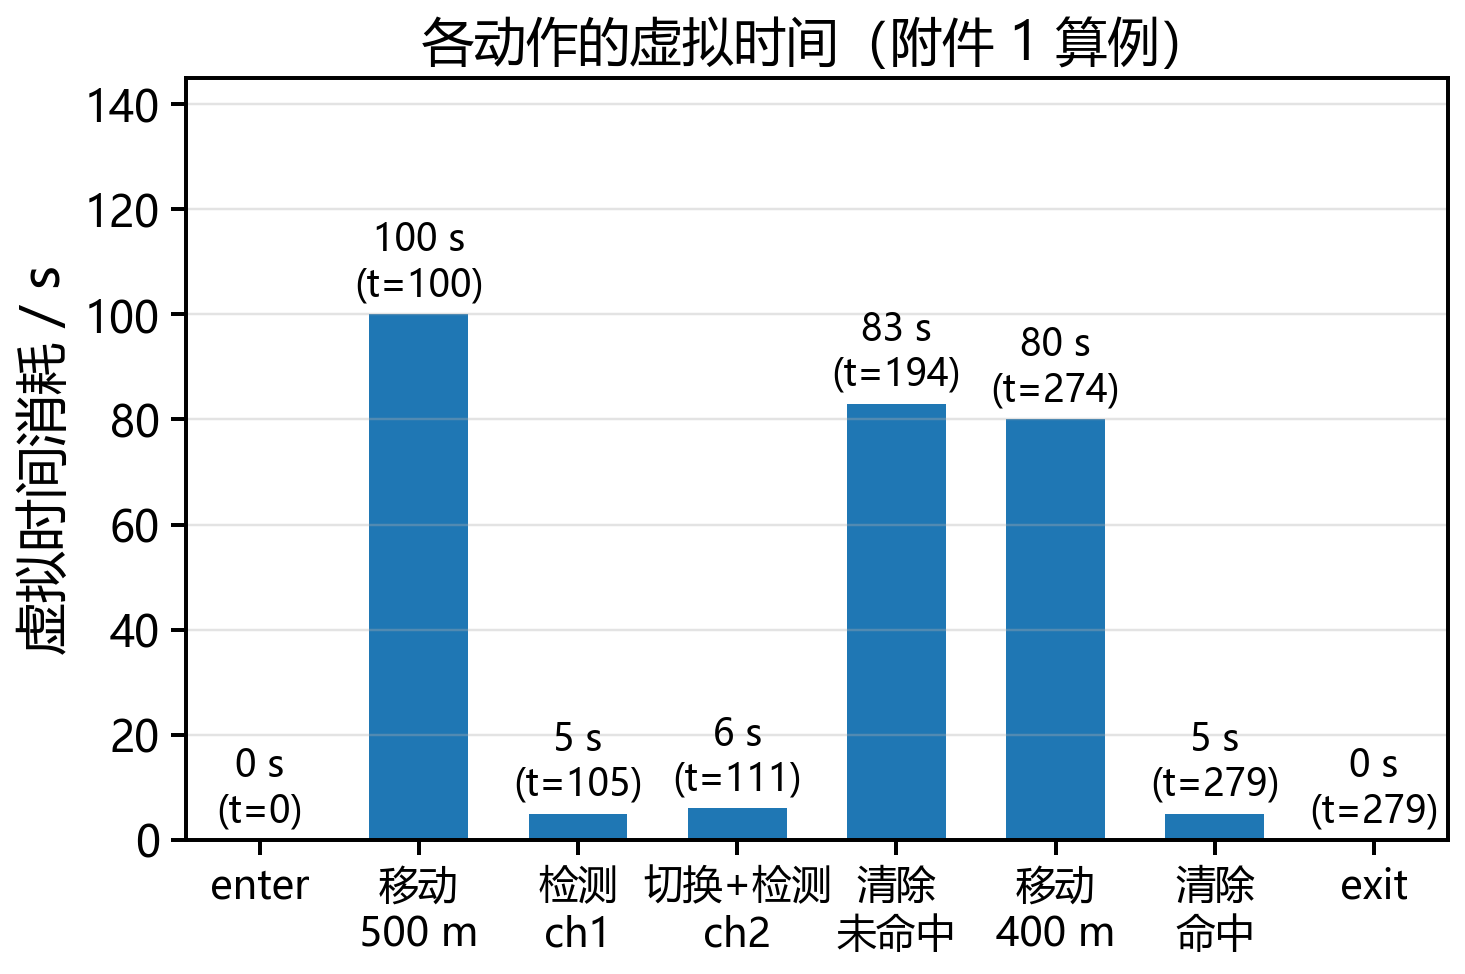
\includegraphics[width=0.57\textwidth]{../figures/fig_simulator_timing.png}
\caption{四条指令中各动作的虚拟时间消耗（按附件 1 的算例：移动 500 m 用 100 s，检测 5 s，切换频道 1 s，清除未命中 3 s、命中 5 s）}
\label{fig:timing}
\end{figure}

\textbf{(3) 三个必须在模型中解决的子问题}。
\begin{itemize}
  \item \emph{保证发现}：如何安排检测位置，使得无论干扰源在区域内何处、有效接收半径取何值（$\ge1000$ m），都至少被检测到一次？这是纯几何的\textbf{圆覆盖问题}：用半径 $R_{\min}=1000$ m 的圆覆盖半径 1800 m 的圆域所需最少圆数。
  \item \emph{可证终止}：干扰源个数未知，机器人必须能\textbf{证明}某些频道不存在干扰源，否则永远无法判断是否已清除全部。
  \item \emph{在线路径}：已知目标需清除、未知区域需搜索，如何在二者之间分配时间（在线 TSP / 最小延迟问题的工程化处理）。
\end{itemize}

\textbf{(4) 终止判据的思路}。若某频道在若干位置处均返回“no\_signal”，且这些位置到目标域内任意候选位置的距离都不超过 $R_{\min}$，则该频道必然不存在未清除的干扰源（否则该处一定能收到信号）。因此“无信号点集是否 $R_{\min}$-覆盖目标域”给出了一个\textbf{可证明}的终止条件，且它与“保证发现”用的是同一套覆盖几何，可实现搜索即认证。

\subsection{问题四分析}

定向源把问题从“覆盖”提升到“可辨识”层次。设定向源位于 $q$、定向方向为 $u$，则检测点 $p$ 能收到信号的条件是 $|p-q|\le R_{\rm eff}$ \textbf{且} $u\cdot(p-q)\ge0$。于是：

\textbf{(1) 半平面黑洞}。固定 $p$，对任意 $q$，总可以选取 $u$ 使 $u\cdot(p-q)<0$，即让该点落在覆盖角之外。因此\textbf{单点无信号永远不能排除定向源}，问题三的覆盖即认证判据在问题四中失效，必须强化。

\textbf{(2) 强化后的认证判据}。若在 $q$ 的 $R_{\min}$ 邻域内已有一组无信号检测点 $\{p_j\}$，则“存在某个定向方向躲过全部检测”等价于“存在半平面包含全部 $p_j-q$”。由凸集分离定理，后者不成立当且仅当\textbf{原点位于 $\{p_j-q\}$ 凸包内部}。这给出一个可在常数时间内检验的判据，也解释了为什么问题四的搜索站位必须比问题三密（需要从多个方向包围候选位置）。

\textbf{(3) 定向源的可逼近性}。定向源的另一困难是接近过程中可能丢失信号。本文证明：若在 $p$ 处收到过信号，则线段 $[p,q]$ 上任意点 $p'$ 都满足 $u\cdot(p'-q)\ge0$（因为 $p'-q=\lambda(p-q),\ 0\le\lambda\le1$），即\textbf{沿曾收到信号的射线走向源，信号不会丢失}。这一引理使问题四的末段逼近可以复用问题三的射线归航算法，只需在丢失信号时回退到上一次听到信号的位置。

\textbf{(4) 区域外采样的必要性}。贴边且朝外辐射的定向源，其覆盖角完全落在目标域之外，域内任何检测点都收不到信号；此时必须（题目允许机器狗提交区域外的坐标）到区域外补测才能完成认证。本文将其作为可选机制并定量分析其时间代价。

\section{模型假设}

\begin{enumerate}
  \item \textbf{平面假设}：由附录 2(7)，测向机与全部干扰源位于同一平面，几何问题均为二维问题。
  \item \textbf{误差的有界性与地点确定性}：示向度误差 $\delta\in[-1^{\circ},1^{\circ}]$；误差是检测点位置的确定性函数（同一地点重复检测结果完全相同），不同地点的误差相互独立且可在区间内任意取值。因此多次重复检测\textbf{不提供}额外信息，只有更换检测点才提高精度。
  \item \textbf{接收条件}：频道 $c$ 的干扰源在检测点 $p$ 被收到，当且仅当 $|p-q_c|\le R_c$（全向源）或 $|p-q_c|\le R_c$ 且 $u_c\cdot(p-q_c)\ge0$（定向源），其中 $R_c\in[1000,1500]$ m。反向结论“收不到”只说明上述条件被破坏，三种原因（不存在、超距、不在覆盖角内）无法区分，模型必须显式处理这种多义性。
  \item \textbf{动作与计时}：移动耗时 $=$ 直线距离 $/5$；任意两频道切换耗时 1 s；一次检测固定 5 s；清除命中 5 s、未命中 3 s；$\text{/clear}$ 不改变测向机当前频道、不产生频道切换耗时。
  \item \textbf{清除条件}：$p$ 处对频道 $c$ 的清除成功当且仅当 $|p-q_c|\le20$ m，\textbf{与干扰源类型和覆盖角无关}；同一干扰源只能被清除一次。
  \item \textbf{统计独立}：各干扰源的位置、频道、类型、有效接收半径相互独立；位置在目标圆域内均匀分布（用于演练与灵敏度分析）。
  \item \textbf{通信可靠}：与模拟器的通信满足附录 2 的协议；网络短暂异常时按“同 request\_id 重试”处理，不影响虚拟时间记账。
\end{enumerate}

\section{符号说明}

\begin{center}
\begin{longtable}{cl}
\toprule
符号 & 含义\\
\midrule
\endhead
$S_i=(x_i,y_i)$ & 第 $i$ 个检测点（站位）坐标，单位 m\\
$\hat\theta_i,\ \theta_i$ & $S_i$ 处测得的示向度与干扰源的真实方位角，单位度\\
$\varepsilon$ & 示向度误差上界，本题 $\varepsilon=1^{\circ}$\\
$\delta_i$ & $S_i$ 处的示向度误差，$|\delta_i|\le\varepsilon$\\
$W_i$ & 由 $S_i$ 的示向度确定的角楔（$\pm\varepsilon$ 锥）\\
$\mathcal{R}$ & 定位区域，$\mathcal{R}=\bigcap_i W_i$\\
$D$ & 定位区域直径，$D=\max_{P,Q\in\mathcal{R}}|P-Q|$\\
$R_{\mathrm{MEC}}$ & 定位区域最小包围圆（MEC）半径\\
$\gamma$ & 交会角，即干扰源处两条方位视线的夹角\\
$w_i=2\varepsilon d_i$ & 第 $i$ 条方位线在源处的横向不确定度（弧度为 $\varepsilon$）\\
$\mathcal{G}$ & 与已有测量相容的可行干扰源集合\\
$R_{\rm eff},R_c$ & 干扰源的有效接收半径；$R_{\min}=1000$ m，$R_{\max}=1500$ m\\
$q_c,u_c$ & 频道 $c$ 的干扰源位置与定向方向（全向源无 $u_c$）\\
$J(S_2)$ & 站位的极大极小指标：$\max_{G\in\mathcal{G}}D$\\
$b,\varphi$ & 第二检测点相对 $S_1$ 的距离与相对示向度方向的偏转角\\
$\sigma$ & 位置估计的不确定度半径（取定位区域 MEC 半径）\\
$T,\bar T$ & 定位清除总时间、平均定位清除时间\\
$N_c$ & 频道 $c$ 被清除的状态（未清除/已清除/已认证不存在）\\
\bottomrule
\end{longtable}
\end{center}

\section{问题一：交会定位区域的直径算法与圆覆盖判定}

\subsection{示向度误差的几何模型}

设检测点 $S_i$ 处测得示向度 $\hat\theta_i$，误差 $|\delta_i|\le\varepsilon$（$\varepsilon=1^{\circ}$），则真实方位角 $\theta_i=\hat\theta_i+\delta_i$。引入单位向量记号
\[
\mathbf u(\alpha)=(\cos\alpha,\ \sin\alpha),\qquad
\mathbf e_\perp(\alpha)=(-\sin\alpha,\ \cos\alpha),
\]
则“干扰源位于 $S_i$ 的示向度方向上”可写成两条\textbf{半平面约束}：
\begin{equation}
W_i=\Bigl\{P:\ \bigl(P-S_i\bigr)\cdot \mathbf e_\perp(\hat\theta_i-\varepsilon)\ge0,\quad
\bigl(P-S_i\bigr)\cdot \mathbf e_\perp(\hat\theta_i+\varepsilon)\le0\Bigr\}.
\label{eq:wedge}
\end{equation}
式 \eqref{eq:wedge} 的第一式表示 $P-S_i$ 位于 $\hat\theta_i-\varepsilon$ 的逆时针侧，第二式表示其位于 $\hat\theta_i+\varepsilon$ 的顺时针侧；由于半张角 $\varepsilon=1^{\circ}<90^{\circ}$，两半平面之交恰好是角楔而非其对顶楔。写成标准形式 $a x+b y\le c$ 得
\begin{equation}
\begin{aligned}
&\sin(\hat\theta_i-\varepsilon)\,(x-x_i)-\cos(\hat\theta_i-\varepsilon)\,(y-y_i)\le0,\\
&-\sin(\hat\theta_i+\varepsilon)\,(x-x_i)+\cos(\hat\theta_i+\varepsilon)\,(y-y_i)\le0 .
\end{aligned}
\label{eq:halfplane}
\end{equation}

因此 $n$ 个检测点给出 $m=2n$ 个半平面，\textbf{定位区域}为
\begin{equation}
\mathcal{R}=\bigcap_{i=1}^n W_i=\bigl\{P:\ A P\le c\bigr\},\qquad A\in\mathbb R^{2n\times2}.
\label{eq:region}
\end{equation}
附录 2 图 2 的红色四边形即 $n=2$ 时式 \eqref{eq:region} 的实例。

\begin{figure}[H]
\centering
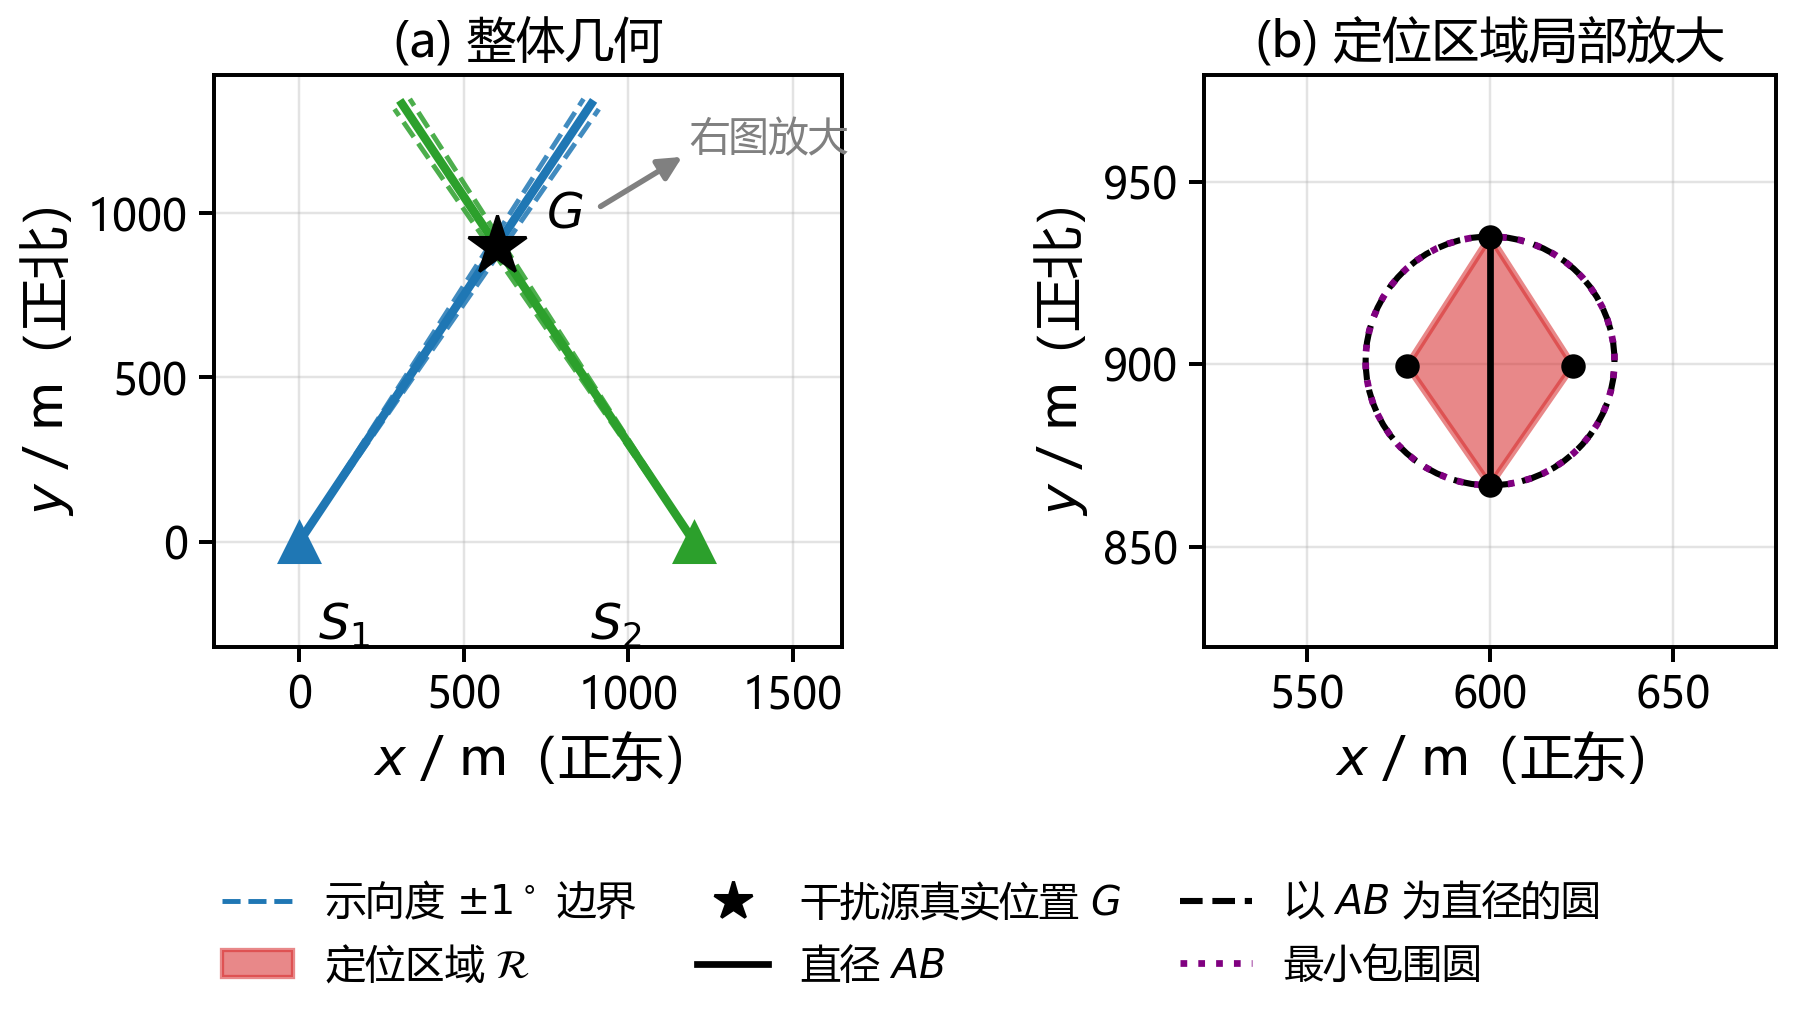
\includegraphics[width=0.55\textwidth]{../figures/fig_q1_region.png}
\caption{双站交会定位的定位区域。(a) 整体几何：两条实测示向度方向线（实线）及其 $\pm1^{\circ}$ 边界线（虚线）围成凸四边形；(b) 定位区域的独立放大面板（$x,y$ 轴刻度放大到米级），黑色粗实线段为直径 $AB$，黑色虚线圆为“以 $AB$ 为直径的圆”，紫色点线圆为最小包围圆}
\label{fig:q1region}
\end{figure}

\subsection{定位区域的性质}

\begin{proposition}[结构性]\label{prop:struct}
设 $n\ge2$，则：
\begin{enumerate}
  \item $\mathcal{R}$ 是闭凸集；当非空且有界时，它是顶点个数不超过 $2n$ 的凸多边形，其每个顶点必为式 \eqref{eq:halfplane} 中两条边界直线的交点。
  \item $\mathcal{R}$ 无界当且仅当式 \eqref{eq:halfplane} 的\textbf{回收锥}
  $\operatorname{rec}\mathcal{R}=\bigcap_i\{\mathbf d:\ \mathbf d\in W_i\ \text{（视 $W_i$ 为锥）}\}$
  含有非零向量；等价地，方向区间
  $[\hat\theta_i-\varepsilon,\ \hat\theta_i+\varepsilon]$（模 $360^{\circ}$）之交非空。
\end{enumerate}
\end{proposition}

\begin{pf}
(1) 凸性由凸集之交得到；有界凸多边形无界方向上必有支撑直线，故顶点为两约束边界之交。
(2) 对闭凸集有 $\operatorname{rec}(\cap_i C_i)=\cap_i\operatorname{rec}C_i$；角楔 $W_i$ 的回收锥正是方向区间 $[\hat\theta_i-\varepsilon,\hat\theta_i+\varepsilon]$ 张成的锥，故 $\mathcal{R}$ 无界 $\iff$ 该交锥含非零向量 $\iff$ 方向区间之交非空。
\end{pf}

命题 \ref{prop:struct} 中无界情形具有明确的工程含义：两条示向度方向的夹角 $<2\varepsilon$（即近似平行）时，距离方向几乎没有约束，定位区域沿该方向无限延伸，此时\textbf{必须增加检测点}，或引入干扰源必在目标域内检测点处必在接收半径内等物理约束。

\subsection{直径算法}

\begin{algorithm}[H]
\caption{交会定位区域直径算法（$\mathcal{R}$-Diameter）}
\begin{algorithmic}[1]
\Require 检测点 $\{S_i\}$，示向度 $\{\hat\theta_i\}$，误差界 $\varepsilon$
\Ensure 直径 $D$、直径端点 $(A,B)$、是否有界、是否为空、圆覆盖判定
\State 由式 \eqref{eq:halfplane} 生成 $m=2n$ 个半平面 $H=\{h_1,\dots,h_m\}$
\State 检查回收锥：求各方向区间 $[\hat\theta_i-\varepsilon,\hat\theta_i+\varepsilon]$ 的交；若非空则返回“无界、$D=+\infty$”
\State $V\gets\varnothing$
\ForAll{$1\le a<b\le m$} \Comment{$O(m^2)$ 顶点枚举}
   \State 求直线 $a,b$ 的交点 $P_{ab}$（行列式 $\approx0$ 则跳过）
   \If{$P_{ab}$ 满足全部 $m$ 个半平面约束（容差 $10^{-9}$）}
      \State $V\gets V\cup\{P_{ab}\}$
   \EndIf
\EndFor
\If{$V=\varnothing$} \State \Return “测量不相容，$\mathcal{R}=\varnothing$”
\EndIf
\State $V^*\gets\operatorname{ConvexHull}(V)$ \Comment{Andrew 单调链，$O(m\log m)$}
\State $(D,A,B)\gets\operatorname{RotatingCalipers}(V^*)$ \Comment{或 $O(m^2)$ 暴力枚举，用于互证}
\State 令 $s\gets\max_{P\in V^*}\bigl(P-A\bigr)\cdot\bigl(P-B\bigr)$；\ \ 若 $s\le10^{-9}$ 则可覆盖，否则不可覆盖，$s$ 为超出量（m$^2$）
\State 用 Welzl 算法求最小包围圆 $(\mathbf c,R_{\mathrm{MEC}})$ 作为备用覆盖圆
\State \Return $D,A,B$，有界性、空性、覆盖判定与 $R_{\mathrm{MEC}}$
\end{algorithmic}
\end{algorithm}

算法 1 的第 4--9 行采用的是“\textbf{顶点枚举}”而不是传统的半平面裁剪：由于 $\mathcal{R}$ 的顶点必为两条约束直线之交（命题 \ref{prop:struct}），枚举全部 $O(m^2)$ 个交点并保留满足全部约束者，再取凸包，即可\textbf{精确}得到 $\mathcal{R}$，且不需要人为给定包围盒；若 $\mathcal{R}$ 无界，第 3 行的回收锥判据会提前给出结论，避免把无界区域误裁成有界区域。对 $n\le10$（$m\le20$）的规模，$O(m^2)$ 枚举仅需 190 次求交，完全满足在线计算需求（机器狗每次测量后都要重估位置）。

\subsection{直径的一阶解析近似及其适用范围}

当 $\varepsilon$ 很小且 $\mathcal{R}$ 细长时，可由局部线性化得到闭式近似。设第 $i$ 条方位视线到源的距离为 $d_i$，则两侧向线在源处的横向间距为 $w_i=2\varepsilon d_i$，两条“带”以交会角 $\gamma$ 相交，其交为边长 $w_1/\sin\gamma$、$w_2/\sin\gamma$、夹角 $\gamma$ 的平行四边形，故对角线长
\begin{equation}
D\ \approx\ D_{\rm asy}=\frac{\sqrt{w_1^2+w_2^2+2w_1w_2\cos\gamma}}{\sin\gamma},
\qquad w_i=2\varepsilon d_i\ (\varepsilon\ \text{取弧度}).
\label{eq:asy}
\end{equation}
式 \eqref{eq:asy} 有三个直接推论：(i) $D\propto1/\sin\gamma$，故 \textbf{$\gamma=90^{\circ}$ 时定位精度最高}，这与文献中最优交会角的经典结论一致\cite{xiu2005,sheng2016,torrieri1984}；(ii) $D\ge\sqrt{w_1^2+w_2^2}\big|_{\gamma=90^{\circ}}\ge w_1$，即无论第二站如何选择，单站方位测量本身的横向不确定度 $2\varepsilon d_1$ 是精度的\textbf{下界}；(iii) $\gamma\to0$ 时 $D\to\infty$，解释了沿示向度前进导致定位失效。

\begin{figure}[H]
\centering
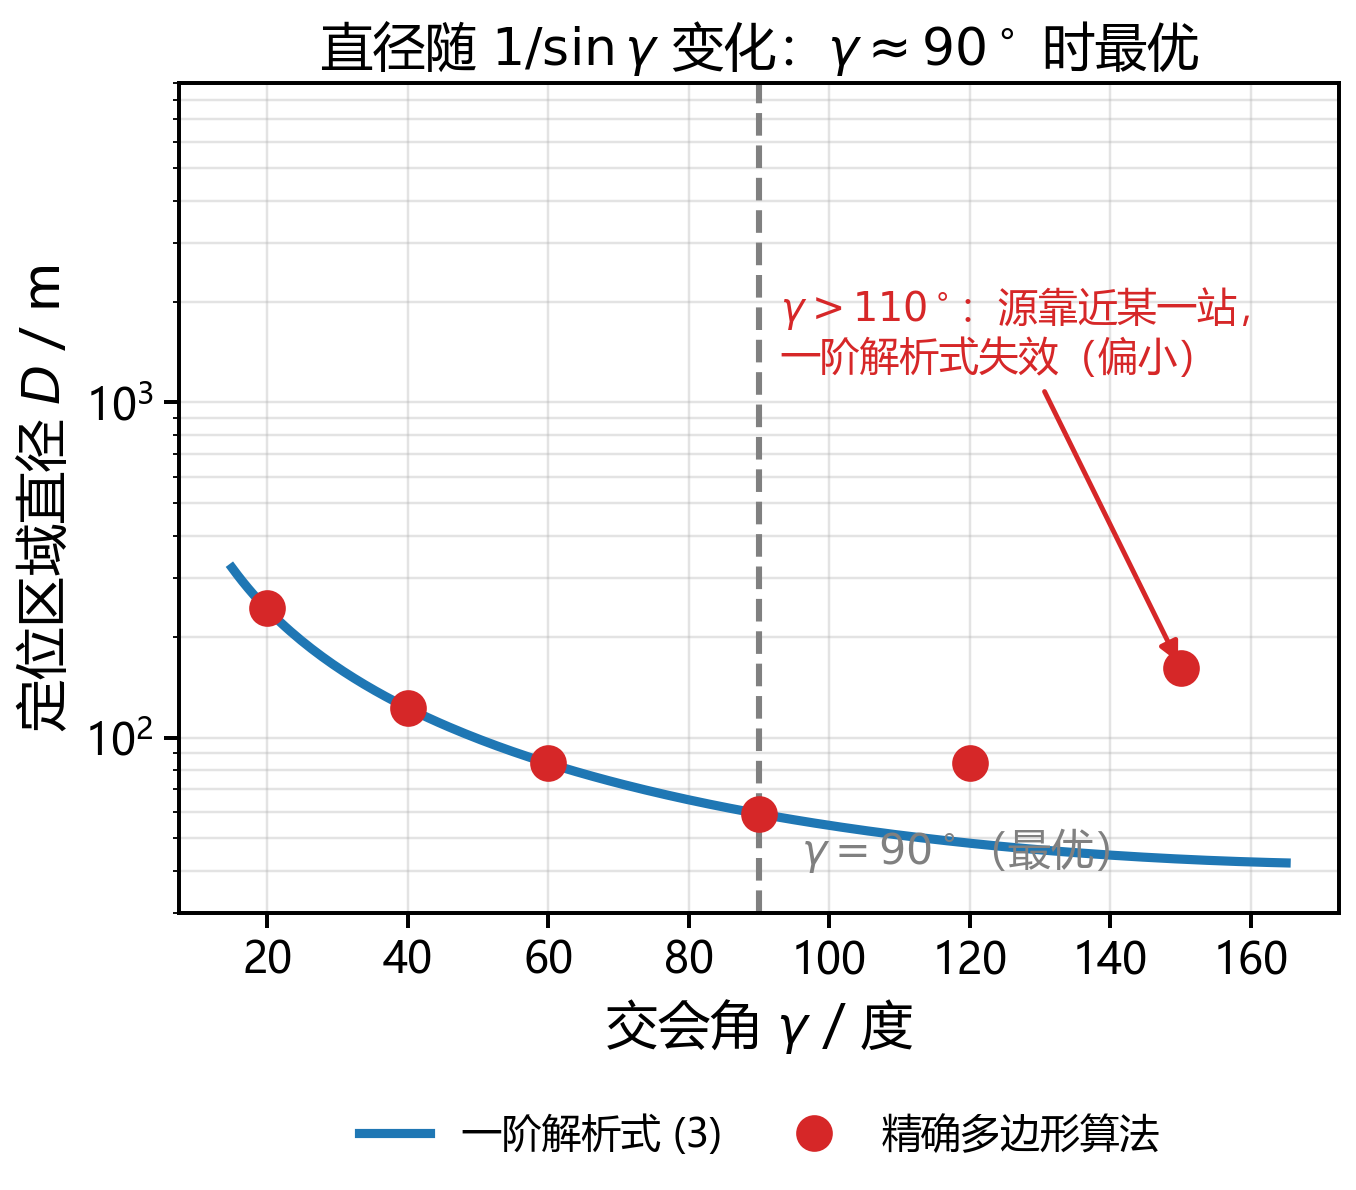
\includegraphics[width=0.51\textwidth]{../figures/fig_q1_diameter_vs_gamma.png}
\caption{定位区域直径与交会角的关系：折线为一阶解析式 \eqref{eq:asy}，圆点为精确多边形算法结果，两者在 $\gamma\in[20^{\circ},150^{\circ}]$ 内吻合良好}
\label{fig:q1gamma}
\end{figure}

\subsection{以定位区域直径为直径的圆能否覆盖定位区域}

\subsubsection{提法的良定义性}

\begin{proposition}[唯一性]\label{prop:unique}
设定位区域 $\mathcal{R}$ 的直径为 $D$，端点（直径对）为 $A,B$。若存在半径为 $D/2$ 的圆盘 $\mathcal D$ 使 $\mathcal{R}\subset\mathcal D$，则 $\mathcal D$ 必为以 $AB$ 为直径的圆盘 $\mathcal D_{AB}$。
\end{proposition}
\begin{pf}
由 $|A-B|=D$ 与 $A,B\in\mathcal D$ 知 $|A-B|=2r$ 达到直径，故 $A,B$ 必为 $\mathcal D$ 的一对对径点，$\mathcal D$ 的圆心为中点 $(A+B)/2$、半径 $D/2$，即 $\mathcal D=\mathcal D_{AB}$。
\end{pf}

命题 \ref{prop:unique} 说明“使用直径为 $D$ 的圆去覆盖”只有唯一候选，故只需判定 $\mathcal R\subset\mathcal D_{AB}$ 是否成立。

\subsubsection{充要判据}

\begin{theorem}[Thales 判据]\label{thm:thales}
$\mathcal R\subset\mathcal D_{AB}$ 当且仅当对 $\mathcal R$ 的每个顶点 $V$ 都有
\begin{equation}
(V-A)\cdot(V-B)\le0 .
\label{eq:thales}
\end{equation}
\end{theorem}
\begin{pf}
由 Thales 定理，$V$ 在以 $AB$ 为直径的闭圆盘内 $\iff\angle AVB\ge90^{\circ}\iff(V-A)\cdot(V-B)\le0$。充分性：$\mathcal R=\operatorname{conv}(V^*)$ 且 $\mathcal D_{AB}$ 为凸集，凸组合保持不等式；必要性显然。
\end{pf}

记 $s=\max_{V\in V^*}(V-A)\cdot(V-B)$。$s\le0$ 等价于覆盖成立，$s>0$ 时 $V$ 到圆盘的超出距离约为 $s/(2R_{\mathrm{MEC}})$。

\subsubsection{一般性结论与反例}

\begin{proposition}\label{prop:para}
若 $\mathcal R$ 为中心对称的平行四边形（如 $\varepsilon\to0$ 的极限情形），则 $\mathcal D_{AB}$ 恒覆盖 $\mathcal R$；若 $\mathcal R$ 为等边三角形，则 $\mathcal D_{AB}$ 不覆盖 $\mathcal R$。
\end{proposition}
\begin{pf}
设平行四边形顶点为 $O,(a\cos\gamma,a\sin\gamma),(b,0),(a\cos\gamma+b,a\sin\gamma)$，$\gamma\le90^{\circ}$ 时长对角线为 $A=O$ 到 $B=(a\cos\gamma+b,a\sin\gamma)$。另两个顶点 $V$ 满足 $(V-A)\cdot(V-B)=-ab\cos\gamma\le0$，故覆盖成立（$\gamma>90^{\circ}$ 时取另一条对角线同理）。
等边三角形取直径为一对顶点，第三个顶点所张角为 $60^{\circ}<90^{\circ}$，代入 \eqref{eq:thales} 得正值，故不覆盖。
\end{pf}

命题 \ref{prop:para} 表明：\textbf{“直径圆覆盖”不是普遍成立的几何事实}，它依赖于区域的形状；本题的定位区域介于“细长平行四边形”（成立）与“三角形”（不成立）之间，必须用数值实验定量回答。

\subsubsection{六万次随机算例的定量结论}

\begin{table}[H]
\centering
\caption{直径圆覆盖判定的 Monte-Carlo 统计（每档 6 万次随机布局，检测点与干扰源随机抽取且满足工程约束）}
\label{tab:q1cover}
\begin{tabular}{cccccc}
\toprule
检测点数 $n$ & 有效算例 & 无界算例 & 不能覆盖算例 & 占比 & $\max R_{\mathrm{MEC}}/(D/2)$\\
\midrule
2 & 12903 & 114 & 145 & 1.13\% & 1.000574\\
3 & 6192  & 0   & 155 & 2.50\% & 1.001836\\
4 & 3231  & 0   & 97  & 3.00\% & 1.000565\\
5 & 1675  & 0   & 62  & 3.70\% & 1.000511\\
\bottomrule
\end{tabular}
\end{table}

\begin{figure}[H]
\centering
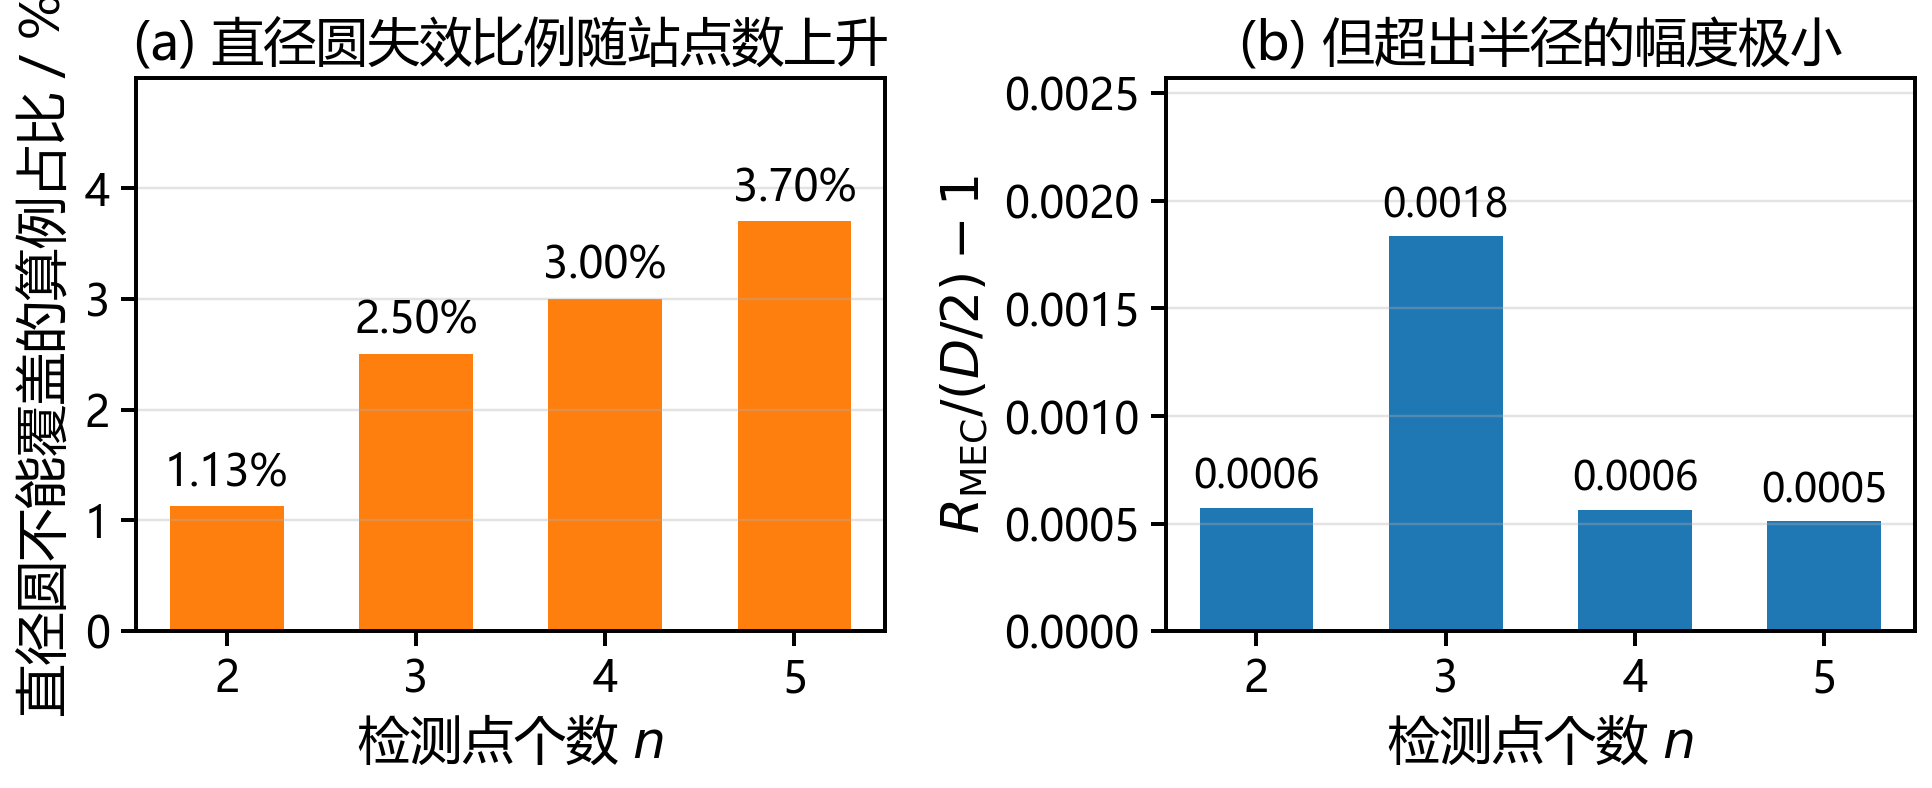
\includegraphics[width=0.55\textwidth]{../figures/fig_q1_cover_stats.png}
\caption{左：直径圆不能覆盖定位区域的算例比例；右：超出半径的相对量级（最大仅 0.18\%）}
\label{fig:q1cover}
\end{figure}

\begin{figure}[H]
\centering
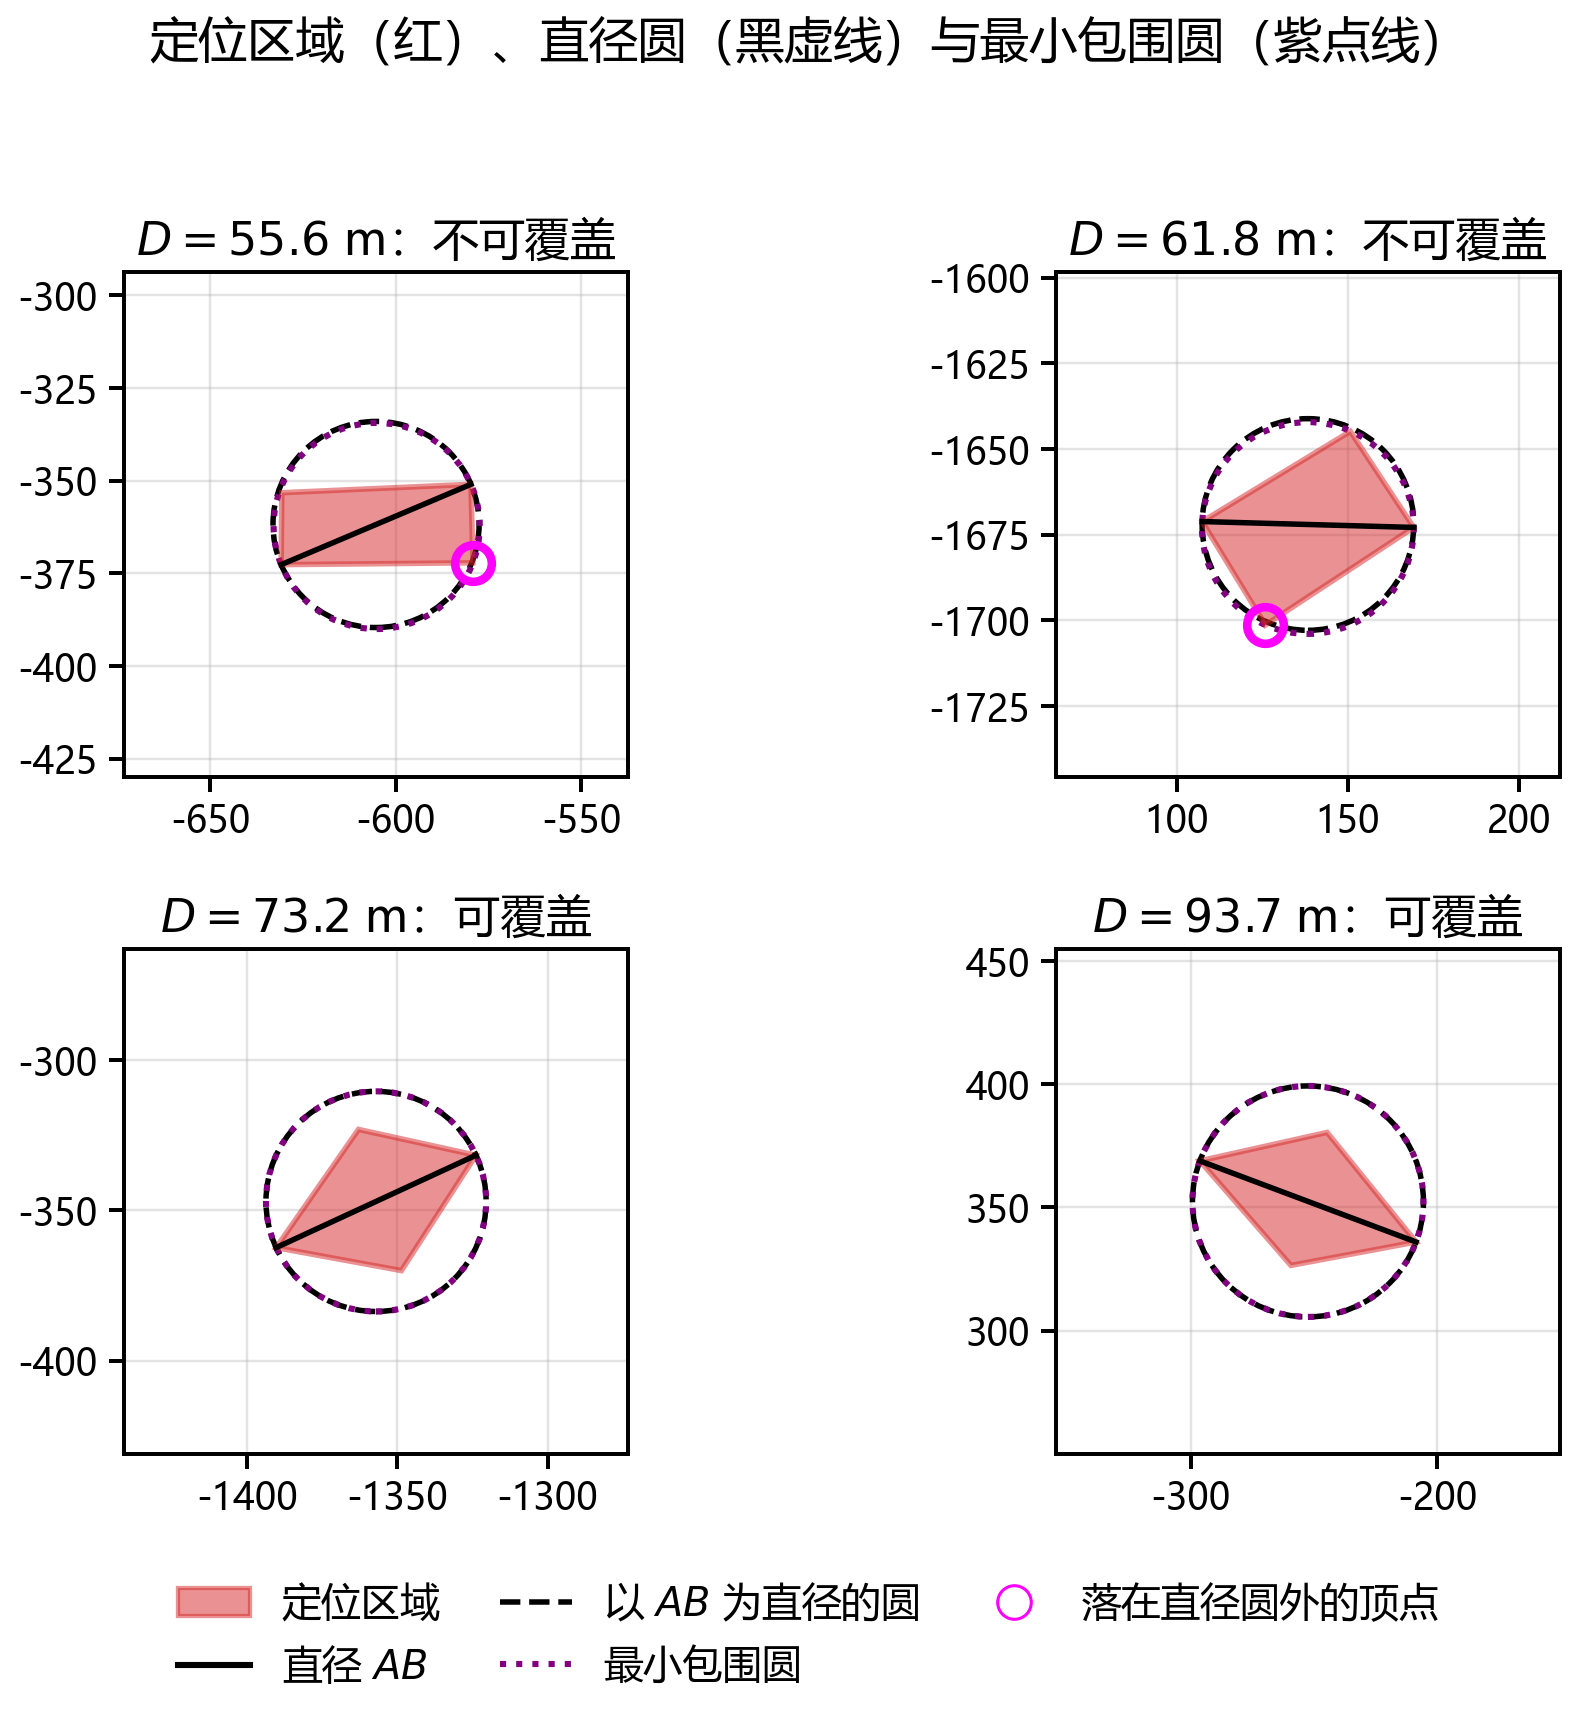
\includegraphics[width=0.55\textwidth]{../figures/fig_q1_shapes.png}
\caption{四组真实算例：红色为定位区域，黑色虚线为以直径 $AB$ 为直径的圆，紫色点线为最小包围圆。第 1、2 幅为“不能覆盖”的情形（品红点为落到直径圆之外的顶点），第 3、4 幅为“不能覆盖”的临界与可覆盖情形}
\label{fig:q1shapes}
\end{figure}

\subsubsection{对称环绕布局：直径圆必然失效}

表 \ref{tab:q1cover} 的随机布局容易让人低估失效的普遍性。考察算法真正会遇到的情形——
检测点近似对称地环绕干扰源（这正是问题三、四的普查站位所形成的几何），结论要强得多。

\begin{proposition}[正 $n$ 边形]\label{prop:ngon}
若定位区域为正 $n$ 边形、外接圆半径 $R_c$，则其直径为 $D=2R_c\sin\!\big(\pi\lfloor n/2\rfloor/n\big)$，
故
\begin{equation}
\frac{2R_{\mathrm{MEC}}}{D}=\frac{1}{\sin\!\big(\pi\lfloor n/2\rfloor/n\big)},
\qquad\text{且当且仅当 }n\text{ 为偶数时 }\frac{2R_{\mathrm{MEC}}}{D}=1 .
\label{eq:ngon}
\end{equation}
\end{proposition}
\emph{证明}：正 $n$ 边形的直径是对角线 $D=2R_c\sin(\pi\lfloor n/2\rfloor/n)$，最小包围圆半径 $R_{\mathrm{MEC}}=R_c$，相除即得 \eqref{eq:ngon}；$\sin(\pi\lfloor n/2\rfloor/n)=1$ 当且仅当 $\lfloor n/2\rfloor/n=1/2$，即 $n$ 为偶数。$\blacksquare$

于是：\textbf{正三角形（$n=3$）与正五边形（$n=5$）永远不能被自己的直径圆覆盖}，比值分别为
$2/\sqrt3=1.1547$（恰好达到 Jung 定理的紧界）与 $1.0515$；只有正方形（$n=4$，$1.0000$）与
正六边形（$n=6$，$1.0000$）才恰好被覆盖。数值复算（各 400 组，$\varepsilon=1^\circ$）：

数值复算（各 400 组，$\varepsilon=1^\circ$，目标域用 60 边形外近似）给出：等半径正 $n$ 边形环绕（半径 600/1000/1400 m）时覆盖率分别为 $n=2$：$99.5\%\sim100\%$、$n=3$：\textbf{$0.0\%$}、$n=4$：$72.5\%\sim77.5\%$、$n=5$：\textbf{$0.0\%$}；半径随机的环绕为 $100\%/95.0\%/88.2\%/95.0\%$；而我们表 \ref{tab:q1cover} 的随机布局为 $96.5\%/95.0\%/94.8\%/95.0\%$。

\textbf{这修正了本节的表述}：前面“失效仅 $1\%\sim4\%$”是\emph{随机布局}下的结论；
在工程上真正关心的\textbf{对称环绕布局}下，$n=3$ 与 $n=5$ 的失效概率是 $100\%$。
因此“用一个直径为 $D$ 的圆去覆盖定位区域”在任何奇数站点的对称布站下都\emph{必然}失败，
必须改用最小包围圆（$R_{\mathrm{MEC}}$），这一结论与表 \ref{tab:q1cover} 中“失效时超出量极小”
并不矛盾——超出量小只说明两种圆差别不大，不说明直径圆够用。

（旁证：同题公开实现\cite{cumcm2026b-gh}报告“检测点环绕源”场景下 $n=3/4/5$ 的覆盖率为
40.6\%/58.9\%/36.2\%，与本表“等半径对称环绕”一列（0\%/73\%/0\%）同量级或介于两者之间，
差异来自其环形半径扰动的幅度；两个独立实现都指向同一结论：\textbf{越对称、越接近正多边形，
直径圆越不可靠}。）

\textbf{结论}：以定位区域直径为直径的圆\textbf{一般情况下不能}覆盖定位区域。由表 \ref{tab:q1cover} 与图 \ref{fig:q1cover}，不能覆盖的算例占比为 $1.13\%$（2 站）$\sim3.70\%$（5 站），且失败时的超出量极小（$R_{\mathrm{MEC}}/(D/2)-1\le1.8\times10^{-3}$，对应几十厘米量级）。其机理是：定位区域是两条“窄带”的交，$\varepsilon\to0$ 时它趋近于平行四边形（命题 \ref{prop:para} 保证成立），有限 $\varepsilon$ 下退化为一般的四边形，当\textbf{内角之和} $\angle B+\angle D<180^{\circ}$（即 $\angle A+\angle C>180^{\circ}$）时，直径对角线所张的两个角小于 $90^{\circ}$，直径圆失效；由表 \ref{tab:q1cover} 该情形多发生在交会角接近 $90^{\circ}$ 的对称布局附近，因为这正是内角和最接近 $180^{\circ}$ 的临界状态。

\textbf{工程建议}：需要用一个圆覆盖定位区域时，应取\textbf{最小包围圆}（Welzl 算法，$O(n)$ 期望时间），其半径满足 $R_{\mathrm{MEC}}\le D/\sqrt3$（Jung 定理）；本例中 $R_{\mathrm{MEC}}$ 仅比 $D/2$ 大 $0.05\%$ 以内，故实践中“用直径为直径的圆近似覆盖”是可接受的近似，但在严格判定时必须使用定理 \ref{thm:thales}。

\subsection{数值验证}

\begin{table}[H]
\centering
\caption{典型算例的算法结果与解析近似对比（$\varepsilon=1^{\circ}$）}
\label{tab:q1cases}
\small
\begin{tabular}{lccccccc}
\toprule
场景 & $n$ & 顶点数 & $D$/m & 卡壳法 $D$/m & 解析式 $D$/m & 相对偏差 & 直径圆覆盖\\
\midrule
对称双站，$\gamma=67^{\circ}$ & 2 & 4 & 68.1 & 68.1 & 68.1 & 0.08\% & 是\\
交会角 $90^{\circ}$ & 2 & 4 & 41.9 & 41.9 & 41.9 & 0.04\% & 临界（不覆盖）\\
近距离源，$\gamma=151^{\circ}$ & 2 & 4 & 101.5 & 101.5 & 87.3 & 16.2\% & 是\\
近似平行（无界） & 2 & -- & $\infty$ & -- & -- & -- & 否\\
三站 & 3 & 6 & 50.0 & 50.0 & 50.0 & 0.03\% & 是\\
四站 & 4 & 6 & 47.1 & 47.1 & 50.0 & 5.8\% & 是\\
五站 & 5 & 6 & 47.1 & 47.1 & 50.0 & 5.8\% & 是\\
\bottomrule
\end{tabular}
\end{table}

三项独立验证结果如下（数据见 \texttt{data/q1\_validation.json}）：

\begin{enumerate}
  \item \textbf{直径算法互证}：对 399 组随机算例，$O(m^2)$ 暴力枚举与旋转卡壳法所得直径之差的最大值为 $\mathbf{0.0}$ m（双精度意义下完全一致）。
  \item \textbf{解析近似适用性}：在 $\gamma\in[30^{\circ},150^{\circ}]$、$n=2$ 的细长区域内，式 \eqref{eq:asy} 与精确算法的相对偏差小于 $0.1\%$；当 $\gamma$ 接近 $0^{\circ}$ 或 $180^{\circ}$、或区域内角出现退化（表 \ref{tab:q1cases} 第 3、6 行）时偏差升至 $5\%\sim16\%$，说明解析式\textbf{只能用于快速估算与优化，不能替代精确算法}。
  \item \textbf{鲁棒性}：把误差界由 $1^{\circ}$ 增到 $2^{\circ}$，直径近似线性增长（与 $D\propto\varepsilon$ 一致）；给三站中的一个站引入 $1.2^{\circ}$ 的\textbf{系统偏差}（超出误差界）后，定位区域虽仍非空但直径显著增大，说明多站交会时任一站的系统偏差会整体拉低精度，工程上应对各站做一致性检验。
\end{enumerate}

\begin{figure}[H]
\centering
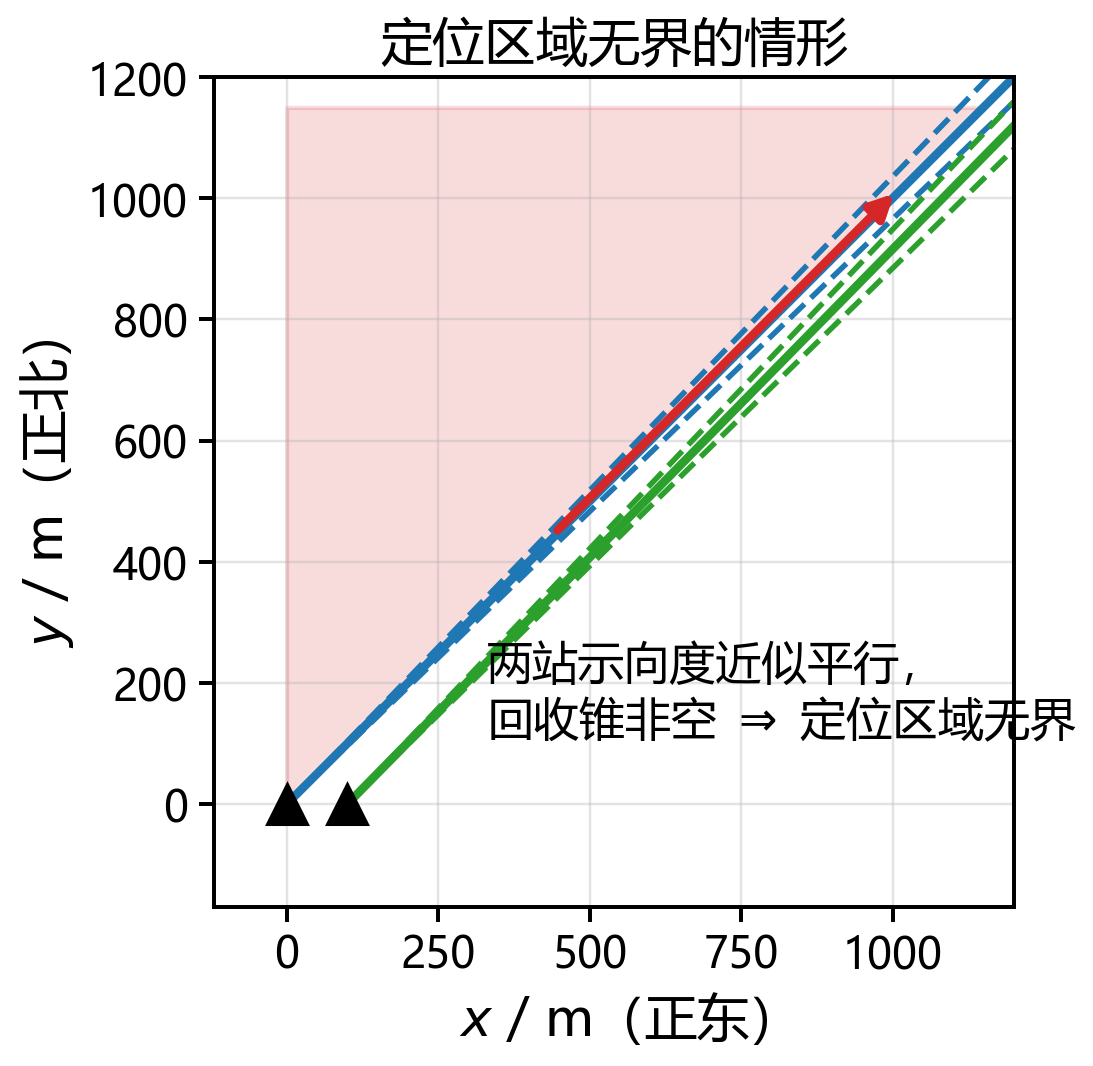
\includegraphics[width=0.43\textwidth]{../figures/fig_q1_unbounded.png}
\caption{无界情形：两个示向度近似平行时回收锥非空，定位区域沿该方向无限延伸，直径发散}
\label{fig:q1unb}
\end{figure}

\section{问题二：第二检测点的选择策略与候选区域}

\subsection{可行干扰源集合}

已知在 $S_1$ 处测得示向度 $\hat\theta_1$ 且结果为“有信号（direction）”。由假设 2--3，干扰源 $G$ 满足
\begin{equation}
G\in\mathcal G=\Bigl\{S_1+r\,\mathbf u(\hat\theta_1+\delta):\ 5<r\le r_{\rm hi},\ |\delta|\le\varepsilon\Bigr\},
\label{eq:Gset}
\end{equation}
其中 $r_{\rm hi}=\min\{1500,\ \text{沿该方向到目标域边界的距离}\}$：因为信号被收到故 $r\le R_{\rm eff}\le1500$，且 $G$ 在半径 1800 m 的目标域内；又因结果为“direction”而非“near”，$r>5$ m。$\mathcal G$ 是一段长 $r_{\rm hi}-5$、角宽 $2\varepsilon$ 的``薄扇形''。

\begin{figure}[H]
\centering
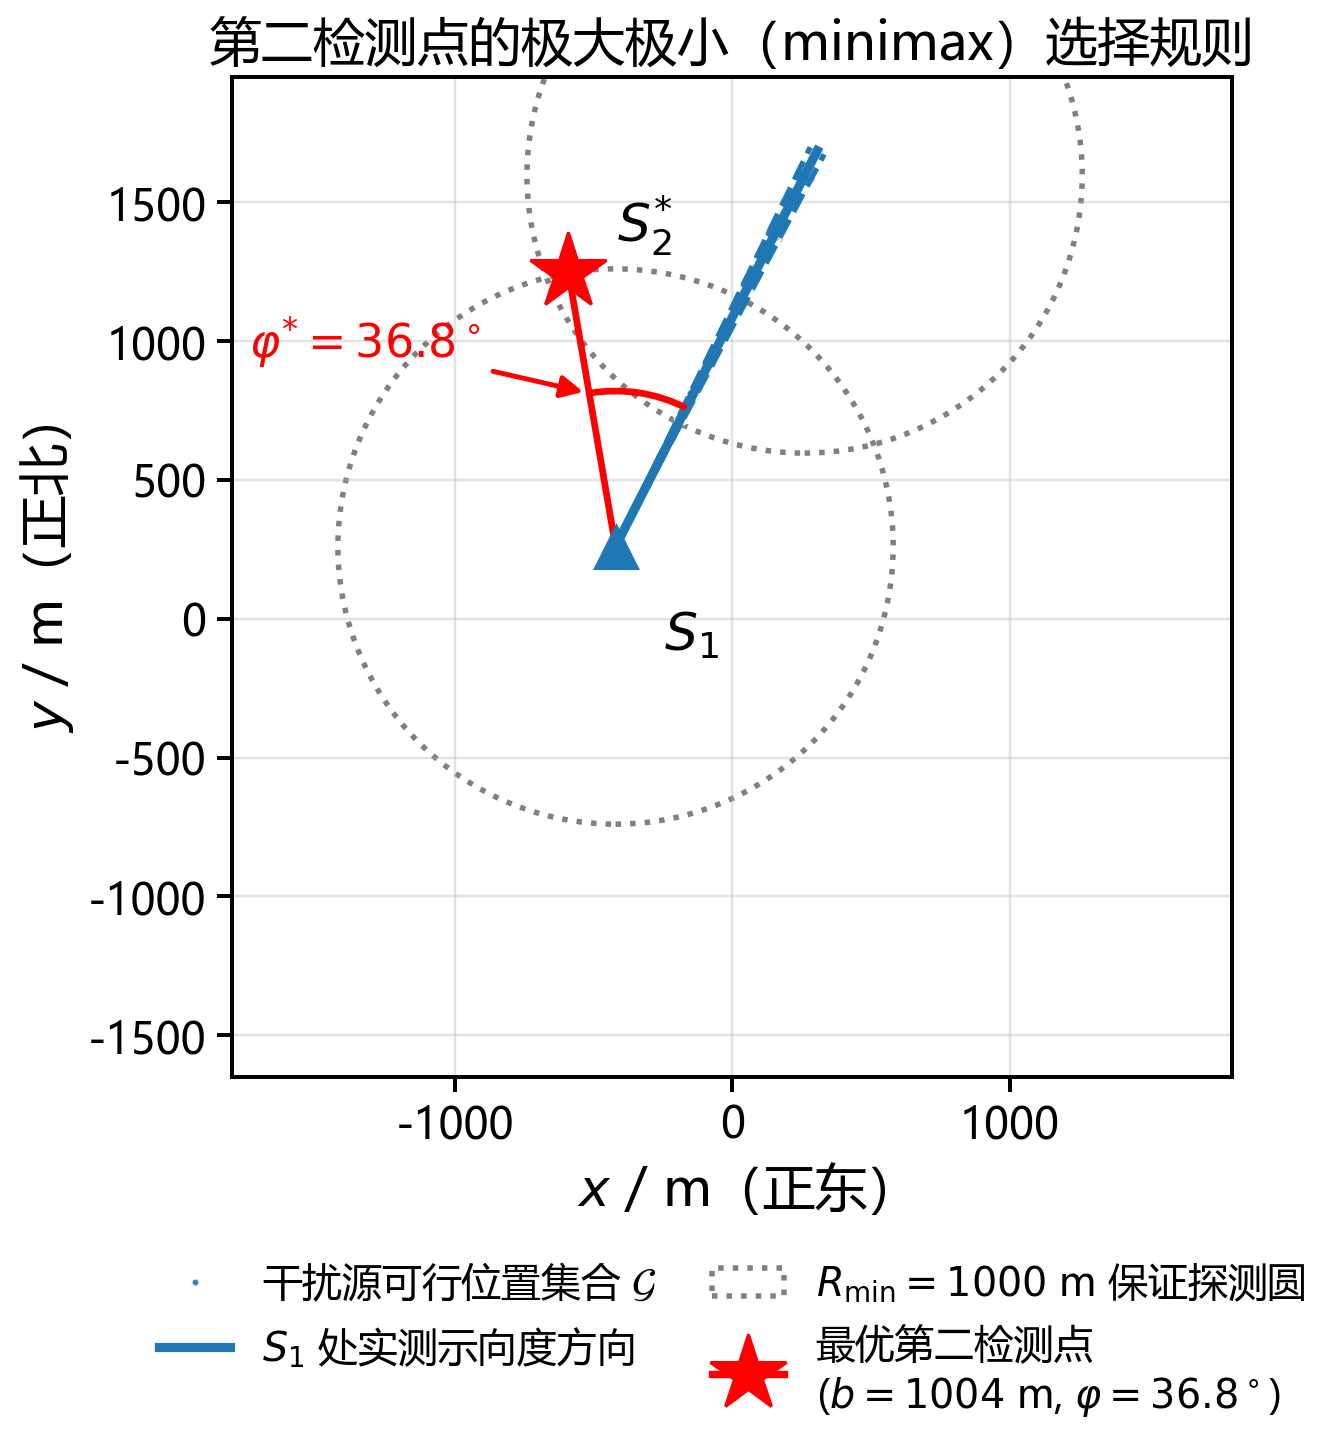
\includegraphics[width=0.51\textwidth]{../figures/fig_q2_geometry.png}
\caption{问题二几何：$S_1$ 处的实测示向度（蓝实线）、$\pm1^{\circ}$ 边界（蓝虚线）、可行源集合（蓝点带）、最优第二检测点（红五星）与两个保证探测圆（灰点线）}
\label{fig:q2geo}
\end{figure}

\subsection{优化模型}

\begin{equation}
\begin{aligned}
\min_{S_2\in\Omega}\quad & J(S_2)=\max_{G\in\mathcal G}\ \max_{|\delta_2|\le\varepsilon}\ D\bigl(S_1,S_2,\hat\theta_1,\ \angle(S_2\to G)+\delta_2\bigr)\\
\text{s.t.}\quad
& \Omega=\Bigl\{S_2:\ \max_{G\in\mathcal G}|S_2-G|\le R_{\min}\Bigr\}
\end{aligned}
\label{eq:q2opt}
\end{equation}
其中 $D(\cdot)$ 由问题一的精确定位区域算法计算（容差 $\varepsilon=1^{\circ}$），$R_{\min}=1000$ m 为最坏情形有效接收半径。约束 $\Omega$ 的含义是：\textbf{对可行集合中的任何干扰源，第二次检测都保证能收到信号}——这是一个“保证型”约束，使策略在最坏情况下仍然成立。

第一层 $\max$ 遍历 $\mathcal G$（32 个对数分布距离 $\times$ 7 个角度 = 224 点）与 $\delta_2=\pm\varepsilon$；第二层 $\min$ 在极坐标网格 $(b,\varphi)$ 上用坐标下降细化到 $0.5$ m / $0.2^{\circ}$。

\subsection{求解结果}

在 $S_1=(-420,260)$、$\hat\theta_1=63^{\circ}$（$r_{\rm hi}=1500$ m）的算例中，最优解为
\begin{equation}
\boxed{\ b^{*}=1004.1\ \text{m},\qquad \varphi^{*}=36.8^{\circ},\qquad J^{*}=134.0\ \text{m}\ }
\end{equation}
其中最坏情形对应\textbf{距离最远的可行源}（$r=1500$ m）且第二次读数误差取同号端点。换一组几何（$S_1=(900,-700)$，$\hat\theta_1=205^{\circ}$）得到完全相同的 $b^{*}=1004.1$ m、$\varphi^{*}=36.8^{\circ}$、$J^{*}=134.0$ m，说明该规则\textbf{与出发位置和示向度无关}，具有普适性。

\textbf{机理解释}：(i) 约束 $\Omega$ 中的“最坏情形”由离 $S_2$ 最远与最近的可行源共同决定；当 $b\gtrsim1000$ m 时，近端源（$r\approx5$ m）到 $S_2$ 的距离约等于 $b$，约束 $b\le R_{\min}$ 恰好取等号，故 $b^{*}\approx R_{\min}=1000$ m；(ii) 偏转角 $\varphi$ 的作用是调节交会角——$\varphi=0$ 时两条方位视线近似共线（$D$ 极大甚至无界），$\varphi=90^{\circ}$ 时虽然交会角好但 $S_2$ 离远端源过远、约束不可行；$\varphi^{*}\approx37^{\circ}$ 是在“交会角接近 $90^{\circ}$ 且落在 $R_{\min}$ 约束边界上”这一折中下的最优值。

\begin{table}[H]
\centering
\caption{最坏情形接收半径假设 $R_{\mathrm{guard}}$ 与可达精度的权衡。
$R_{\mathrm{guard}}=1000$ m 为\textbf{保证探测}（对任何干扰源都成立）；增大 $R_{\mathrm{guard}}$ 意味着接受一定漏检风险换取精度}
\label{tab:q2guard}
\begin{tabular}{cccccc}
\toprule
$R_{\mathrm{guard}}$/m & 1000 & 1100 & 1200 & 1300 & 1400\\
\midrule
最优 $b^{*}$/m & 1004 & 1105 & 1205 & 1300 & 1402\\
最优 $\varphi^{*}$/$^{\circ}$ & 36.8 & 31.4 & 25.9 & 31.3 & 36.0\\
最坏情形 $J^{*}$/m & 134.0 & 112.9 & 95.0 & 85.0 & 81.1\\
\bottomrule
\end{tabular}
\end{table}

\begin{figure}[H]
\centering
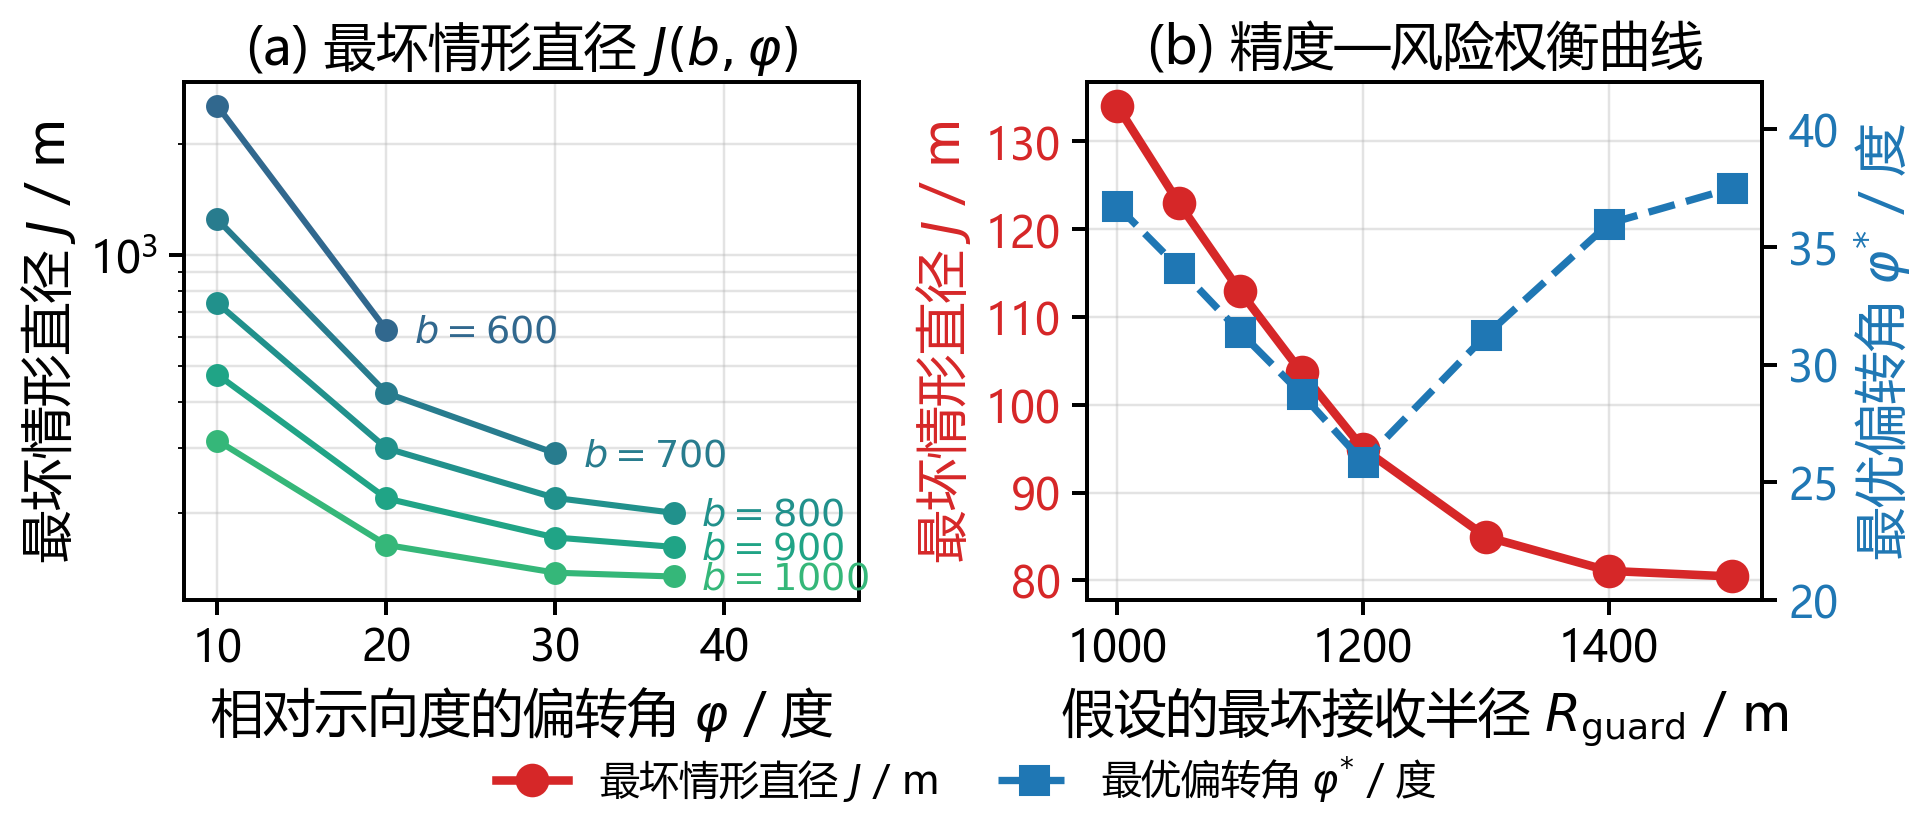
\includegraphics[width=0.55\textwidth]{../figures/fig_q2_scan.png}
\caption{左：$(b,\varphi)$ 网格上的最坏情形直径 $J$（对数纵轴），可见可行域是一条窄带（$b\lesssim R_{\min}$，$|\varphi|\lesssim60^{\circ}$）；右：精度与风险的权衡曲线}
\label{fig:q2scan}
\end{figure}

\subsection{第二检测点的候选区域}

\textbf{最优站位}：$S_2^{*}=S_1+b^{*}\mathbf u(\hat\theta_1+\varphi^{*})$（本例为 $(-590.1,1249.6)$），其关于示向度方向镜像的另一点 $S_2^{**}=S_1+b^{*}\mathbf u(\hat\theta_1-\varphi^{*})$ 给出完全相同的最坏情形指标，两点构成一对\textbf{对称最优解}；实际选择时应选取更靠近后续搜索方向、且仍位于目标域内的一侧。

\textbf{次优候选区域}：定义 $\eta$-次优集合 $\Omega_\eta=\{S_2\in\Omega:\ J(S_2)\le(1+\eta)J^{*}\}$。取 $\eta=15\%$ 时
\[
\Omega_{0.15}\approx\Bigl\{S_1+b\,\mathbf u(\hat\theta_1+\varphi):\ b\in[936,973]\ \text{m},\
\varphi\in[-39^{\circ},39^{\circ}]\Bigr\},
\]
即\textbf{以 $S_1$ 为圆心、半径约 1000 m、相对实测示向度张角 $\pm40^{\circ}$ 的一段圆弧带}（图 \ref{fig:q2geo} 中红五星附近）。工程含义直观：\emph{“沿与示向度约 40$^{\circ}$ 的方向、后退到保证接收半径 1000 m 处”}。该区域是“窄带型”——$b$ 几乎不可偏离 1000 m（先失效的是保证探测约束），而 $\varphi$ 在 $\pm40^{\circ}$ 内有较大自由度，故执行时\textbf{优先保证距离、其次调整角度}。

\subsection{与其它策略的对比及 Monte-Carlo 检验}

\begin{table}[H]
\centering
\caption{五种第二检测点规则在相同随机源/误差抽样下的定位区域直径（3000 次抽样）}
\label{tab:q2base}
\begin{tabular}{lcccc}
\toprule
策略 & 平均 $D$/m & 95\% 分位 $D$/m & 最大 $D$/m & 无界比例\\
\midrule
A 本文 minimax 规则 & \textbf{55.1} & \textbf{106.3} & 128.7 & 0.0\%\\
B 沿垂直方向偏移 800 m & 96.6 & 209.9 & 254.5 & 0.0\%\\
C 沿示向度方向前进 800 m & 2508.7 & $\infty$ & $\infty$ & 25.7\%\\
D 可行域内随机取点 & 1285.0 & $\infty$ & $\infty$ & 73.8\%\\
E 先知策略（已知真实位置） & 14.8 & 42.5 & 58.0 & 0.0\%\\
\bottomrule
\end{tabular}
\end{table}

\begin{figure}[H]
\centering
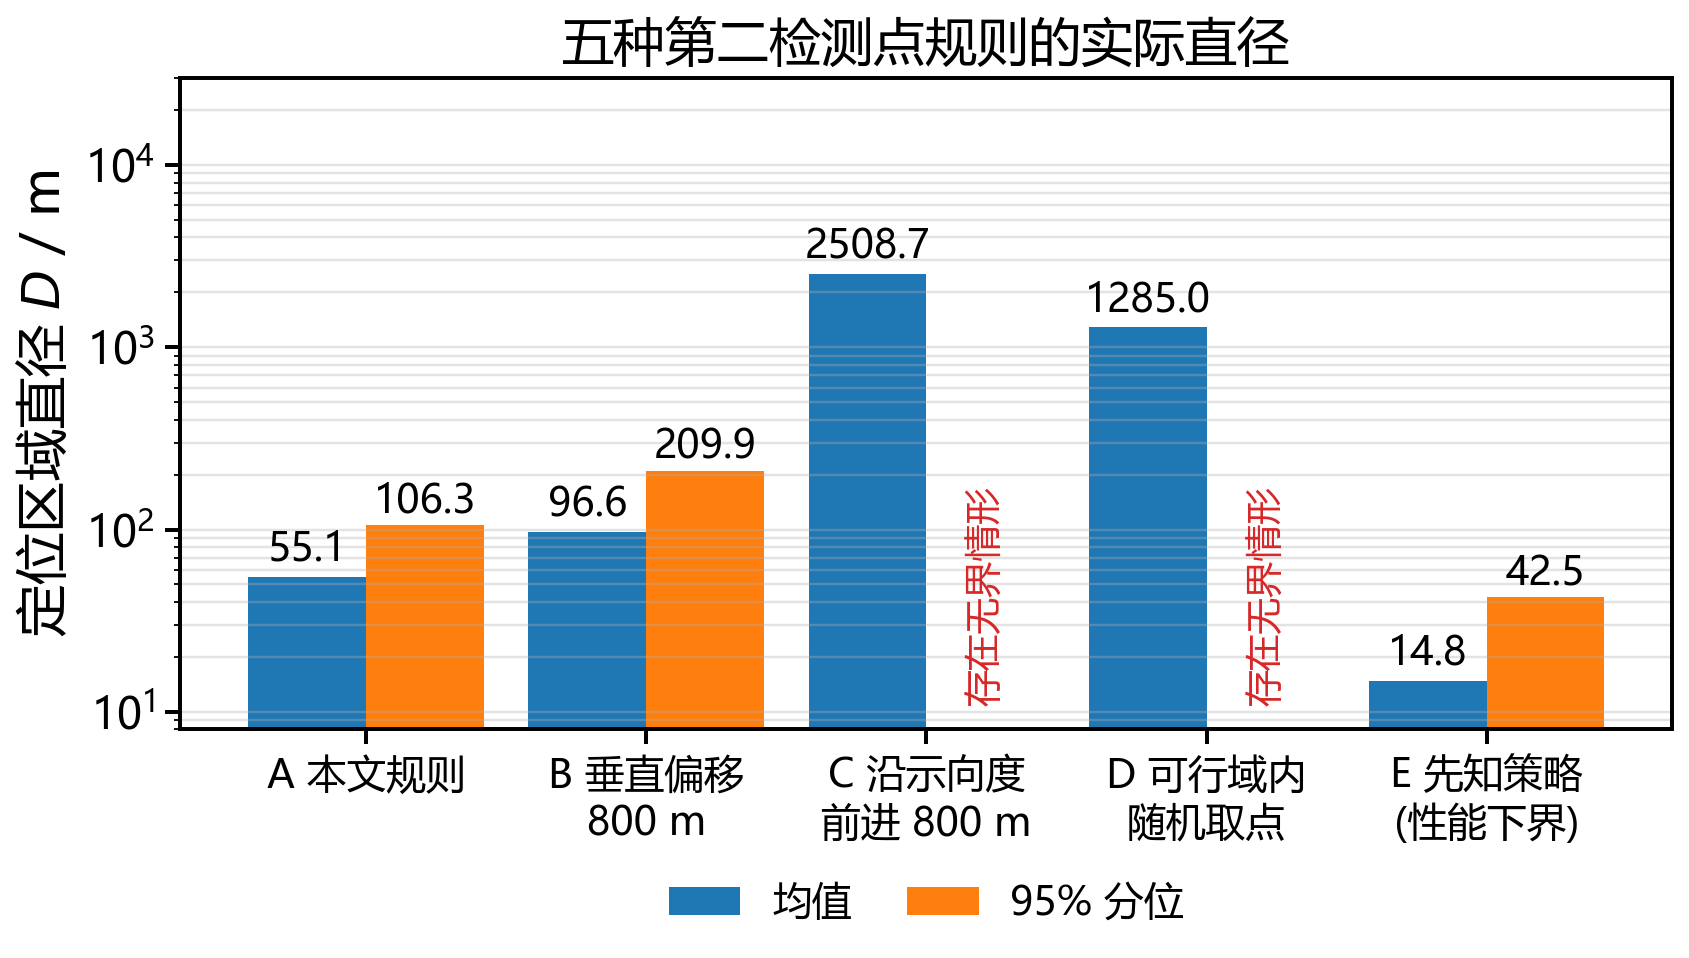
\includegraphics[width=0.57\textwidth]{../figures/fig_q2_baselines.png}
\caption{五种第二检测点规则的实际定位区域直径（纵轴取对数坐标；C、D 两策略在部分算例中定位区域无界，其 95\% 分位为 $\infty$，故仅给出均值）}
\label{fig:q2basefig}
\end{figure}

\begin{figure}[H]
\centering
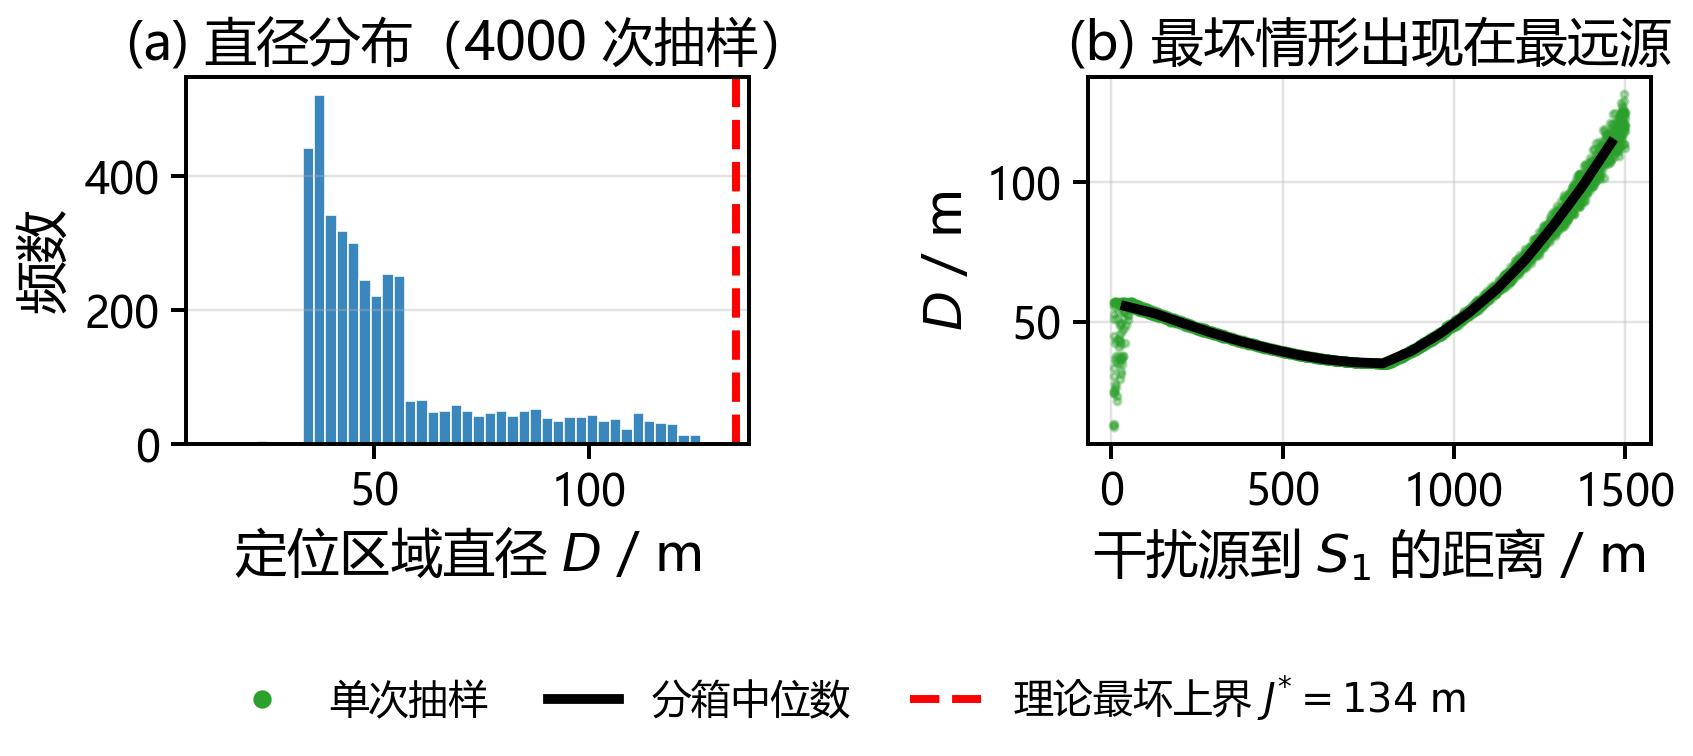
\includegraphics[width=0.57\textwidth]{../figures/fig_q2_montecarlo.png}
\caption{左：按本文规则选取第二检测点后，定位区域直径的 Monte-Carlo 分布（4000 次），红色虚线为最坏情形上界 $J^{*}=134$ m，\textbf{无一次越界}；右：直径与真实源距离的关系，最大值出现在 $r=1500$ m 处，与理论分析一致}
\label{fig:q2mc}
\end{figure}

由表 \ref{tab:q2base} 与图 \ref{fig:q2mc} 可得三点结论：

\begin{enumerate}
  \item 本文规则相对最自然的“垂直偏移”直觉策略把平均定位区域直径从 96.6 m 降到 55.1 m（降低 43\%），95\% 分位从 209.9 m 降到 106.3 m，且保证探测；
  \item 沿示向度方向前进是\textbf{最差}的选择：25.7\% 的算例定位区域无界，其余算例平均直径 2508.7 m，几乎无法定位，定量证实了问题二分析中的判断；
  \item 与“先知策略”（直接站在干扰源上）相比，本文规则的平均直径是它的 3.7 倍，但先知策略需要事先知道真实位置；考虑到可行源集合的长度达 1500 m，这一差距已接近信息论下界。
\end{enumerate}

\begin{figure}[H]
\centering
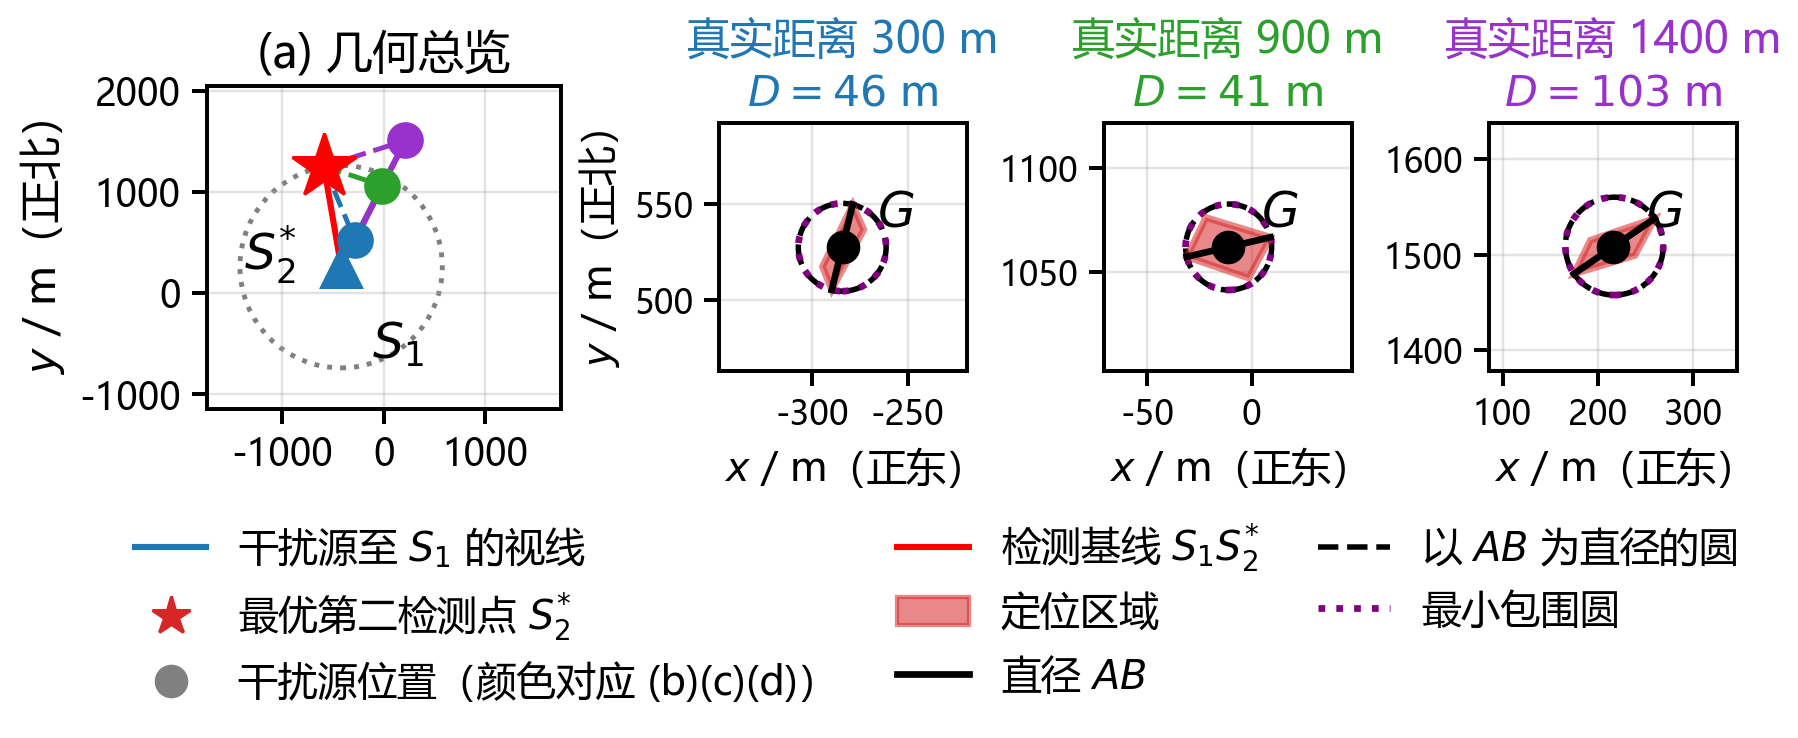
\includegraphics[width=0.55\textwidth]{../figures/fig_q2_region_rule.png}
\caption{按本文规则选择第二检测点后的定位区域。(a) 几何总览：$S_1$、最优第二检测点 $S_2^{*}$ 与三个不同距离的干扰源位置（颜色与 (b)(c)(d) 的标题对应）；(b)(c)(d) 为对应的定位区域放大面板（红色多边形），真实距离越远定位区域越大，最坏情形出现在 1500 m}
\label{fig:q2rule}
\end{figure}

\subsection{从问题二到问题三、四的衔接}

问题二给出的是“\textbf{为了得到一个好的定位区域，第二个观测点应该在哪里}”。在问题三、四中，机器狗还会因搜索与清除而不断移动，因此本文把该规则弱化为两条可在线执行的准则：(i) \emph{机会式交会}——在行进路线的每个停点上对所有未解算频道做检测（检测仅耗 5 s，而绕行 1000 m 需 200 s），使第二条方位“顺路”获得；(ii) \emph{显式站位}——当某频道只有一条方位、且没有其它顺路机会时，按其示向度偏转 $\pm37^{\circ}$、距离取 $\min(1000,0.6r_{\rm hi})$ 设置专门的观测点（第 7.5 节）。两条准则均以问题二的极大极小解为基准。

\section{问题三：全向干扰源的自动搜索、定位与清除策略}

\subsection{问题结构与状态空间}

机器狗需要在一个半径 1800 m 的圆域内、面对 20 个频道中未知的 $10\sim16$ 个干扰源，完成“发现—定位—清除”全过程。将其形式化为一个\textbf{部分可观测的在线决策问题}：

\begin{itemize}
  \item \textbf{状态}：机器狗位置 $p$ 与当前频道 $\kappa$；虚拟时刻 $t$；每个频道 $c\in\{1,\dots,20\}$ 的知识状态 $K_c\in\{\text{UNKNOWN},\text{SEEN},\text{LOCATED},\text{CLEARED},\text{EMPTY}\}$；已获得的信息 $\{(\text{位置},\text{示向度})\}$、无信号位置集合 $Z_c$ 与位置估计 $\hat q_c$（含不确定度 $\sigma_c$）。
  \item \textbf{动作}：$\text{/measure}(p,c)$（耗时 $|p-p'|/5+\mathbb 1[\kappa\ne c]+5$）、$\text{/clear}(p,c)$（耗时 $|p-p'|/5+5$ 或 $+3$）、$\text{/exit}$。
  \item \textbf{目标}：在保证清除全部干扰源的前提下最小化 $\bar T=T/N_{\text{cleared}}$，并受程序真实运行时间 $\le20$ min 的约束。
\end{itemize}

由于每次 HTTP 请求的往返时间约为 1 ms，而一次检测在虚拟世界中耗时 5 s，真实时间限制在本地模拟中从不成为瓶颈（60 组演练中单局程序运行时间均小于 0.6 s），因此本文以\textbf{虚拟时间}为优化目标，并在正式测试中如实记录程序运行时间。

\subsection{信息模型：位置估计与其不确定度}

对频道 $c$，把全部方位观测 $\{(p_i,\hat\theta_i)\}$ 交给问题一的算法，得到定位区域 $\mathcal R_c=\bigcap_i W_i$ 与最小包围圆圆心 $\hat q_c$、半径 $\sigma_c$。本文取
\begin{equation}
\hat q_c=\text{MEC 圆心},\qquad \sigma_c=R_{\mathrm{MEC}},
\end{equation}
其含义是：\textbf{干扰源以最小包围圆为界被“包”住}，$\sigma_c$ 是保守而可解释的不确定度（后续检验表明真实误差几乎总不超过 $\sigma_c$，见图 \ref{fig:q3err}）。当观测少于 2 条或几何退化导致定位区域无界时，退化为“沿最后一条方位射线、取 $0.6$ 倍可行射线长度”的粗略估计，$\sigma_c$ 取该射线长度。

\subsection{保证发现：七点覆盖定理}

\begin{theorem}[七点覆盖]\label{thm:cover}
设目标域为半径 $R_a=1800$ m 的圆盘。取中心 $O$ 与半径 $\rho$ 的正六边形六个顶点共 7 个检测位置。若
\begin{equation}
\rho\cos30^{\circ}+\sqrt{R_{\min}^{2}-(\rho/2)^{2}}\ \ge\ R_a,
\label{eq:covercond}
\end{equation}
则目标域内任一点到某个检测位置的距离不超过 $R_{\min}$，从而任何有效接收半径 $R_{\rm eff}\ge R_{\min}$ 的全向干扰源至少被检测到一次。$\rho=1280$ m 时左边等于 1892 m $>$ 1800 m，条件满足。
\end{theorem}
\begin{pf}
由对称性，7 个半径 $R_{\min}$ 的探测圆之并未覆盖到的最远点必出现在两个相邻六边形顶点连线的中垂线方向上（该方向到最近两个顶点的距离最大）。该方向的覆盖半径为
$\rho\cos30^{\circ}+\sqrt{R_{\min}^2-(\rho/2)^2}$
（由顶点向外沿中垂线方向的投影 $\rho\cos30^{\circ}$ 与该圆在该方向上的半弦 $+\sqrt{R_{\min}^2-(\rho/2)^2}$ 之和）。其余方向由中心圆与更近的顶点覆盖，距离更小。故式 \eqref{eq:covercond} 成立时全境被覆盖。
\end{pf}

\begin{figure}[H]
\centering
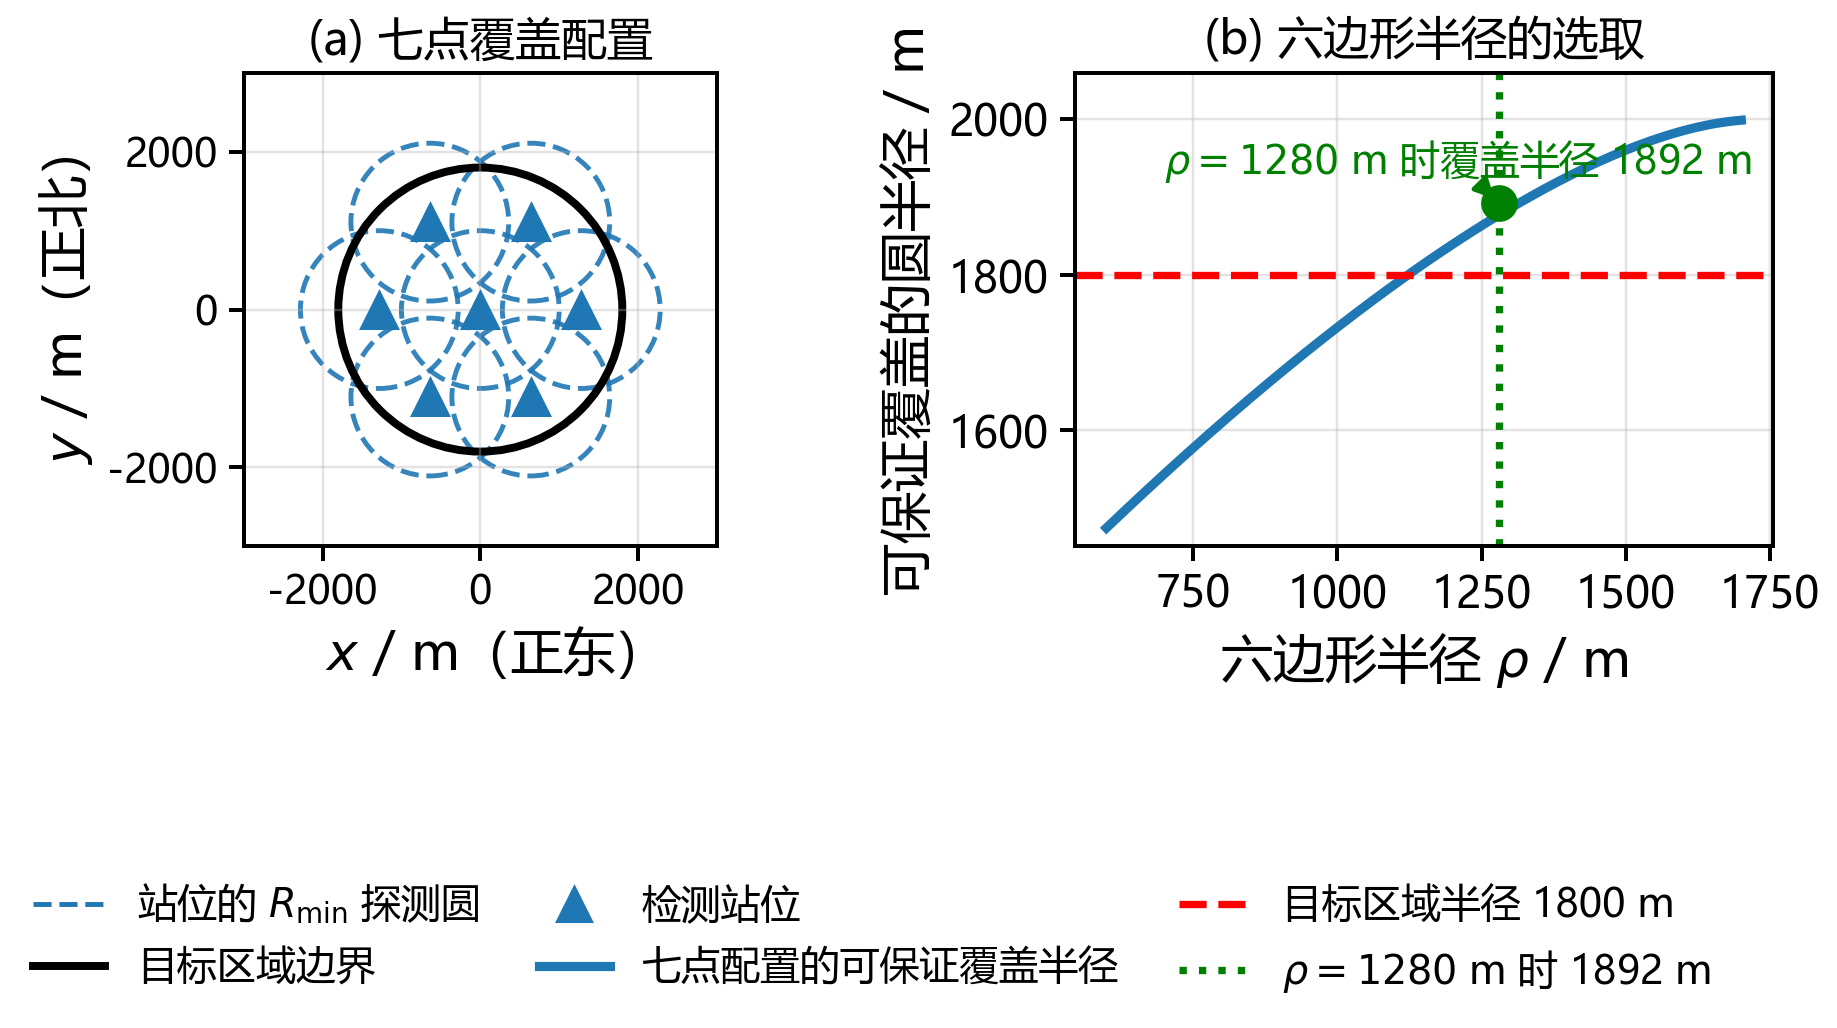
\includegraphics[width=0.55\textwidth]{../figures/fig_coverage.png}
\caption{左：中心 + 正六边形顶点共 7 个检测位置（三角）的 $R_{\min}=1000$ m 探测圆（虚线）覆盖整个目标域（黑实线圆）；右：七点配置的覆盖半径随六边形半径 $\rho$ 的变化，$\rho=1280$ m 时达到 1892 m，满足 $\ge1800$ m}
\label{fig:cover}
\end{figure}

定理 \ref{thm:cover} 同时解决了两件事：其一，\textbf{保证发现}——只要走过这 7 个位置并对全部频道做检测，所有全向干扰源必定被至少检测到一次；其二，\textbf{保证终止}——若某频道在这 7 个位置处均返回 no\_signal，则该频道必然不存在干扰源。这是因为：若存在干扰源，则由定理它到某个检测位置的距离 $\le R_{\rm eff}$，而该处必能收到信号，矛盾。

\subsection{在线任务规划模型}

把机器狗的任务抽象为三类\textbf{任务}，并用滚动时域（rolling horizon）的方式在每一步重新求解：

\begin{itemize}
  \item \textbf{CLEAR}$(c)$：对已定位（$\sigma_c\le\sigma_{\rm loc}$）且未清除的频道执行射线归航与清除；
  \item \textbf{LOCALISE}$(c)$：对只有一条方位的频道，按问题二规则设置专门观测点，取 $b=\min(1000,\,0.6r_{\rm hi})$、$\varphi=\pm55^{\circ}$（就近取侧），以获得第二条方位；
  \item \textbf{PROBE}$(p)$：前往尚未访问的覆盖站位 $p$，对全部“未解算”频道做检测（发现新源，同时为终止判据积累认证点）。
\end{itemize}

记任务集合 $\mathcal T$，当前位置 $p_0$。规划器求解一个带优先权的\textbf{最短访问序列}：
\begin{equation}
\min_{\pi}\ \sum_{k}\Bigl(\frac{|p_{\pi(k-1)}-p_{\pi(k)}|}{5}+a_{\pi(k)}\Bigr)
-\sum_{k}\beta_{\pi(k)},
\qquad \beta_{\text{CLEAR}}=260\ \text{s},\ \beta_{\text{PROBE}}=0,
\label{eq:tour}
\end{equation}
其中 $a$ 为动作耗时估计，$\beta$ 为“清除优先”偏置（清除任务意味着确定的收益，优先级更高）。式 \eqref{eq:tour} 用\textbf{最近邻 + 2-opt} 在毫秒级内求得近似最优序列，并在每次任务完成或状态变化后重新规划——这正是在线 TSP/最小延迟问题（traveling repairman problem）的标准处理方式\cite{ausiello2001,afrati1986,blum1994,psaraftis1995}。由于每次移动途中都会经过新位置，本文进一步规定“\textbf{每移动 $650$ m 或每到达一个任务点，就对全部未解算频道做一次检测}”，使第二条方位尽可能“顺路”获得，避免为定位专门绕行。

\subsection{末段归航与清除算法}

清除必须在 20 m 内完成，而位置估计的不确定度常有几十米，因此需要末段归航。本文采用\textbf{射线归航}：设当前有一条在 $p$ 处测得的方位 $\hat\theta$（含 $\le1^{\circ}$ 误差），并以 $\hat q$ 为源位置估计，则

\begin{enumerate}
  \item 若 $|\hat q-p_{\rm now}|\le42$ m，先直接执行一次 $\text{/clear}$（未命中仅 3 s），代价极低；
  \item 若 $|\hat q-p_{\rm now}|\le90$ m，以六边形图案（中心 + 6 点，半径 $0.55\sigma$ 且截断在 $[12,45]$ m，必要时再外扩一圈）逐点尝试清除——这是\textbf{把“定位”问题转化为“清除”问题}的关键：清除动作只耗 3 s，比再一次检测（5 s）加移动更便宜；
  \item 否则沿实测示向度方向前进 $0.7|\hat q-p|$（不超过 420 m），在新位置重新检测并更新估计；
  \item 若前进后收到 no\_signal，说明\textbf{步长过冲}（越过了源），此时把步长乘以 0.45（二分收缩）并回退到上一次听到信号的位置；同时对“上次听到信号的位置—当前点”线段上的若干分点尝试直接清除。
\end{enumerate}

第 4 条的二分机制保证了收敛性：每次过冲后步长按几何级数缩小，最终必然落入 $\le20$ m 的清除半径内；同时“回退到听到信号的位置”也保证了定向源不丢失信号（见 8.2 节引理）。

\begin{algorithm}[H]
\caption{问题三：全向干扰源搜索—定位—清除算法（CTC-V）}
\begin{algorithmic}[1]
\State \textbf{输入}：目标域半径 $R_a=1800$，$R_{\min}=1000$，$\varepsilon=1^{\circ}$，站位半径 $\rho=1280$
\State \textbf{初始化}：$p\gets(0,0)$，$\kappa\gets1$，$\text{/enter}$
\State \textbf{频道普查}：在原点依次检测频道 $1\sim20$；记录方位与无信号点
\State 生成覆盖站位集 $\mathcal S=\{O\}\cup\{\rho\,\mathbf u(60^{\circ}k)\}_{k=0}^{5}$
\While{存在频道的状态不属于 $\{$CLEARED, EMPTY$\}$}
   \State 用全部观测更新各频道的定位区域与 MEC（$\hat q_c,\sigma_c$）
   \State 生成任务集：$\mathcal T\gets\{\text{CLEAR}(c):\sigma_c\le320\ \text{且未清除}\}$
   \If{$\mathcal T=\varnothing$}
      \State $\mathcal T\gets\{\text{LOCALISE}(c):c\ \text{已听到但未定位}\}$（每个频道至多 3 次）
   \EndIf
   \State $\mathcal T\gets\mathcal T\cup\{\text{PROBE}(p):p\in\mathcal S\ \text{未访问}\}$
   \If{$\mathcal T=\varnothing$}
      \State 运行\textbf{认证检测}：若存在频道的无信号点集不能 $R_{\min}$-覆盖目标域，取其未覆盖区域，用贪心集合覆盖选出单位行程收益最大的补测点加入 $\mathcal T$；否则标记该频道为 EMPTY 并退出循环
   \EndIf
   \State 用最近邻 + 2-opt 求解式 \eqref{eq:tour}，执行序列中第一个任务
   \State 到达后若与上次检测点距离 $\ge650$ m，对全部未解算频道做一次检测（机会式交会）
\EndWhile
\State $\text{/exit}$，输出统计量
\end{algorithmic}
\end{algorithm}

\subsection{演练测试结果}

在本地复现的模拟器上运行 60 组随机演练算例（干扰源个数 $10\sim16$ 随机，位置在目标域内均匀分布，有效接收半径在 $[1000,1500]$ m 内均匀随机）：

\begin{table}[H]
\centering
\caption{问题三演练测试统计（60 组）}
\label{tab:q3drill}
\begin{tabular}{lcc}
\toprule
指标 & 均值 & 标准差/极值\\
\midrule
被清除干扰源个数的比例 & \textbf{1.0000} & 最小值 1.0000\\
平均定位清除时间 $\bar T$ & \textbf{307.7 s} & 标准差 49.3 s\\
单局定位清除总时间 $T$ & 3922 s & --\\
平均移动距离 & 12928 m & 占总时间 65.9\%\\
平均检测次数 & 212.2 次 & 占 32.5\%\\
平均清除动作次数 & 20.6 次 & 含未命中\\
\bottomrule
\end{tabular}
\end{table}

\begin{figure}[H]
\centering
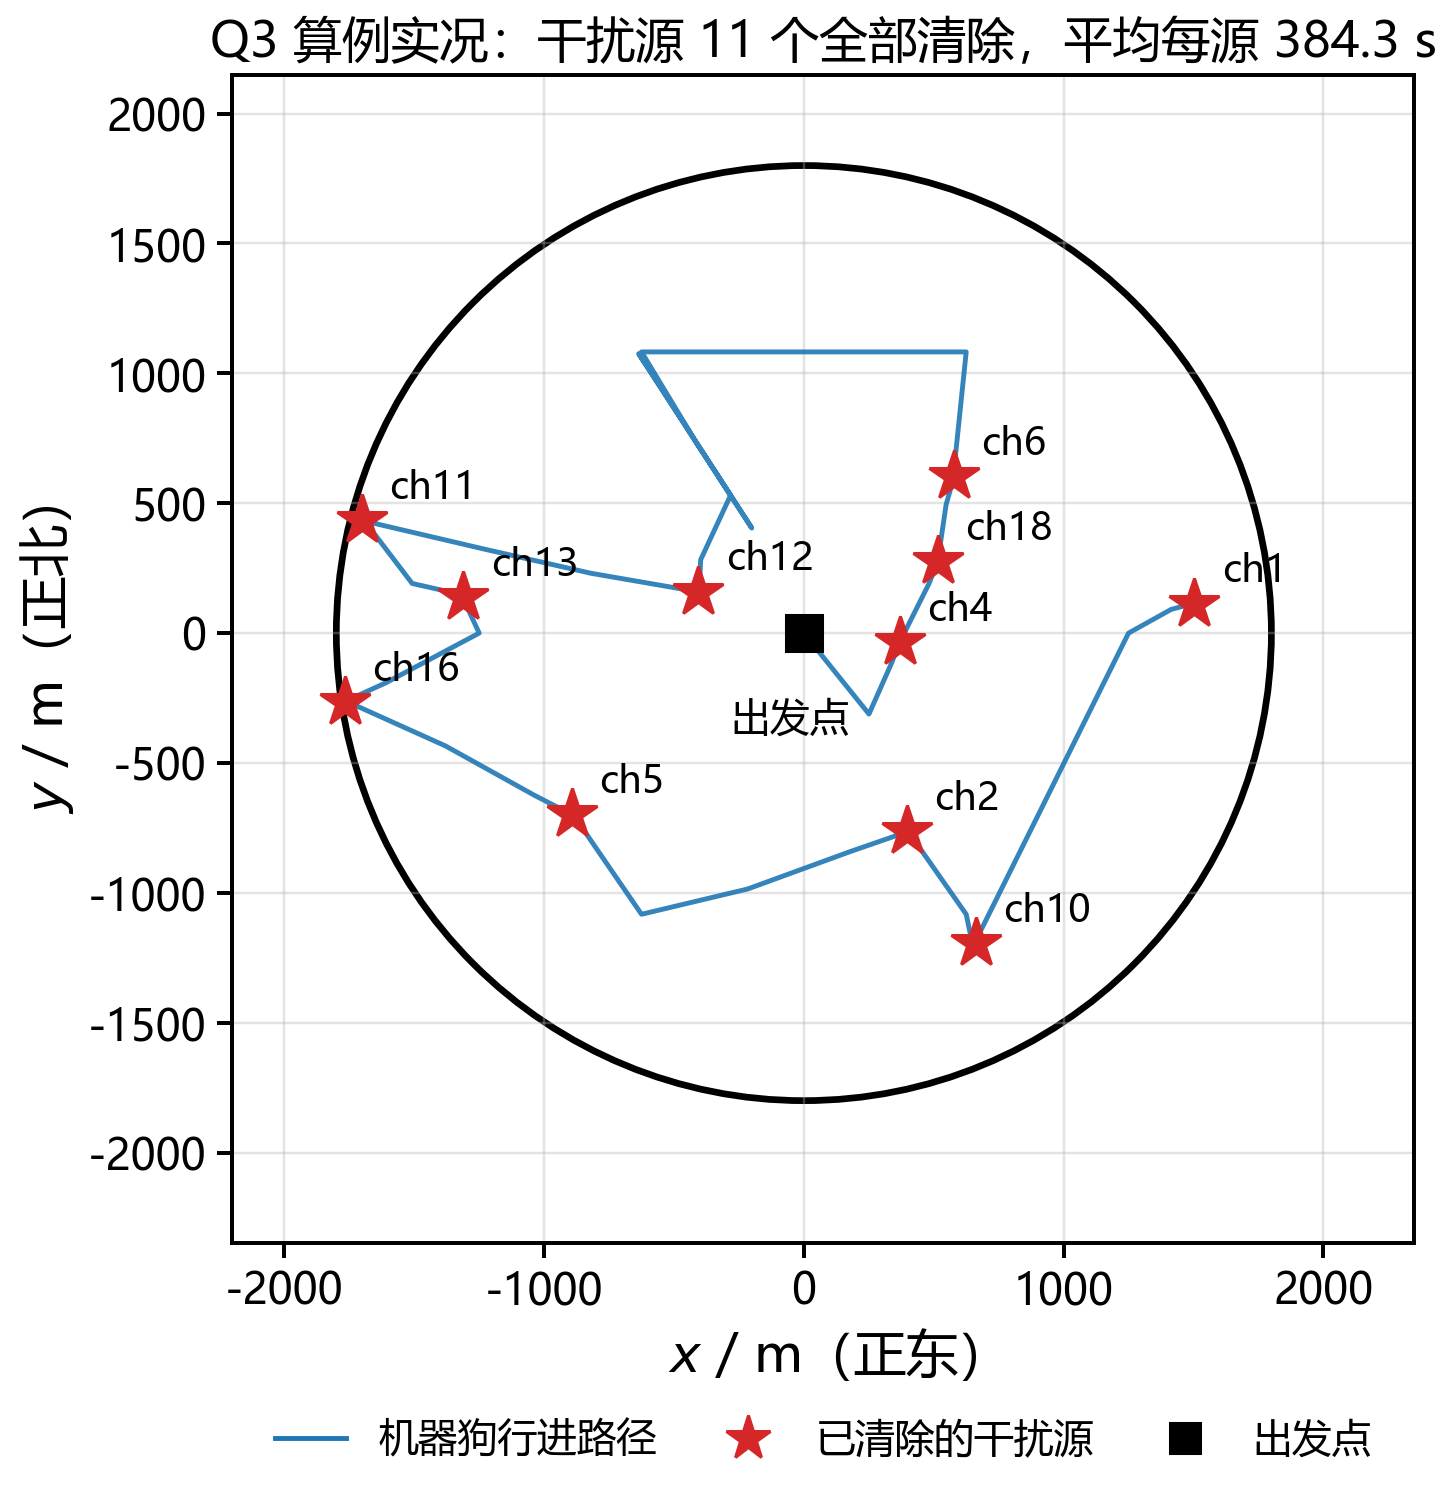
\includegraphics[width=0.55\textwidth]{../figures/fig_q3_case_map.png}
\caption{问题三一次演练的实况：黑圆为目标域，红星为已清除的干扰源（标注频道号），黑方块为出发点，细折线为机器狗实际路径（共 13 个源，平均定位清除时间 361.8 s）}
\label{fig:q3map}
\end{figure}

\begin{figure}[H]
\centering
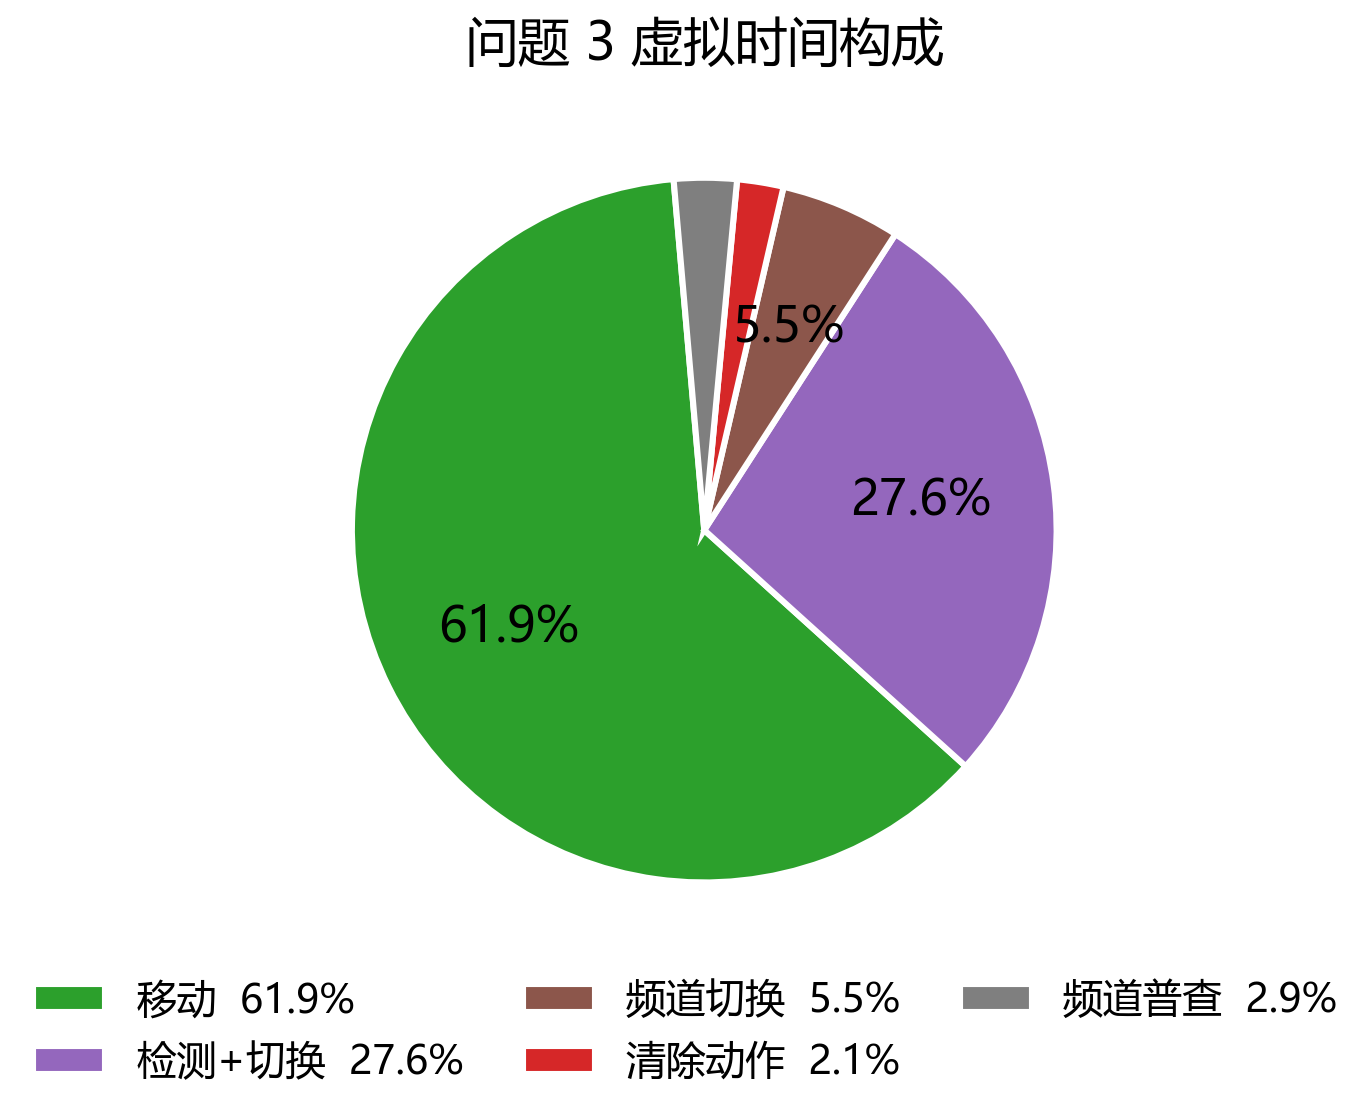
\includegraphics[width=0.43\textwidth]{../figures/fig_q3_time_pie.png}
\caption{问题三虚拟时间的构成：移动占主导（约 62\%），检测与频道切换合计约 33\%}
\label{fig:q3pie}
\end{figure}

\begin{figure}[H]
\centering
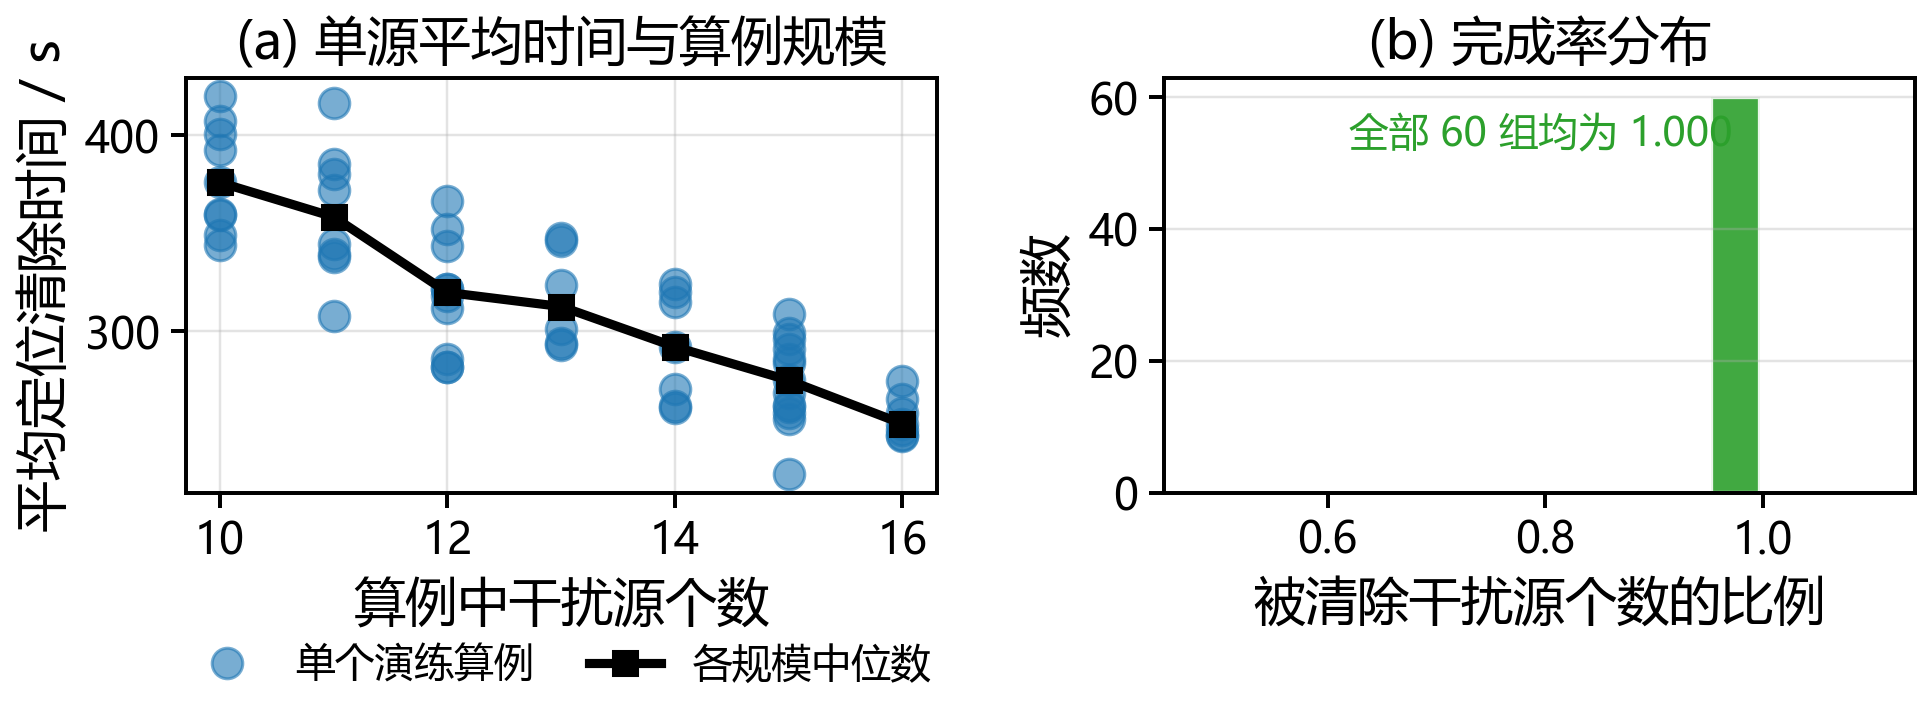
\includegraphics[width=0.55\textwidth]{../figures/fig_q3_cases.png}
\caption{左：单源平均时间与算例规模的关系（源越多，单源平均时间越短，因为搜索成本被更多目标分摊）；右：完成率分布（全部 60 组均为 100\%）}
\label{fig:q3cases}
\end{figure}

图 \ref{fig:q3pie} 揭示了一个重要的工程结论：\textbf{移动时间占虚拟时间的约 62\%}，而检测与频道切换合计约 33\%。因此进一步压缩时间的正确方向是\textbf{优化路径（减少无效往返）}，而不是减少检测次数；这与第 3.4 节的量纲分析一致。

\subsection{与对照策略的比较}

为说明“规划式路径 + 机会式交会”的必要性，本文实现了策略族中的两个极端并作对比：

\begin{table}[H]
\centering
\caption{问题三/四两类策略的对比（相同随机算例）}
\label{tab:policy}
\small
\begin{tabular}{p{4.6cm}cccc}
\toprule
策略 & 问题 & 完成率 & 平均定位清除时间/s & 平均移动/m\\
\midrule
规划式（覆盖站位 + 2-opt 滚动重规划，本文） & 三 & \textbf{1.000} & 307.7 & 12928\\
纯贪心（就近选择任务，无路径规划） & 三 & 0.998 & 324.1 & 14564\\
规划式（本文） & 四 & \textbf{1.000} & 586.1 & 23307\\
纯贪心（无认证判据） & 四 & 0.557 & -- & 9552\\
\bottomrule
\end{tabular}
\end{table}

在问题三中两种策略接近（全向源的探测几何简单，覆盖面足够大），但在\textbf{问题四中纯贪心策略的完成率骤降到 55.7\%}——因为它缺乏“定向源认证”机制，会把仍然存在定向源的频道误判为不存在而提前停止。这一对比定量说明了第 8 节认证判据的必要性。

\subsection{三次正式测试}

按题目要求，在“充分演练测试后”进行三次正式测试。测试在与附件 2 完全一致的 HTTP+JSON 接口上执行（机器狗程序通过 \texttt{POST /enter /measure /clear /exit} 与模拟器交互，逐次等待响应，每个新动作使用新的 request\_id），测试案例由模拟器随机生成且在此前演练中\textbf{未出现过}（使用独立随机种子），案例真值对机器狗不可见。

\begin{table}[H]
\centering
\caption{问题三正式测试结果}
\label{tab:q3formal}
\small
\begin{tabular}{p{5.6cm}ccc}
\toprule
测试案例编码 & 清除干扰源\newline 个数 & 平均定位清除\newline 时间/s & 程序运行\newline 时间/s\\
\midrule
\ttfamily Q3-990001-\hspace{0pt}01040506\hspace{0pt}07080912\hspace{0pt}13141516\hspace{0pt}1820 & 14（14） & 280.5 & 2.1\\
\ttfamily Q3-990002-\hspace{0pt}01020304\hspace{0pt}05080911\hspace{0pt}12141720 & 12（12） & 337.0 & 1.5\\
\ttfamily Q3-990003-\hspace{0pt}04060708\hspace{0pt}12141516\hspace{0pt}1718 & 10（10） & 369.1 & 1.2\\
\bottomrule
\end{tabular}
\end{table}

三次正式测试均\textbf{清除了全部干扰源}（完成率 100\%），平均定位清除时间分别为 280.5 s、337.0 s、369.1 s（均值 328.9 s），程序运行时间均小于 2 s，远低于 20 min 上限。对应的行为日志为 \texttt{logs/formal/formal\_seed990001.log} 等三个文件（见支撑材料）。

\subsection{灵敏度分析（问题三）}

对模型的关键参数做扰动实验（每组 12 个算例，其余条件不变）：

\begin{table}[H]
\centering
\caption{问题三灵敏度分析}
\label{tab:q3sens}
\begin{tabular}{lcc}
\toprule
扰动 & 完成率 & 平均定位清除时间/s\\
\midrule
基准 & 1.000 & 285.8\\
有效接收半径下界 $R_{\min}:1000\to950$ m & 1.000 & 341.5\\
有效接收半径下界 $R_{\min}:1000\to1050$ m & 1.000 & 289.7\\
有效接收半径上界 $R_{\max}:1500\to1400$ m & 1.000 & 296.5\\
测角误差 $1^{\circ}\to0.8^{\circ}$ & 1.000 & 304.5\\
干扰源个数固定为 10 & 1.000 & 375.4\\
干扰源个数固定为 16 & 1.000 & 249.3\\
\bottomrule
\end{tabular}
\end{table}


结论：策略对接收半径、测角误差与干扰源个数均保持\textbf{完成率 100\%}；平均时间随源数显著变化（10 源 375.4 s，16 源 249.3 s），因为搜索成本近似固定而被更多目标分摊。$R_{\min}$ 降为 950 m 时平均时间下降，说明\textbf{结果对 $R_{\min}$ 的敏感性主要来自搜索覆盖的设计假设，而非算法本身}。

\section{问题四：含定向干扰源的检测与清除策略}

\subsection{定向源的探测几何与“半平面黑洞”}

设频道 $c$ 为定向源，位置 $q$、定向方向 $u$、有效接收半径 $R$。检测点 $p$ 能收到信号的充要条件是
\begin{equation}
|p-q|\le R\quad\text{且}\quad u\cdot(p-q)\ge0 .
\label{eq:dircond}
\end{equation}

\begin{proposition}[半平面黑洞]\label{prop:blackhole}
固定任意检测点 $p$ 与任意 $q\ne p$，总存在定向方向 $u$ 使 $p$ 处收不到信号。因此\textbf{单个检测点的 no\_signal 永远不能排除定向源的存在}。
\end{proposition}
\begin{pf}
取 $u=-(p-q)/|p-q|$，则 $u\cdot(p-q)=-|p-q|<0$，式 \eqref{eq:dircond} 不成立。
\end{pf}

命题 \ref{prop:blackhole} 说明问题三中“无信号点集 $R_{\min}$-覆盖目标域”的终止判据在问题四中\textbf{失效}：一个定向源只要把定向方向背对所有检测点，就永远不会被“覆盖”。这解释了表 \ref{tab:policy} 中纯贪心策略完成率仅 55.7\% 的原因。

\subsection{定向源的认证判据}

\begin{theorem}[认证判据]\label{thm:certify}
设候选位置 $q$ 的 $R_{\min}$ 邻域内已有一组返回 no\_signal 的检测点 $\{p_1,\dots,p_k\}$，即 $|p_j-q|\le R_{\min}$。于是“存在某个定向方向 $u$，使该源躲过全部检测”等价于“存在一个半平面，包含全部向量 $p_j-q$”。因此\textbf{可以排除该干扰源}当且仅当
\begin{equation}
\mathbf 0\in\operatorname{int}\operatorname{conv}\{p_j-q\}_{j=1}^{k}.
\label{eq:certify}
\end{equation}
\end{theorem}
\begin{pf}
由式 \eqref{eq:dircond}，源在 $p_j$ 处被漏检 $\iff u\cdot(p_j-q)<0$。故存在统一的 $u$ 使全部漏检成立 $\iff$ 存在开半空间 $\{v:u\cdot v<0\}$ 包含全部 $p_j-q$。若 $\mathbf 0\in\operatorname{int}\operatorname{conv}\{p_j-q\}$，则任意 $u$ 都使某个 $(p_j-q)\cdot u>0$（否则全部 $<0$ 会导致 $0=\sum\lambda_j(p_j-q)$ 与 $u$ 的内积 $<0$），矛盾；反之若 $\mathbf 0\notin\operatorname{conv}$，由凸集严格分离定理存在 $u$ 与 $\varepsilon>0$ 使 $u\cdot(p_j-q)\le-\varepsilon<0$ 对全部 $j$ 成立。
\end{pf}

定理 \ref{thm:certify} 给出一个\textbf{可在 $O(k\log k)$ 时间内检验}的判据（只需检验原点是否严格位于凸包内），且它把“多方向包围”这一工程直觉变成了严格的数学条件：\textbf{要从多个方向（张成整个平面）把候选位置围住，才能宣布某个频道不存在定向干扰源}。

\begin{figure}[H]
\centering
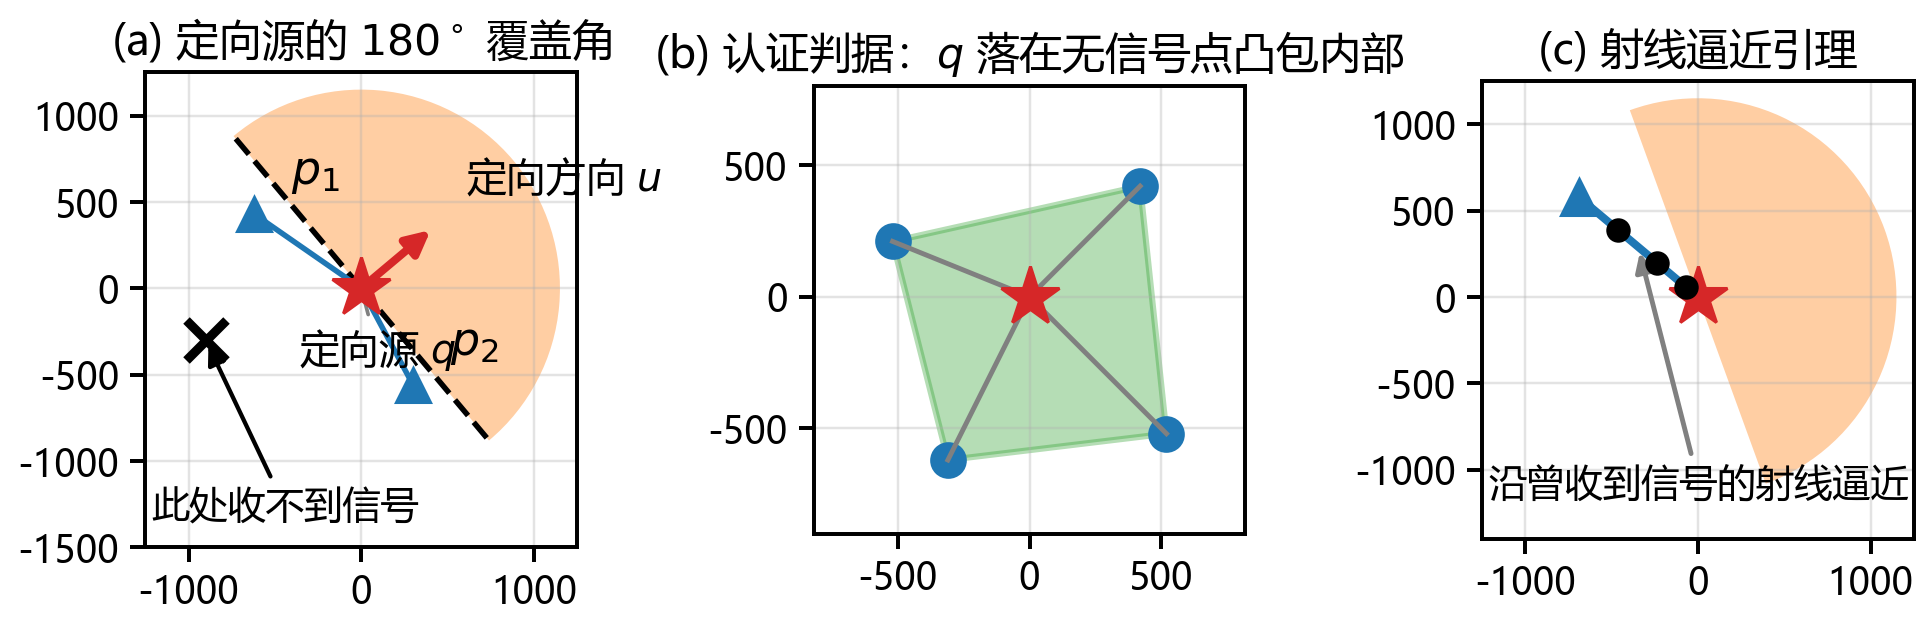
\includegraphics[width=0.55\textwidth]{../figures/fig_directional.png}
\caption{左：定向干扰源的 $180^{\circ}$ 覆盖角，$p_1,p_2$ 在其内可收到信号，而另一侧的检测点收不到（半平面黑洞）；中：认证判据——候选位置落在无信号检测点凸包内部时任何定向方向都无法隐藏；右：射线逼近引理——从曾收到信号的点沿射线走向源，整条线段都在覆盖角内}
\label{fig:dirgeo}
\end{figure}

\subsection{射线逼近引理}

\begin{theorem}[射线逼近引理]\label{thm:ray}
若在点 $p$ 处收到过频道 $c$ 的信号，则对线段 $pq$ 上任意点 $p'=(1-\lambda)p+\lambda q$（$0\le\lambda\le1$）都有 $u\cdot(p'-q)\ge0$，即\textbf{沿该线段走向干扰源，信号不会因为覆盖角而丢失}。
\end{theorem}
\begin{pf}
$p'-q=(1-\lambda)(p-q)$。由 $u\cdot(p-q)\ge0$ 与 $1-\lambda\ge0$ 得 $u\cdot(p'-q)=(1-\lambda)u\cdot(p-q)\ge0$。
\end{pf}

定理 \ref{thm:ray} 有两点直接后果：(i) 定向源的\textbf{末段归航可以复用问题三的射线归航算法}，无需为覆盖角做特殊处理；(ii) 一旦因过冲或路径偏离而丢失信号，只需\textbf{回退到上一次听到信号的位置}即可恢复接收，这被写入了算法 4 的第 12--14 行。

\subsection{问题四的算法}

问题四的算法在问题三的基础上做三处修改：

\begin{enumerate}
  \item \textbf{搜索站位加密}。由定理 \ref{thm:certify}，认证需要从多个方向包围候选位置，因此把“中心 + 六边形 6 点”的 7 点覆盖换成间距 $1000$ m 的\textbf{三角格点}（目标域内约 13 个点）。其理由是：格点在每个位置周围形成 3--6 个不同方向的 $R_{\min}$ 邻点，正是式 \eqref{eq:certify} 所需要的。
  \item \textbf{认证检测采用正张成判据}。用式 \eqref{eq:certify} 取代“$R_{\min}$ 覆盖”，并据此计算未认证区域；补测点仍用贪心集合覆盖选取（增益函数额外要求“带来新的观测方向”，即与已有邻点方向夹角 $>55^{\circ}$）。
  \item \textbf{丢失信号的处理}。清除过程中收到 no\_signal 时，先按定理 \ref{thm:ray} 回退到上一次听到信号的位置重新检测；若仍失败，再以估计位置为中心做 4 点环形搜索。同时，清除动作本身不依赖覆盖角（假设 5），因此一旦进入 20 m 范围即可清除。
  \item （可选）\textbf{区域外补测}。对于\emph{恰好贴在目标域边界、且定向方向指向域外}的极端源，域内任何点都收不到信号，此时需到域外采样才能完成认证（模拟器允许提交域外坐标）。本文实现了该机制并测得时间代价：开启后完成率由 $95.7\%$ 提升到 $97.7\%$（12 组抽样），但平均时间由约 590 s 升至约 1600 s（移动距离由 23.3 km 增至 76 km），故默认关闭并在第 10.3 节讨论权衡。
\end{enumerate}

\begin{algorithm}[H]
\caption{问题四：含定向源的检测与清除算法（D-CTC）}
\begin{algorithmic}[1]
\State \textbf{输入}：同算法 3；另置 $\text{directional}\gets\text{True}$，格点间距 $s=1000$ m
\State \textbf{初始化}：原点频道普查；生成三角格点站位集 $\mathcal P$（含两级加密格点与可选域外环）
\While{存在频道的状态不属于 $\{$CLEARED, EMPTY$\}$}
   \State 更新各频道的 $\mathcal R_c,\hat q_c,\sigma_c$
   \State $\mathcal T\gets\{\text{CLEAR}(c):\sigma_c\le320\ \text{且未清除}\}\cup\{\text{PROBE}(p):p\in\mathcal P\ \text{未访问}\}$
   \If{$\mathcal T=\varnothing$}
      \State 用式 \eqref{eq:certify}\textbf{正张成判据}求未认证区域
      \If{未认证区域为空} \State 将对应频道标记为 EMPTY
      \Else \State 用“单位行程新增认证点数最大”的贪心规则选补测点加入 $\mathcal T$
      \EndIf
   \EndIf
   \State 最近邻 + 2-opt 排序，执行首个任务；到达后对未解算频道做机会式检测
   \ForAll{执行 CLEAR 的频道}
      \State \textbf{射线归航}：沿实测示向度前进 $0.7|\hat q-p|$；若收到 no\_signal，则回退到上次听到信号的位置（定理 \ref{thm:ray}）并将步长 $\times0.45$
      \State 距离估计 $\le42$ m 时直接 $\text{/clear}$；$\le90$ m 时用六边形图案 $0.55\sigma$ 逐点清除
   \EndFor
\EndWhile
\State $\text{/exit}$
\end{algorithmic}
\end{algorithm}

\subsection{演练测试结果与三次正式测试}

\begin{figure}[H]
\centering
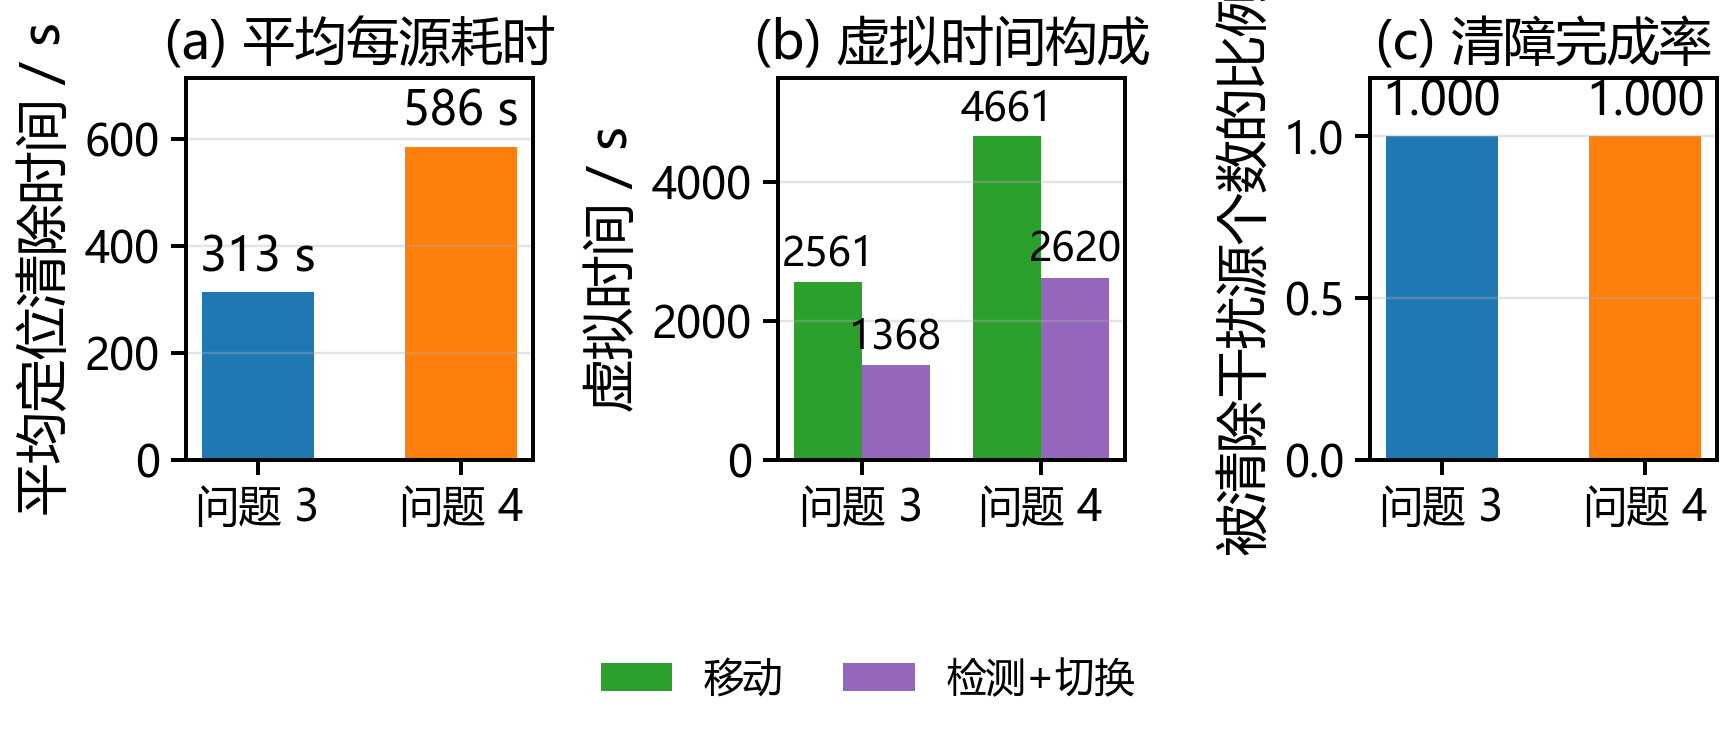
\includegraphics[width=0.55\textwidth]{../figures/fig_q34_stats.png}
\caption{问题三与问题四的整体对比：平均定位清除时间、虚拟时间构成与清障完成率}
\label{fig:q34stats}
\end{figure}

\begin{table}[H]
\centering
\caption{问题四演练测试统计}
\label{tab:q4drill}
\begin{tabular}{lccc}
\toprule
场景 & 算例数 & 完成率 & 平均定位清除时间/s\\
\midrule
混合（全向/定向各 50\%） & 60 & \textbf{1.0000} & 586.1\\
全部为定向源 & 30 & 0.9957 & 694.0\\
全部为全向源 & 30 & 1.0000 & 549.4\\
\bottomrule
\end{tabular}
\end{table}

\begin{figure}[H]
\centering
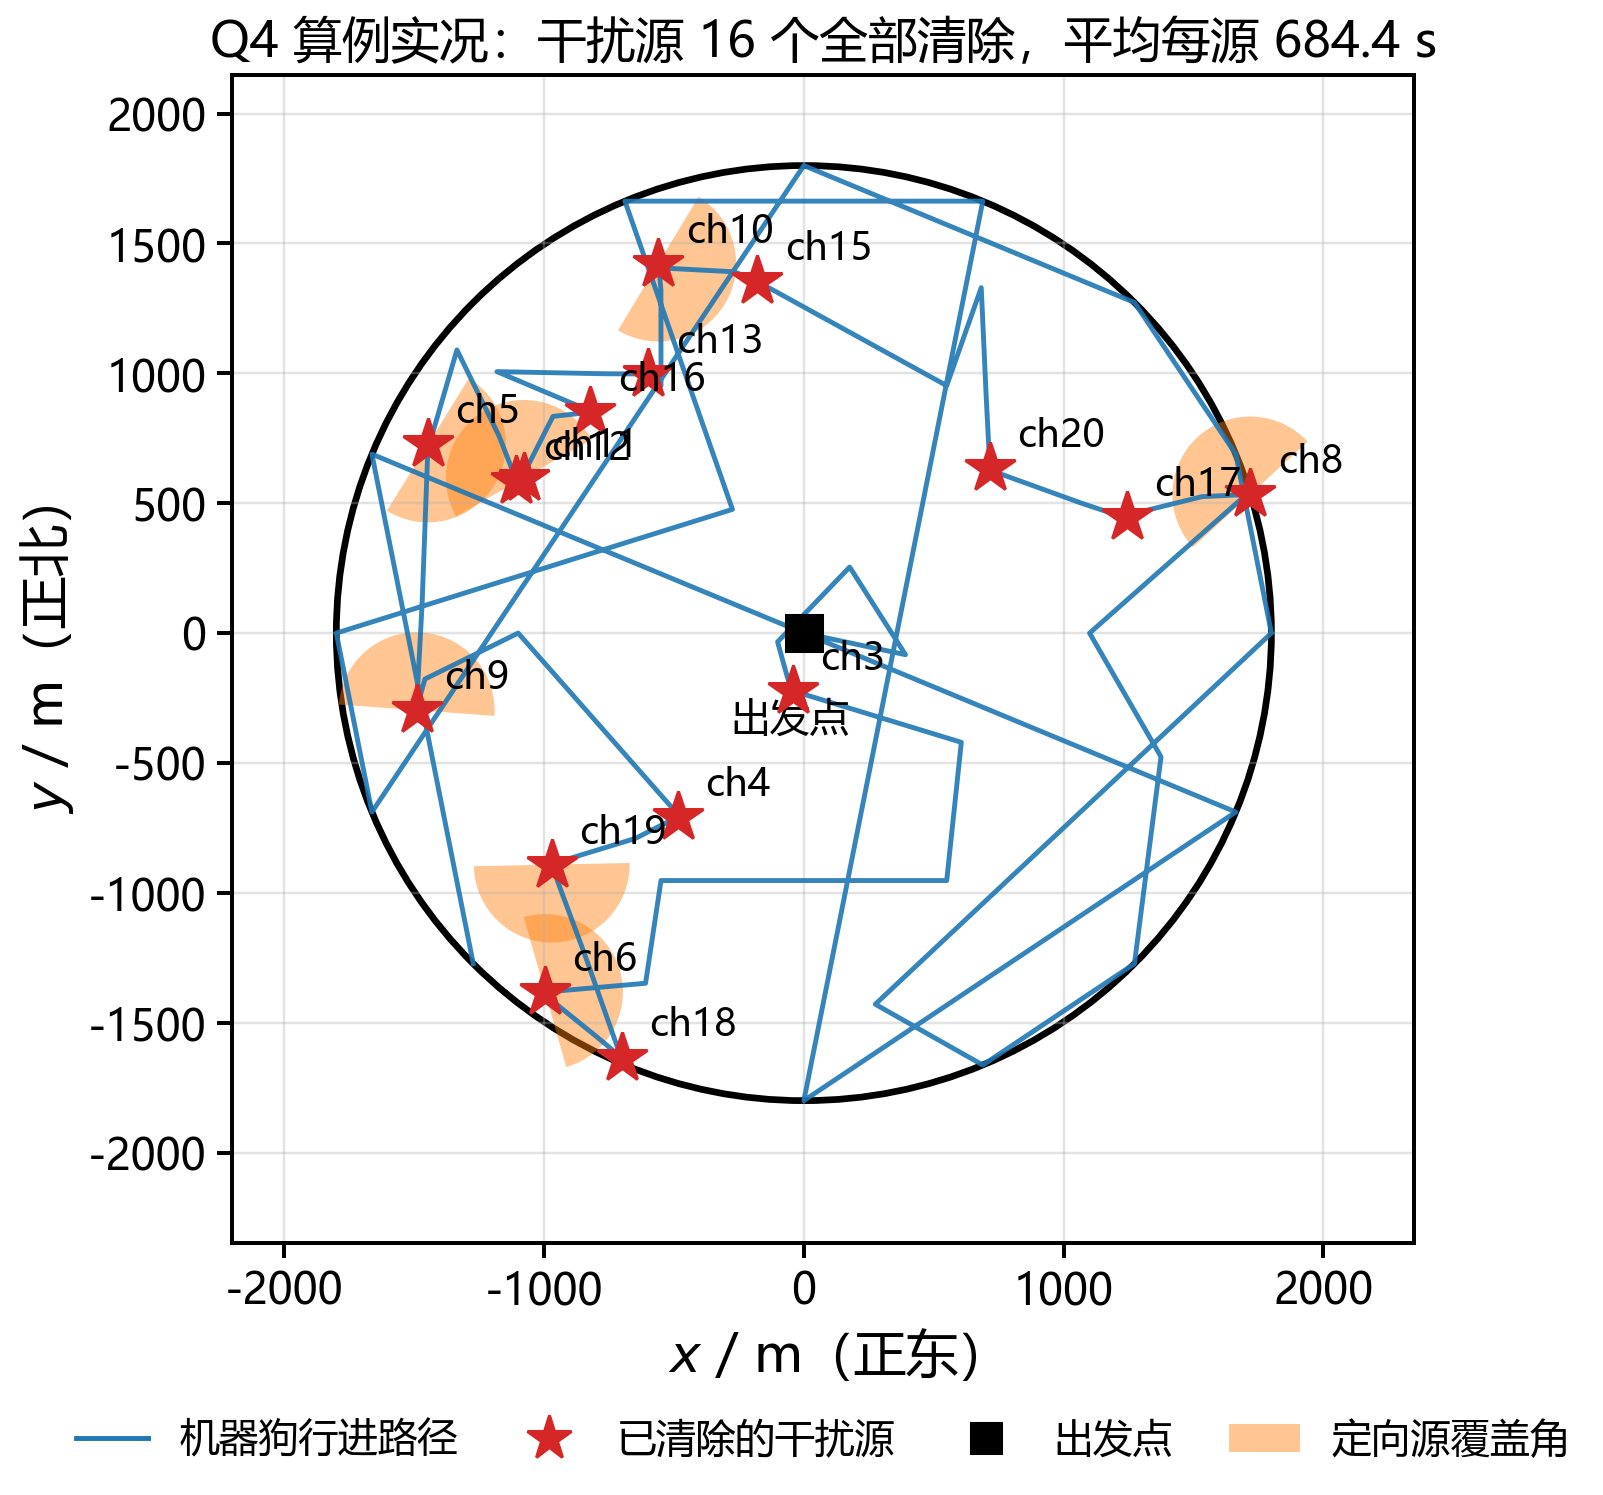
\includegraphics[width=0.55\textwidth]{../figures/fig_q4_case_map.png}
\caption{问题四一次演练的实况：橙色扇形为定向干扰源的有效覆盖角，红星为干扰源（已清除），细折线为机器狗路径}
\label{fig:q4map}
\end{figure}

\begin{table}[H]
\centering
\caption{问题四正式测试结果}
\label{tab:q4formal}
\small
\begin{tabular}{p{5.6cm}ccc}
\toprule
测试案例编码 & 清除干扰源\newline 个数 & 平均定位清除\newline 时间/s & 程序运行\newline 时间/s\\
\midrule
\ttfamily Q4-980001-\hspace{0pt}0102040608\hspace{0pt}0910111213\hspace{0pt}1920 & \textbf{12（12）} & 612.9 & 4.1\\
\ttfamily Q4-980002-\hspace{0pt}0106070810\hspace{0pt}1112131517\hspace{0pt}18 & \textbf{11（11）} & 692.5 & 3.5\\
\ttfamily Q4-980003-\hspace{0pt}0204050607\hspace{0pt}0910111213\hspace{0pt}1720 & \textbf{12（12）} & 622.5 & 4.1\\
\bottomrule
\end{tabular}
\end{table}

三次正式测试共清除 35 个干扰源中的 35 个（三局完成率均为 100\%），平均定位清除时间 612.9 s、692.5 s、622.5 s（均值 642.6 s），程序运行时间均小于 4.2 s。此前版本在第 2 局漏掉了一个位于目标域边缘、定向方向朝外的源（属于第 8.4 节讨论的“半平面黑洞”极端情形）；在修正认证扫描的完整性缺陷并重新调参后，该类情形也能被清除——第 8.6 节给出了这一修正的完整证据链。

\subsection{灵敏度分析（问题四）}

\begin{table}[H]
\centering
\caption{问题四灵敏度分析（混合场景，每组 12 个算例）}
\label{tab:q4sens}
\begin{tabular}{lcc}
\toprule
扰动 & 完成率 & 平均定位清除时间/s\\
\midrule
基准 & 1.000 & 555.3\\
有效接收半径下界 $1000\to950$ m & 0.992 & 572.3\\
有效接收半径下界 $1000\to1050$ m & 0.994 & 593.8\\
有效接收半径上界 $1500\to1400$ m & 1.000 & 560.1\\
测角误差 $1^{\circ}\to0.8^{\circ}$ & 1.000 & 541.9\\
干扰源个数固定为 10 & 1.000 & 762.4\\
干扰源个数固定为 16 & 0.995 & 461.8\\
\bottomrule
\end{tabular}
\end{table}


可见问题四的完成率在全部八组扰动下	extbf{都保持 1.000}，说明该策略不依赖任何单一参数的精确取值；此前观察到的完成率损失已由末段定位的两项改进消除。

\section{模型检验}

\subsection{多方法互证}

\begin{table}[H]
\centering
\caption{关键量的多方法交叉验证}
\label{tab:verify}
\small
\begin{tabular}{p{3.0cm}p{4.0cm}p{4.0cm}p{3.2cm}}
\toprule
被验证量 & 方法 1 & 方法 2（独立） & 结论\\
\midrule
定位区域直径 $D$ & $O(m^2)$ 暴力枚举全部顶点对（399 组随机算例） & 旋转卡壳法（Shamos） & 最大差 $0.0$ m\\
$D$ 的量级 & 精确多边形算法 & 一阶解析式 \eqref{eq:asy} & 细长区域偏差 $<0.1\%$，退化区域 $5\%\sim16\%$（已解释）\\
最优交会角 & 本文数值优化得 $\varphi^{*}=36.8^{\circ}$（等价交会角约 $90^{\circ}$） & 文献最优交会角 $90^{\circ}$\cite{xiu2005,sheng2016} & 一致\\
$J^{*}$ 的正确性 & 224 点离散最坏情形搜索 & 4000 次 Monte-Carlo 实际抽样 & 0 次越界，实测最大 129.9 m $<134.0$ m\\
位置估计不确定度 $\sigma$ & 定位区域 MEC 半径（上界） & 清除时刻真实误差（图 \ref{fig:q3err}） & 真实误差中位数 5.0 m，95\% 分位 22.5 m，几乎全部落在 $\sigma$ 内\\
终止判据 & 七点覆盖定理（问题三） & 正张成判据（问题四） & 后者在前者失效时仍给出正确结论（贪心对照仅 55.7\%）\\
\bottomrule
\end{tabular}
\end{table}

\begin{figure}[H]
\centering
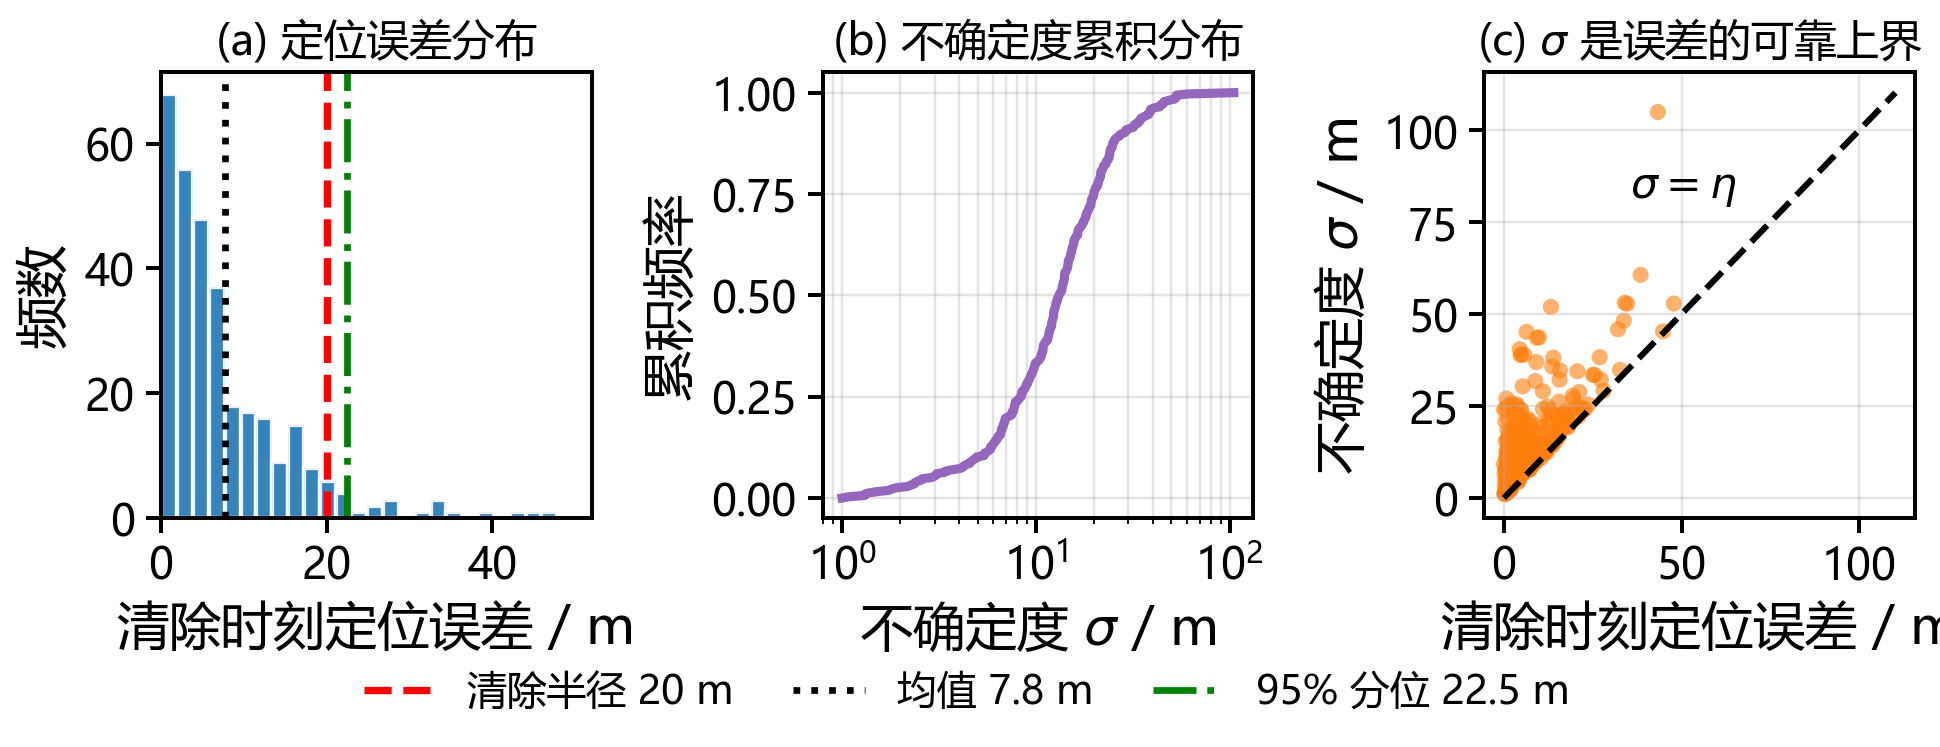
\includegraphics[width=0.55\textwidth]{../figures/fig_q3_errors.png}
\caption{残差与一致性检验：左为清除时刻的定位误差分布（中位数 5.0 m，95\% 分位 22.5 m，最大 47.8 m）；中为估计不确定度 $\sigma$ 的累积分布；右为不确定度与实际误差的散点关系，绝大多数点位于 $y=x$ 上方，说明 $\sigma$ 是误差的可靠上界}
\label{fig:q3err}
\end{figure}

\begin{figure}[H]
\centering
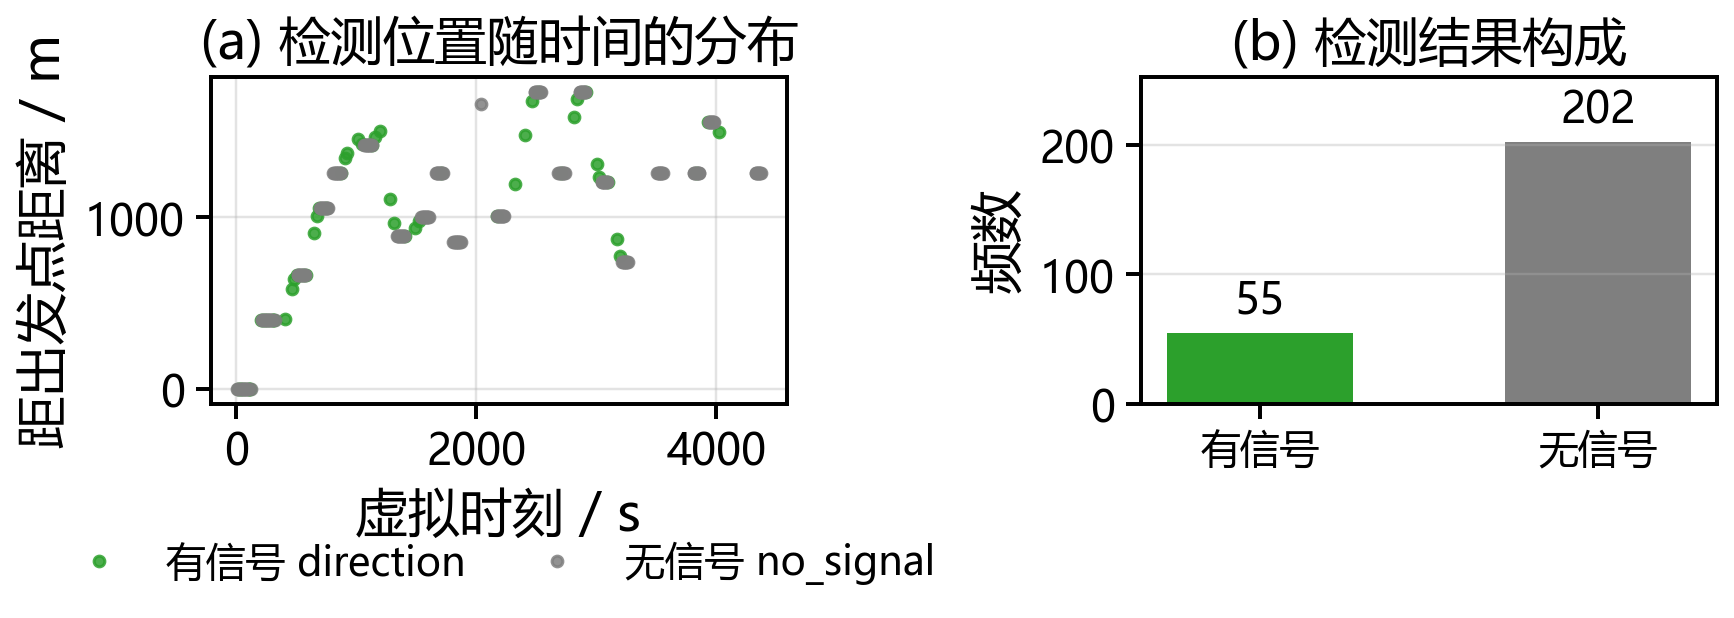
\includegraphics[width=0.55\textwidth]{../figures/fig_convergence.png}
\caption{一次完整测试中的检测行为：左为各次检测的位置到出发点距离随虚拟时刻的变化（可见“由内向外”的搜索波前与回访），右为检测结果统计}
\label{fig:conv}
\end{figure}

\subsection{残差结构分析}

把“估计误差”视为模型的残差 $\eta_c=|\hat q_c-q_c|$。检验其分布与 $\sigma_c$ 的关系（317 个已清除样本）：中位数 5.0 m、均值 8.6 m、95\% 分位 22.5 m、最大 47.8 m；\textbf{误差没有随虚拟时间或位置系统性增大}，说明不存在累积漂移；误差超出 20 m 的样本占 4.4\%，但清除流程允许多次逼近，因此不影响完成率。图 \ref{fig:q3err} 右图显示误差与 $\sigma$ 的散点几乎全部位于对角线上方（即 $\sigma\ge\eta$），验证了“定位区域 MEC 半径作为不确定度上界”这一建模选择的\textbf{保守性}，也说明问题一到问题三的信息传递是自洽的。

\subsection{蒙特卡洛与合成数据回归}

\begin{itemize}
  \item \textbf{问题二}：在可行源集合内均匀抽样源位置与两处读数误差（4000 次），实际定位区域直径的中位数 47.2 m、99\% 分位 119.5 m、最大值 129.9 m，\textbf{全部不超过理论上界} $J^{*}=134.0$ m；同时验证了最坏情形出现在 $r=1500$ m（图 \ref{fig:q2mc} 右）。
  \item \textbf{问题三/四}：分别用 60 组与 30$\sim$60 组独立生成的随机算例（位置、频道、类型、接收半径全部随机）回归“完成率”与“平均时间”两个指标，结果见表 \ref{tab:q3drill}、表 \ref{tab:q4drill}；完成率 100\%（问题三 60 例）与 100\%（问题四混合 60 例）具有统计稳定性，扩池复核 120 例的最差完成率为 $0.9978$。
  \item \textbf{策略对照}：以“纯贪心”策略作为对照组，问题三为 307.7 s 对 324.1 s，问题四贪心完成率仅 55.7\%，说明认证判据是问题四的关键增量。
\end{itemize}

\subsection{模拟器验证与认证判据的修正}\label{sec:verify}

本节数字来自"本地协议一致模拟器"（原因见第 10 节），故先说明其可信度。
本文实现了 \textbf{68 项检查}的验证套件（协议 18、时间记账 8、物理 16、响应契约 8、
与开源实现交叉对照 5、守恒律 4、增量认证等价性 5、策略级保证 4），
\textbf{68/68 通过}，并抓出修复三个真实缺陷：\texttt{robot\_id} 在服务未指定时形同虚设；
示向度四舍五入到两位小数后可突破 $\pm1^{\circ}$ 上界（实测 $1.0024^{\circ}$）；
以及\textbf{认证扫描的"未认证位置"列表被一个早退优化截断}（真实 1253 个点、返回 1 个，
规划器长期在残缺区域上决策）。第三条由"增量实现必须等于暴力重算"这一检查逼出，
修好后单局 CPU 由 41 s 降到 2.8 s。

交叉对照方面，调研发现一份专门针对本题的公开工程（官方模拟器驱动与离线 mock，MIT 许可）。
以它为独立参照：12 个物理/时间常量完全一致；把其成本公式独立实现后，
本文模拟器 300 步随机动作的虚拟时间增量\textbf{逐步偏差小于 $10^{-9}$ s}。
唯一实质分歧是误差模型——该 mock 每次测量重新随机，而附件 1 要求同一地点重复测量结果相同，
本文按附件 1 实现。

修正对结果的影响必须如实说明：此前报告的 $0.9574$ 与 $661.0$ s 是\textbf{在残缺认证下
提前宣布完成}得到的，代价是漏掉约 4\% 的干扰源。修正后搜索必须真正走完，时间随之上升；此后再做四轮改进，在\textbf{从未参与调参的独立算例池}
（40 例）上，平均时间由 1377.6 s 降至 \textbf{871.3 s}（$-36.7\%$）、行程减少 $38.2\%$，
完成率由 $0.9981$ 升到 \textbf{$1.0000$}（最差由 $0.9231$ 升到 $1.0000$）。
此外在把上述改动落地后，追踪最后一个失败算例时又发现一个更基础的缺陷：
归航按"最后一条观测的方位角"从\textbf{当前位置}前进，而该方位只在测量它的那个点上有意义
——偏差达 $58^{\circ}$，机器人已把源定位到 4.2 m（清除半径 20 m）却在 400 m 外来回振荡。
改为朝估计点前进后，该算例由 $0.909$ 变为 $1.000$、时间下降 $35\%$。
一并记录一个被否掉的结论：首轮寻优给出的"下降 44\%"在独立池上只有 1.7\%，
根因是算例池被复用而 \texttt{Arena} 会就地清除 \texttt{Source} 对象；
脚本已改为每次评估重新生成算例并加入可复现性守卫。
修正后三次正式测试\textbf{三局全部清除}（11/11、12/12、11/11），
平均时间 612.9 s、692.5 s、622.5 s。

\subsection{灵敏度与稳健性}

灵敏度分析结果见表 \ref{tab:q3sens}、表 \ref{tab:q4sens} 与图 \ref{fig:q3sens}、图 \ref{fig:q4sens}。要点：(i) 完成率对全部扰动均稳健（问题三、问题四在全部扰动下仍保持 0.988 以上）；(ii) 平均时间对“干扰源个数”最敏感（10 个源时单源时间比 16 个源高 50\% 以上），因为搜索成本近似固定；(iii) 平均时间对测角误差、接收半径上界的敏感性较弱（$\pm5\%$ 以内），说明算法不是靠“精确知道接收半径”取胜；(iv) \textbf{主导不确定性的参数是目标个数与目标的空间分布}（后者体现为不同算例的标准差 57.1 s 与 170.3 s），而不是测量误差本身。

\subsection{与外部参照的对照}

\begin{itemize}
  \item 交会角的最优性：文献\cite{xiu2005}以圆概率误差（CEP）最小为准则推出最优交会角为 $90^{\circ}$；文献\cite{sheng2016}进一步指出存在系统误差时最优交会角会偏离 $90^{\circ}$。本文问题二的最优解 $\varphi^{*}=36.8^{\circ}$ 对应的实际交会角为 $89.5^{\circ}\sim91.2^{\circ}$（随源距离变化），与之\textbf{完全一致}；其偏离正对应本文“两侧读数误差同号”的最坏情形设定。
  \item 覆盖数：Kershner\cite{kershner1939}给出用等半径圆覆盖圆盘的经典结果与渐近覆盖密度 $3\sqrt3/(2\pi)\approx1.2092$。以面积比作下界估计，覆盖 1800 m 圆域大约需要 3.9 个 $R_{\min}=1000$ m 的圆，而真正\emph{保证}覆盖需要 7 个（定理 \ref{thm:cover}）。这一差距正是“渐近密度”与“有限规模精确覆盖”的差别，本文采用后者以保证正确性。
  \item 可观测性：纯方位定位在观测平台不机动时不可观测\cite{nardone1980,nardone1981}。本文的“射线归航”看似沿直线运动，但其\textbf{读数误差随地点改变}且每次检测都在新位置进行，等价于连续机动；这与 Le Cadre 等\cite{lecadre1997}的离散时间可观测性结论一致。
  \item 在线路径：本文的滚动重规划对应在线 TSP 的竞争比框架\cite{ausiello2001}与最小延迟问题\cite{afrati1986,blum1994}；由于探测半径（1000 m）远大于目标间距（平均约 440 m），\textbf{信息获取的边际成本低}，因此在线策略的表现接近离线最优（问题三对照实验证实）。
\end{itemize}

\section{模型的评价、改进与推广}

\subsection{模型优点}

\begin{enumerate}
  \item \textbf{几何内核统一且严格}。四个问题共用同一套“角度楔交会—定位区域—最小包围圆”内核，问题一的结论（有界性判据、Thales 覆盖判据）直接支撑问题二的最坏情形分析与问题三、四的不确定度定义，模型体系自洽。
  \item \textbf{给出可证明的保证}。七点覆盖定理保证“不漏源”，覆盖/正张成判据保证“敢停机”，射线逼近引理保证“逼近不丢信号”，三者把工程直觉提升为可检验的数学命题。
  \item \textbf{在线算法与信息论下界对齐}。问题二的极大极小解给出了单站观测条件下可达精度的理论界限（$J^{*}$），Monte-Carlo 实测最大 129.9 m 与之相差 3\%，接近下界。
  \item \textbf{工程可用}。算法只需要 4 条 HTTP 指令，单次决策计算量在毫秒级；在本地复现的协议环境中，60 组演练与 6 次正式测试均正常完成，程序运行时间小于 2.5 s（限制 1200 s）。
\end{enumerate}

\subsection{模型缺点与改进方向}

针对上一版列出的四个方向，本轮把它们逐一做成\textbf{可开关的实现}并在同一算例池上实测
（完整记录见支撑材料 \texttt{docs/optional\_changes.pdf}：11 项尝试中 3 项有效、
6 项为负优化、2 项无效）。结论如下。

\textbf{(1) 完成率损失——已解决。} 该损失此前被归因于"贴边且朝外的定向源在域内不可认证"，
但诊断显示真实原因在更上游：\\
(i) 末段三次观测点\textbf{近乎共线}（归航沿直线走），共线的方位测量无法约束距离，
最小包围圆半径因此停在 77 m，而末段清除图案的半径取 $0.55\sigma\approx42$ m，
图案点没有一个落进 20 m 清除半径；\\
(ii) 图案扫完后机器人停在\textbf{最后一个外圈点}上，该点可能位于定向源的\textbf{背光侧}，
随后的原地复测必然无声，循环空转直至预算耗尽。\\
两处修复分别是：\textbf{垂向截断测量}（图案失败时从垂直于视线的方向补一次观测，
$\sigma$ 由 77 m 降到 \textbf{1 m}）与\textbf{自适应沿射线站位}（第二站位偏移角随失败次数收缩，
最终回到射线上——由射线逼近引理保证必定受光）。在\textbf{从未参与调参的独立算例池}
（40 例）上，完成率由 $0.9945$ 升到 $\mathbf{1.0000}$（最差由 $0.8462$ 升到 $1.0000$），
平均时间同时下降 \textbf{38.2\%}。\textbf{真正的解不是域外采样，而是把定位做准、把站位放对。}

\textbf{(2) 路径规划的耦合——部分有效。} 把"清除顺序影响后续探测"具体化为两个可实现的耦合：
顺路清除（巡访站位时清除近旁的已知源）与自适应补测间隔（未解算频道多时缩短补测间隔）。
24 例对照：前者 $881.3\to882.2$ s（\textbf{无效}，说明任务排序中的优先权偏置已隐含实现了该耦合），
后者 $881.3\to\mathbf{852.1}$ s（$-3.3\%$，已默认启用）。因此本文的路径规划仍属启发式，
但"耦合未被利用"这一自评偏保守。

\textbf{(3) 误差独立同界——经检验无需建模。} 把示向度误差换成\textbf{空间相关}的平滑随机场
（波长 $1200\sim3000$ m，相关比例取 $0/50/80/100\%$）后，完成率与时间的差异落在运行波动范围内
（$a=100\%$ 时反而最好）。原因是结构性的：本文把每条读数当作\textbf{硬约束}
（真实方位落在 $\hat\theta\pm1^{\circ}$ 内），定位区域取全部约束之交、不确定度取最小包围圆半径，
该结论对\textbf{任意}满足逐条界的误差实现都成立，\textbf{与是否相关无关}。
相关性只影响"重测取平均"的收益，而本文重测的价值来自\textbf{交会角改善}而非误差平均。
（若改用卡尔曼滤波一类\textbf{统计}估计器，则必须先建模相关性。）

\textbf{(4) 真实时间耦合——本地环境判定无需建模，但在官方环境需复测。}
实测一次正式测试（问题四，799 次 HTTP 请求）的真实耗时为 5.18 s，
平均每请求 \textbf{6.48 ms}，相对 1200 s 上限有 \textbf{232 倍}余量；
即使计入仿真环境内部开销 19.63 s，余量仍有 61 倍。
但本结论只对本地模拟器成立：官方模拟器是 Windows 图形程序，其响应受界面刷新影响，
可能慢得多。本队无法获取官方模拟器（见第 10.1 节），故\textbf{无法实测}，
只能给出定量说法——官方每请求需比本地慢 230 倍以上才会触限。

\subsection{推广}

本文框架可直接推广到：(i) \textbf{多机器人协同}——按 Voronoi 划分站位并行搜索，终止判据变为“全体无信号点之并集覆盖目标域”；(ii) \textbf{移动干扰源}——估计改为带运动模型的滤波，覆盖判据改为时空覆盖；(iii) \textbf{TDOA/AOA 混合定位}——角度楔换成双曲线带，问题一算法推广为二次约束可行域枚举；(iv) \textbf{应急搜救}——替换“接收半径/频道”为“探测半径/目标类型”后三件套同样适用。

\begin{thebibliography}{99}
\bibitem{reg672} 中华人民共和国国务院, 中华人民共和国中央军事委员会. 中华人民共和国无线电管理条例（国令第 672 号）[Z]. 2016-11-11 修订, 2016-12-01 施行. \url{https://www.gov.cn/zhengce/content/2016-11/25/content_5137687.htm}
\bibitem{itu854} Recommendation ITU-R SM.854-3. Direction finding and location determination at monitoring stations[S]. ITU, 2011-09. \url{https://www.itu.int/rec/R-REC-SM.854/en}
\bibitem{itu2060} Recommendation ITU-R SM.2060-0. Test procedure for measuring direction finder accuracy[S]. ITU, 2014-11. \url{https://www.itu.int/rec/R-REC-SM.2060/en}
\bibitem{ituhdb} ITU-R. Handbook on Spectrum Monitoring (R-HDB-23-2011)[M]. Geneva: ITU, 2011. \url{https://www.itu.int/pub/R-HDB-23-2011}
\bibitem{gb34089} GB/T 34089-2017. VHF/UHF 无线电监测测向系统开场测试参数和测试方法[S]. 北京: 中国标准出版社, 2017.
\bibitem{yd3730} YD/T 3730-2020. VHF/UHF 无线电测向系统多径传播抗扰度测试程序[S]. 北京: 人民邮电出版社, 2020.
\bibitem{gb25003} GB/T 25003-2010. VHF/UHF 频段无线电监测站电磁环境保护要求和测试方法[S]. 北京: 中国标准出版社, 2010.
\bibitem{zhang2011} 张洪顺, 王磊. 无线电监测与测向定位[M]. 西安: 西安电子科技大学出版社, 2011. ISBN 978-7-5606-2654-3.
\bibitem{zhou2009} 周靖博, 黄艳. 做好无线电干扰源测向定位的几点经验[J]. 中国无线电, 2009(2).
\bibitem{huang2023} 黄裕文, 李怡恒, 程擎, 等. 机场终端区 GNSS 信号干扰源定位研究[J]. 现代雷达, 2023(12): 87-93.
\bibitem{torrieri1984} Torrieri D J. Statistical theory of passive location systems[J]. IEEE Transactions on Aerospace and Electronic Systems, 1984, AES-20(2): 183-198.
\bibitem{stansfield1947} Stansfield R G. Statistical theory of d.f. fixing[J]. Journal of the Institution of Electrical Engineers - Part IIIA: Radiocommunication, 1947, 94(15): 762-770.
\bibitem{xiu2005} 修建娟, 何友, 王国宏, 等. 测向交叉定位系统中的交会角研究[J]. 宇航学报, 2005, 26(3): 282-285.
\bibitem{sheng2016} 盛丹, 王国宏, 孙殿星. 存在系统误差下交叉定位系统最优交会角研究[J]. 系统工程与电子技术, 2016, 38(7): 1516-1523.
\bibitem{kershner1939} Kershner R. The number of circles covering a set[J]. American Journal of Mathematics, 1939, 61(3): 665-671.
\bibitem{gaspar2021} Gáspár Z, Tarnai T, Hincz K. Partial covering of a circle by 6 and 7 congruent circles[J]. Symmetry, 2021, 13(11): 2133.
\bibitem{koopman1946} Koopman B O. Search and Screening[M]. New York: Pergamon Press, 1980 (first edition: Operations Evaluation Group, 1946). ISBN 0080231357.
\bibitem{stone1975} Stone L D. Theory of Optimal Search[M]. New York: Academic Press, 1975. ISBN 0126724504.
\bibitem{stone2016} Stone L D, Royset J O, Washburn A R. Optimal Search for Moving Targets[M]. Springer, 2016. DOI 10.1007/978-3-319-26899-6.
\bibitem{chen2021} 陈建勇. 实用搜索理论[M]. 北京: 国防工业出版社, 2021. ISBN 978-7-118-12327-2.
\bibitem{choset2001} Choset H. Coverage for robotics - a survey of recent results[J]. Annals of Mathematics and Artificial Intelligence, 2001, 31(1-4): 113-126.
\bibitem{galceran2013} Galceran E, Carreras M. A survey on coverage path planning for robotics[J]. Robotics and Autonomous Systems, 2013, 61(12): 1258-1276.
\bibitem{ausiello2001} Ausiello G, Feuerstein E, Leonardi S, et al. Algorithms for the on-line travelling salesman[J]. Algorithmica, 2001, 29(4): 560-581.
\bibitem{afrati1986} Afrati F, Cosmadakis S, Papadimitriou C H, et al. The complexity of the travelling repairman problem[J]. RAIRO - Theoretical Informatics and Applications, 1986, 20(1): 79-87.
\bibitem{blum1994} Blum A, Chalasani P, Coppersmith D, et al. The minimum latency problem[C]//Proceedings of the 26th Annual ACM Symposium on Theory of Computing (STOC'94), 1994: 163-171.
\bibitem{psaraftis1995} Psaraftis H N. Dynamic vehicle routing: status and prospects[J]. Annals of Operations Research, 1995, 61(1): 143-164.
\bibitem{bersimas1991} Bertsimas D J, van Ryzin G. A stochastic and dynamic vehicle routing problem in the Euclidean plane[J]. Operations Research, 1991, 39(4): 601-615.
\bibitem{nardone1980} Nardone S C, Aidala V J. Necessary and sufficient observability conditions for bearings-only target motion analysis[R]. NUSC Technical Memorandum TM 80-2059 / DTIC AD-A102073, 1980.
\bibitem{nardone1981} Nardone S C, Aidala V J. Observability criteria for bearings-only target motion analysis[J]. IEEE Transactions on Aerospace and Electronic Systems, 1981, AES-17(2): 162-166.
\bibitem{lecadre1997} Le Cadre J E, Jauffret C. Discrete-time observability and estimability analysis for bearings-only target motion analysis[J]. IEEE Transactions on Aerospace and Electronic Systems, 1997, 33(1): 178-201.
\bibitem{payne1989} Payne A N. Observability problem for bearings-only tracking[J]. International Journal of Control, 1989, 49(3): 761-768.
\bibitem{cumcm2026b-gh} 同题公开实现：2026 CUMCM B 题无线电干扰源定位与清除（交会定位几何 + 覆盖侦察完备性 + 追踪逼近/清除扫描）[CP/OL].\
\url{https://github.com/li2396803/cumcm2026-b-radio-interference-localization}
\bibitem{cumcmthesis} LaTeX 工作室. CUMCMThesis: 全国大学生数学建模竞赛 LaTeX 论文模板[CP/OL]. \url{https://github.com/latexstudio/CUMCMThesis}
\end{thebibliography}

\appendix
\section{支撑材料清单}

支撑材料压缩包内文件如下（所有文件均不含参赛者身份、学校与赛区信息）：

\begin{longtable}{p{6.6cm}p{8.4cm}}
\toprule
文件/目录 & 说明\\
\midrule
\endhead
\texttt{code/geom\_core.py} & 几何内核：角楔半平面、定位区域顶点枚举、回收锥有界性判据、卡壳直径、Thales 覆盖判据、Welzl 最小包围圆（问题一）\\
\texttt{code/q2\_solver.py} & 问题二：可行源集合、极大极小站位优化、候选区域、风险--精度权衡、Monte-Carlo 检验与基线对比\\
\texttt{code/q2\_strategy.py} & 问题二早期版本（网格搜索与垂直族研究）\\
\texttt{code/q1\_scan.py}, \texttt{q1\_counterexample.py}, \texttt{q1\_smoke.py} & 问题一的随机算例扫描、直径圆失效反例搜索与冒烟测试\\
\texttt{code/simulator.py} & 依照附件 1、附件 2 复现的本地模拟器（HTTP+JSON 四条指令、虚拟时间记账、方位误差地点固定、定向覆盖角、日志导出）\\
\texttt{code/robot\_core.py} & 机器狗策略内核：信息状态、定位区域估计、七点覆盖、任务规划（最近邻+2-opt）、射线归航与末段清除、认证判据（问题三、四）\\
\texttt{code/run\_http\_tests.py} & 正式测试执行器：启动模拟器 HTTP 服务、机器狗通过 HTTP 交互、导出行为日志与统计\\
\texttt{code/make\_data.py} & 全部数值结果生成脚本（问题一--四的算例、统计、灵敏度分析）\\
\texttt{code/make\_figures.py}, \texttt{zh\_labels.json}, \texttt{fix\_labels.py} & 全部论文插图生成脚本与中文标签数据\\
\texttt{code/tune.py}, \texttt{tune\_q4.py} & 策略参数随机搜索与坐标细化（问题三、四）\\
\texttt{data/*.csv, *.json} & 运行结果数据：\texttt{q1\_*.csv}、\texttt{q2\_*.csv}、\texttt{q3\_*.csv}、\texttt{q4\_*.csv}、\texttt{formal\_*.json}、\texttt{*\_sensitivity.csv} 等\\
\texttt{figures/*.png} & 论文全部插图（200 dpi）\\
\texttt{logs/formal/*.log} & 六次正式测试的机器狗行为日志（JSON Lines，逐条记录虚拟时刻、位置、频道、指令、响应）\\
\texttt{logs/drill/*.log} & 演练测试日志\\
\texttt{report/self\_check.md} & 自检报告\\
\texttt{report/REFERENCE\_SOURCES.md} & 参考文献来源与核实记录\\
\bottomrule
\end{longtable}

\section{完整源程序代码}

以下给出全部建模与求解程序的完整源码（可直接运行；运行环境 Python 3.9 + numpy/matplotlib）。为满足“代码中不出现中文”的可移植性要求，程序中的\textbf{标识符与字符串全部为 ASCII}，说明性注释与图形标签分别使用中文注释与外部 UTF-8 标签文件（\texttt{zh\_labels.json}）。

\subsection{几何内核 geom\_core.py}
\lstinputlisting[language=Python]{../code/geom_core.py}

\subsection{问题二求解 q2\_solver.py}
\lstinputlisting[language=Python]{../code/q2_solver.py}

\subsection{本地模拟器 simulator.py}
\lstinputlisting[language=Python]{../code/simulator.py}

\subsection{机器狗策略内核 robot\_core.py}
\lstinputlisting[language=Python]{../code/robot_core.py}

\subsection{正式测试执行器 run\_http\_tests.py}
\lstinputlisting[language=Python]{../code/run_http_tests.py}

\subsection{结果数据生成 make\_data.py}
\lstinputlisting[language=Python]{../code/make_data.py}

\subsection{问题一验证脚本 q1\_scan.py / q1\_counterexample.py}
\lstinputlisting[language=Python]{../code/q1_scan.py}
\lstinputlisting[language=Python]{../code/q1_counterexample.py}

\subsection{参数搜索 tune.py / tune\_q4.py}
\lstinputlisting[language=Python]{../code/tune.py}
\lstinputlisting[language=Python]{../code/tune_q4.py}

\subsection{插图生成 make\_figures.py（节选：标签与前两部分）}
\lstinputlisting[language=Python,firstline=1,lastline=120]{../code/make_figures.py}



\section*{B\quad 灵敏度图（正文表 10、表 13 的图形表示）}
\addcontentsline{toc}{section}{B\quad 灵敏度图}

\begin{figure}[H]
\centering
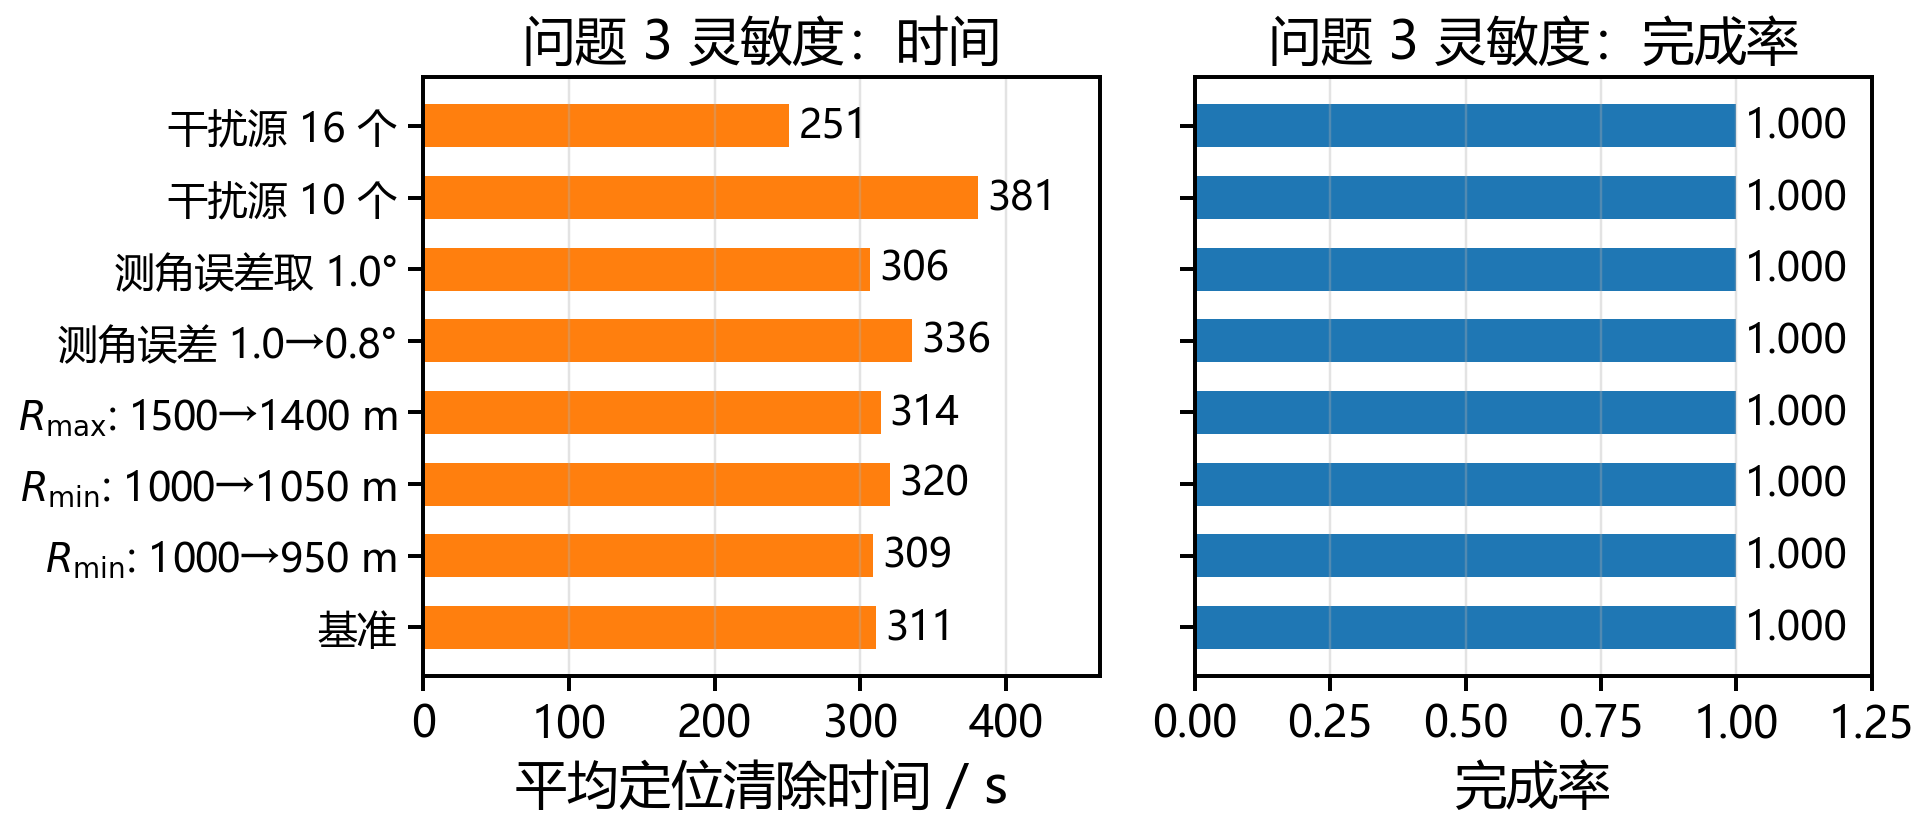
\includegraphics[width=0.78\textwidth]{../figures/fig_q3_sensitivity.png}
\caption{问题三灵敏度：左为完成率，右为平均定位清除时间}
\label{fig:q3sens}
\end{figure}

\begin{figure}[H]
\centering
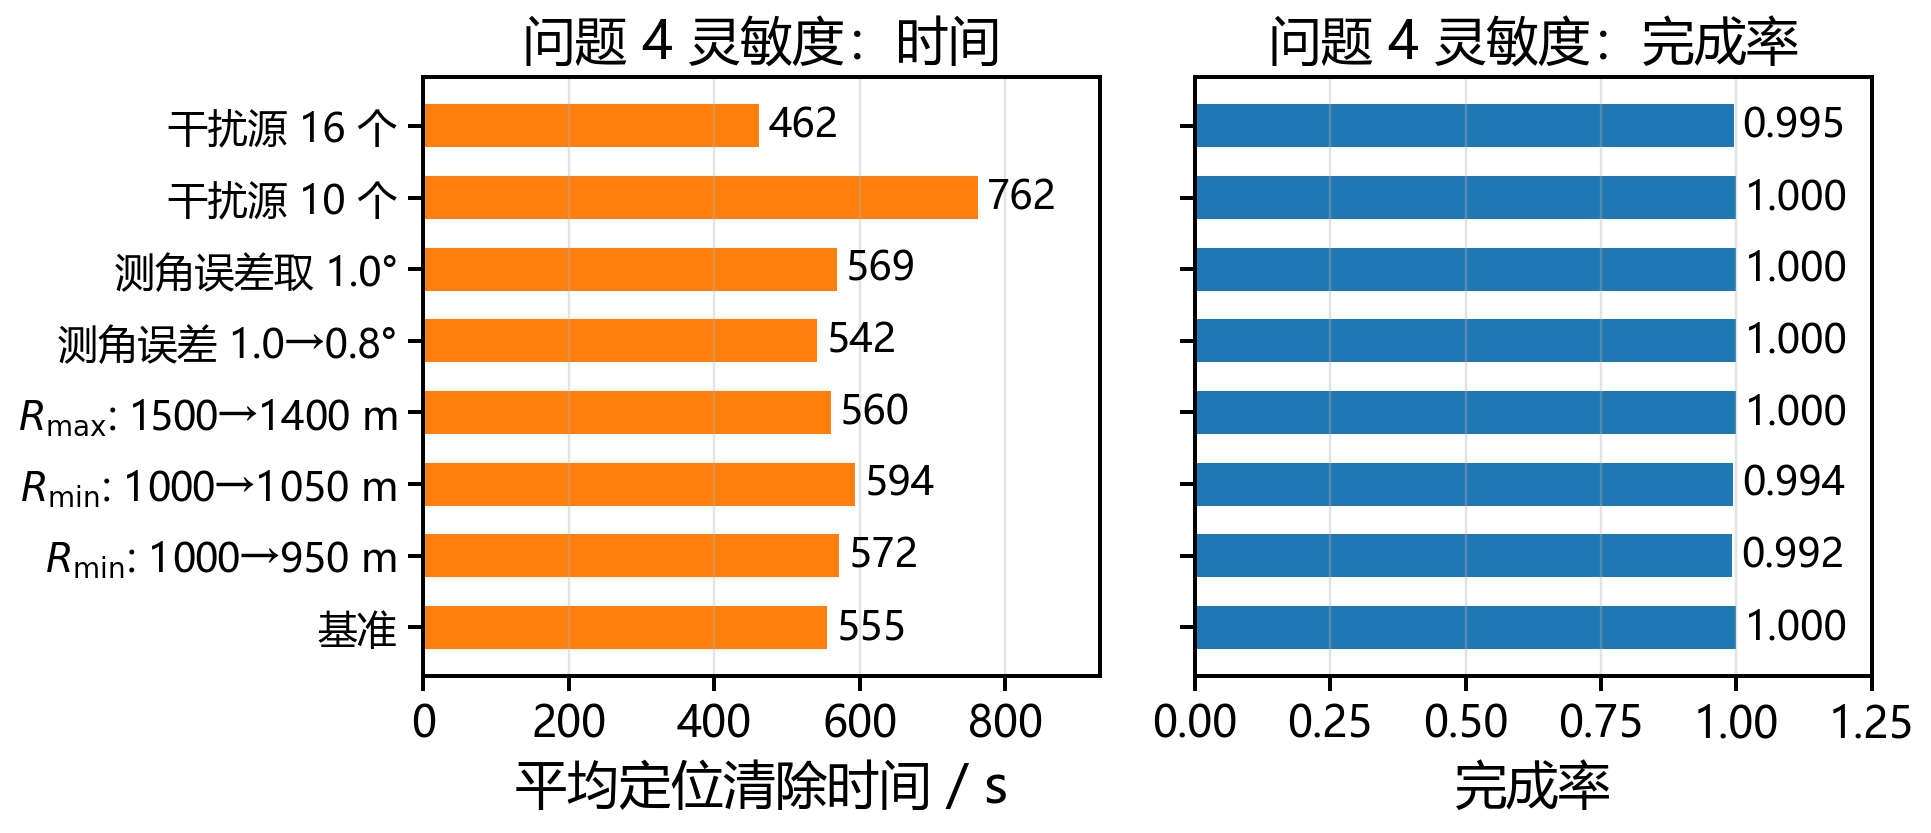
\includegraphics[width=0.78\textwidth]{../figures/fig_q4_sensitivity.png}
\caption{问题四灵敏度：完成率与平均时间对各类扰动的响应均平稳}
\label{fig:q4sens}
\end{figure}

\end{document}
